\documentclass[a4j, 11pt]{jreport}
% START:共通設定&共通パッケージ読み込み(基本変更しない)
\renewcommand{\baselinestretch}{1.4}
\setlength{\oddsidemargin}{-0mm}
\setlength{\textwidth}{16cm}
\setlength{\topmargin}{-1.5cm}
\setlength{\textheight}{24cm}
\setlength{\baselineskip}{2cm}
\special{pdf: minorversion=7}    % 出力するPDFのバージョンを指定
\usepackage{ifthen}              % if文制御用
\usepackage[dvipdfmx]{graphicx}
\usepackage{amsmath}             % 数式用
\usepackage{array}               % 数式での場合分け用
\usepackage{url}                 % URL表示用
\usepackage{here}                % [H]用
\usepackage[dvipdfmx]{hyperref}  % 全体像把握&簡易移動のため
\usepackage{pxjahyper}           % 日本語のしおり(ブックマーク)表示用
\hypersetup{pdfborder = {0 0 0}} % hyperrefリンクの囲みを消す
\pagenumbering{roman}            % ページ番号をアラビア数字に変更
\newcounter{fiscal_year}         % 卒業年度計算用
\setcounter{fiscal_year}{\the\year}
\ifthenelse{\the\month < 4}{
	% 年明けから3月までは年-1にする
	\addtocounter{fiscal_year}{-1}
}{}


% END:共通設定&共通パッケージ読み込み(基本変更しない)


% START:ユーザ設定&ユーザパッケージ読み込み---------
\usepackage{caption}
\captionsetup[table]{justification=centering}
\captionsetup[figure]{justification=centering}
\captionsetup{compatibility=false}

\usepackage{paralist}



% END:ユーザ設定&ユーザパッケージ読み込み-----------


\begin{document}
% START:タイトル
\begin{titlepage}\Large ~
{\normalsize \the\value{fiscal_year} 年度卒業}
\vfill
\begin{center}

% START: 論文の種類-------------------------------
{\Huge 修士論文}
% {\Huge 卒業論文}
% END: 論文の種類---------------------------------
\end{center}
\begin{center}

% START: 日本語タイトル---------------------------
深層学習による銀河形態分類モデルの学習データと異なる空間解像度データへの適用
% END: 日本語タイトル-----------------------------
\end{center}
\begin{center}

% START: 英語タイトル-----------------------------
日本語タイトル暫定版なため,ここ英語タイトルも未完!
% END: 英語タイトル-------------------------------
\end{center}
\vfill
\begin{center}
\begin{tabular}{|c|c|}
\hline

% START: 論文の種類-------------------------------
所属 & \begin{tabular}{c}
  新潟大学大学院自然科学研究科\\電気情報工学専攻・飯田研究室
\end{tabular}\\
% 所属 & 新潟大学工学部情報工学科・林隆史研究室 \\
% END: 論文の種類---------------------------------
\hline

% START: 在籍番号---------------------------------
在籍番号 & F20C026D \\
% END: 在籍番号-----------------------------------
\hline

% START: 論文著者---------------------------------
氏名 & 本間 裕也 \\
% START: 論文著者---------------------------------
\hline
\end{tabular}
\end{center}
\vspace{1cm}
\vfill
\end{titlepage}
\pagebreak
\addtocounter{page}{1}
\thispagestyle{empty}  % このページにページ番号を振らない
% END:タイトル

% START:アブストラクト-----------------------------
\chapter*{概要}
銀河形態分類とは,銀河を見かけの形状により分類する手法を指す.見かけの形状により分類された銀河は,年齢や物質量などの物理的性質にも大きな違いがあることが判明した.このことから,銀河の形状はその成り立ちや進化の過程を反映したものであり,また銀河形態分類は銀河形成の研究において大きな価値を持つ分類手法であると言える.近年の計算機の性能向上により銀河画像データセットの大規模化が進み,専門家による手動形態分類が追いつかなくなったことにより,近年機械学習による自動分類手法が注目されている.機械学習による分類手法は様々存在するが,最新の動向としては畳み込みニューラルネットワーク(CNN)を用いた深層学習による銀河形態分類手法が盛んである.

Tadaki et al.(2020)により,低解像度データで学習を行ったCNN銀河形態分類モデルでは分類できないような天体も,高解像度データを学習データに用いることで分類可能であることが報告された.したがって,分類モデルの精度向上には高解像度銀河データセットとそれに対する正確な形態分類カタログが必要であると言える.しかしながら,一つの天体画像撮像サーベイが完了するのには10年もしくはそれ以上の時間を要し,またそれに対する形態分類カタログが完成するのには更に多くの時間がかかる.

ここで,天体画像撮像サーベイの完了を待たずに高解像度画像データの有用な利用方法を考える.高解像度画像が少量取得できた時点でそれらを用いてモデル学習を行い,低解像度画像で学習したモデルよりも高精度の分類が行えれば,高解像度画像の恩恵を受けることが出来る.しかしながら,学習データとテストデータに用いる画像データの解像度は揃えるのが通例であり,また解像度に差がある場合に正しい分類が行えるかはあまり調べられていない.

本研究では,異なる観測装置データを組み合わせた高精度形態分類モデルの開発を行うため,画像データを学習に用いた深層学習モデルが学習に用いたデータよりも解像度の低い画像データに対し予測を適用できるかについて検証した.また,予測が適用できた場合,学習データとテストデータの解像度差がいくつまでならば高精度な予測を提供できるかについても検証を行った.

\chapter*{Abstract}
English Abstract Here

% END:アブストラクト-------------------------------

% START:目次作成
\newpage
\tableofcontents       % 目次作成
\thispagestyle{empty}  % このページにページ番号を振らない
\pagebreak
\pagenumbering{arabic} % ページ番号をアラビア数字に変更
% END:目次作成


% START:本編--------------------------------------
\chapter{はじめに}
銀河形態分類とは,銀河を見かけの形状によって種類分けする手法を指す.銀河の形態は銀河形成や銀河進化によって形作られている.銀河の形態を調べることで銀河形成や銀河進化の歴史の情報を得られることから,銀河形態分類学は銀河形成や銀河進化の研究に有用な学問と言える.銀河形態分類には分類の際に最も重視する要素別に様々な分類体系が存在する.最も代表的な分類体系と言われるハッブル分類では,見かけの形状を分類の指標とし,銀河を楕円銀河・レンズ状銀河・渦巻銀河の3種に大別した.楕円銀河・レンズ状銀河は渦巻き形状を持たない,古くて大質量の星が多く存在する銀河である.また,渦巻銀河は渦巻形状を特徴とする,若くて星形成も盛んな銀河である.ハッブル分類の他に,渦巻銀河の渦巻腕の細かな差を分類指標に組み込むことでハッブル分類を拡張したドゥ・ボークルール分類や,分類の指標に光の中心集中度や銀河の扁平率などを組み込んだヤーキス分類が存在する.

銀河形態分類は従来専門家による手動分類が行われていた.しかし計算機・観測装置の発達によりSloan Digital Sky Survey(SDSS)\footnote{https://www.sdss.org}やLarge Synoptic Survey Telescope(LSST)\footnote{https://www.lsst.org}のような大規模サーベイ観測プロジェクトが行われるようになると,手動分類では増加する膨大なデータ量への対応が困難になった.この状況を打破するために様々な試みが行われ,その中でもGalaxy Zooプロジェクト\cite{Lintott2008}は市民科学という手法にてSDSSへの膨大なデータ量に対応した.
Galaxy Zooは本来専門知識を持った人間によって行われる銀河形態分類を,多量の一般人ボランティアによる投票形式の分類によって行った.Galaxy Zooは銀河ビッグデータセットに対する銀河形態分類において最も成功した例の一つとなったが,一方で一つ一つの天体に対して必要な人数が多くカタログの完成に時間がかかることが欠点としてあった.そこで,大規模データセットへの銀河形態の効率的な提供として,機械学習が注目された.
Banerji et al.(2010)\cite{Banerji2010}では,初期型銀河・渦巻銀河・点源の3種類の形態分類を機械学習モデルにて行った.Galaxy Zooにて分類済みの天体を教師データとし,そのうち色やプロファイルフィッティングなど12のパラメータについて機械学習モデルを学習させることで,約90\%の精度で分類を行った.

2012年にはKrizhevsky et al.(2012)\cite{Krizhevsky2012}によって1000クラスの画像群を約84\%の精度で分類できるAlexNetと呼ばれる深層学習モデルが開発され,深層学習が機械学習分野で大きく注目されるようになった.それ以前においてもニューラルネットワークという手法は存在したが,複雑な特徴を捉えるために層を深くした際に起こる過学習への対処法が確立されていなかった.しかしながら,AlexNetはDropout\cite{Srivastava2014}やReLu関数\cite{Glorot2011},データ拡張とGPU計算による大規模学習などを導入することで過学習への対処に成功した.
画像分類問題におけるディープラーニングモデルの成功を受けて,Dieleman et al.(2015)\cite{Dieleman2015}は,Convolutional Neural Network(CNN)を用いた深層学習モデルを用いて,Galaxy Zooの派生プロジェクトであるGalaxy Zoo2の形態分類カタログを99\%以上の精度で再現した.深層学習は機械学習のように学習パラメータを指定する必要がない点,大量のデータを用いてモデル学習・テストをエンドツーエンドで行える点などの利点が存在する.Dielemanらによって銀河形態分類問題に対するCNNの有用性が示され,この研究例を機に銀河形態分類問題において深層学習を用いた研究例が多く見受けられるようになった.

深層学習を用いた銀河形態分類の研究例として2つの論文を紹介する.
Cheng et al.(2019)\cite{Cheng2019}は,銀河形態分類に画像データを使用した場合に最適な機械学習手法を調査した.入力データとしてDark Energy Survey(DES)から取得した天体画像データと,Galaxy Zooから取得した形態ラベルを用いた.ここで,DESとはダークマターの性質を明らかにするための国際的プロジェクトであり,観測装置であるDark Energy Camera(DECam)を用いて何億もの銀河をマッピングする構想をもつ.DECamはSDSSで用いられた観測装置よりも優れた空間分解能をもつ.Cheng et al.(2019)で行われた実験の結果として,10種類の機械学習手法のうちCNNが最も優れた分類精度をもつことが示された.このことから,銀河形態分類問題における機械学習アプローチにて,CNNにて設計された深層学習モデルが優れていることが示された.

また,Tadaki et al.(2020)\cite{Tadaki2020}は,SDSSおよびDESよりも空間解像度の高いHyper Suprime-Cam(HSC)画像データセットを用いて,SDSSを用いた場合には分類が難しいような高赤方偏移帯の天体群への形態分類ラベル付けを行った.この研究の目的は高赤方偏移帯の渦巻銀河の渦の向きを深層学習モデルにて特定することであった.深層学習モデルの学習データには,HSCより取得した天体画像データとTadaki自らが目視で付けた銀河形態ラベルを用いた.ここで,形態ラベルの信頼基準が劣る渦巻銀河画像は学習データから除外した.またTadakiが遠方と定義する赤方偏移$z>0.1$における物理スケール分解能と大きく異なる,分光赤方偏移$z_{spec} < 0.05$の天体は学習データから除外した.これらの条件を学習データに適用し,特徴のはっきりした天体にてモデル学習を行うことで,遠方天体である赤方偏移$z>0.1$以上の天体を含む渦巻銀河群の腕の向きを,約97\%の精度で分類することに成功した.また,学習済みモデルをモデル学習・テストで用いなかった天体群に適用し,低赤方偏移天体からSDSSでは渦巻腕を検出することが難しい$z>0.2$の高赤方偏移天体まで,様々な赤方偏移を持つ渦巻銀河の渦の向きを検出することに成功した.

Tadaki et al.(2020)で示されたように,深層学習モデルに入力する画像の解像度が高ければ,分類精度は向上すると思われる.そのためいずれ登場するであろう,従来より高分解能を誇る画像データセットは,深層学習を用いて銀河形態分類を行いたい研究者にとって待望されるものである.
しかしながら,撮像を伴った一つの天体サーベイプロジェクトが完了するのには膨大な時間がかかる.従って,今後登場するであろう高解像度画像データセットを用いて銀河形態分類モデルを学習するような研究を行いたい場合,サーベイプロジェクトの完了を待たなければならず,研究の開始までに同じく膨大な時間がかかってしまう.ここで,プロジェクトの完了を待たずとも高解像度画像データが少量取得できた時点でそれらを用いてモデル学習を行うことを考える.この少量のデータで学習したモデルにて,従来の低解像度画像データセットに対し高精度の分類が行えれば,高解像度画像データセットの完成を待たずして,高解像度による分類モデルの分類の高精度性の恩恵を受けることが出来る.
そこで本研究では,深層学習を用いて銀河形態分類を行う際,高分解能観測装置から得た画像データにてモデル学習を行い,その学習されたモデルを用いて従来の低解像度画像データセットに対し高精度な形態分類予測を適用することを目的とする.そしてこの目的が達成可能かどうかを調べるため,空間分解能の異なる観測装置データの組み合わせを想定し,深層学習による銀河形態分類モデルが異なる解像度データに使用可能であるかを検証する.

以下,第2章では本研究で使用した深層学習手法について説明する.第3章では本研究で深層学習モデルの学習及び精度検証に用いるデータセットについて説明する.第4章では,異なる解像度データの組み合わせを行う前に,解像度が揃ったデータセットにて分類モデルを学習した結果について述べる.その際,データセット内における不確かラベルの取扱い,およびデータインバランスが分類精度に与える影響を調査した.第5章では,異なる解像度データを用いて分類モデルの学習および精度検証を行った結果について述べる.その後第4,5章の実験結果を受けて,第6章にて本研究のまとめおよび将来課題について述べる.


\newpage
\chapter{ディープラーニング}
ディープラーニングは機械学習手法の一種であり,人間が学習の指標を決めずとも自ら学習データ内の特徴を捉えながら学習を行っていくアルゴリズムである.この「自ら特徴を見つけ出し学ぶ」という特徴から,膨大な量のデータセットであるビッグデータを学習に用いることで,近年様々なタスクを解決に導ける手法として注目されている.ディープラーニングが近年台頭してきた理由として,Tensorflow, Kerasなどディープラーニングモデルが簡単に構築可能になるライブラリが開発された点,またディープラーニングの学習に用いられるビッグデータが蓄積されてきた点,そして計算機が発達し,これら膨大な容量をもつビッグデータを処理できるほどの処理能力を会得した点などが挙げられる.

第2章では,本論文における銀河形態分類モデルの開発に用いられている,ディープラーニングについて説明を行う.
\section{ディープニューラルネットワーク (ディープラーニング)}
ディープラーニングでは,様々な層で構築された\textbf{モデル}と呼ばれるものを扱う.答えの分かっている学習データを用いてモデルを学習させ,テストデータを用いてモデルの性能検証を行い,そしてモデルを用いて答えの分かっていないデータに対し予測を適用する.
この節では,ディープラーニングの中で最も基本的なモデルであるディープニューラルネットワークの歴史,構成および学習について述べる.

\subsection{パーセプトロン}
パーセプトロンとは複数の信号を入力とし,1つの信号を出力するアルゴリズムであり,またニューラルネットワークの起源となったアルゴリズムである.例として2入力のパーセプトロンの概略図を図\ref{fig:pa-septoron}に示す.また,パーセプトロンの動作を数式で表したものを式\ref{eq:pa-septoron}に示す.

\begin{figure}[H]
  \centering
  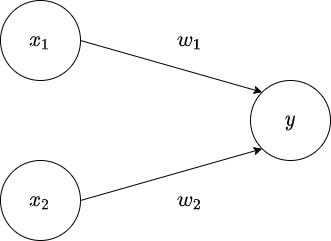
\includegraphics[width=0.50\hsize, keepaspectratio]{images/drawio/pa-seputoron.png}
  \caption{2入力パーセプトロン}
  \label{fig:pa-septoron}
 \end{figure}

\begin{equation}
y= \left \{
\begin{array}{l}
0 (w_1x_1 + w_2x_2 \leq \theta)\\
1 (w_1x_1 + w_2x_2 > \theta)
\end{array}
\right.
\label{eq:pa-septoron}
\end{equation}

2入力パーセプトロンにて$x_1, x_2$は入力信号,$y$は出力信号,$w_1, w_2$は重みである.重みは入力信号に対する''重要度''であり,この値によって入力信号の値が上下する.入力に重みを乗算したものの総和(ここでは$w_1x_1 + w_2x_2$)がしきい値である$\theta$を超えると,パーセプトロンは''発火''し,1を出力する.

パーセプトロンを説明するために,例としてANDゲートをパーセプトロンで表現する.ANDゲートの真理値表を表\ref{tb:and_gate}に示す.このANDゲートをパーセプトロンで表現するためには,適切な重みとしきい値を定めればよい.ANDゲートを表現する$(w_1, w_2, \theta)$の組み合わせとして,例えば$(w_1, w_2, \theta) = (0.3, 0.3, 0.5)$や$(1.0, 1.0, 1.0)$などが考えられる.

$(w_1, w_2, \theta) = (1.0, 1.0, 1.0)$とした場合のANDゲートパーセプトロンを,$x_1$および$x_2$のグラフで表したものを図\ref{fig:pa-septoron_graph}に示す.図\ref{fig:pa-septoron_graph}より,一つのパーセプトロンでは線形の表現しか行えないことがわかる.このため,パーセプトロンは複雑な真理値表のゲートを表現することができない.しかしながら,パーセプトロンの出力を次のパーセプトロンの入力にし,最終的な出力までに複数のパーセプトロンを重ねることで,非線形な表現を行うことが出来る.この方法はニューラルネットワークにおける中間層にあたる.

\begin{table}[H]
  \centering
	\caption{ANDゲートの真理値表}
  \begin{tabular}{cc|c}
    $x_1$ & $x_2$ & $y$ \\ \hline
    0 & 0 & 0 \\ 
    1 & 0 & 0 \\
    0 & 1 & 0 \\
    1 & 1 & 1 \\
  \end{tabular}
  \label{tb:and_gate}
\end{table}

\begin{figure}[H]
 \centering
 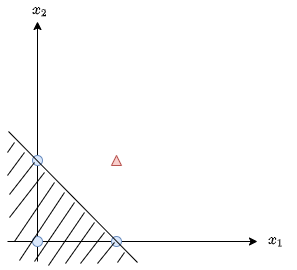
\includegraphics[width=0.5\hsize, keepaspectratio]{images/drawio/pa-seputoron_graph.png}
 \caption{$(w_1, w_2, \theta) = (1.0, 1.0, 1.0)$とした場合のANDゲートパーセプトロン\\(出力が0となる領域を斜線部にて表現)}
 \label{fig:pa-septoron_graph}
\end{figure}

\subsection{ニューラルネットワーク}
ニューラルネットワークとは1986年にパーセプトロンの改良版として考案されたアルゴリズム\ref{}である.パーセプトロンとニューラルネットワークとの違いは主に,単一パーセプトロンでは表現できないような非線形問題を解決できる点,そしてパーセプトロンでは人間の手によって適切に定められていた重みパラメータを,モデルが自ら学習していく点である.

ニューラルネットワークのうち最も単純な構造である,3層ニューラルネットワークの概略図を図\ref{fig:3nn}に示す.円形で表現されているものはノードもしくはニューロンと呼ばれ,それぞれノードは固有の重みを持つ.また,一番左の列を入力層,一番右の列を出力層と呼ぶ.真ん中の列は隠れ層と呼ばれ,単一パーセプトロンではなかった3番目の層が追加されたことにより,ニューラルネットワークは非線形問題のような複雑な問題を解決できるようになった.隠れ層は何層でも重ねることが出来るが,重ねれば重ねるほどに適切な重みを定めることが難しくなる.そこで適切な重みを定めるため考案されたアルゴリズムが,誤差逆伝搬法と呼ばれるものである.誤差逆伝搬法については後ほど詳述する.

\begin{figure}[H]
 \centering
 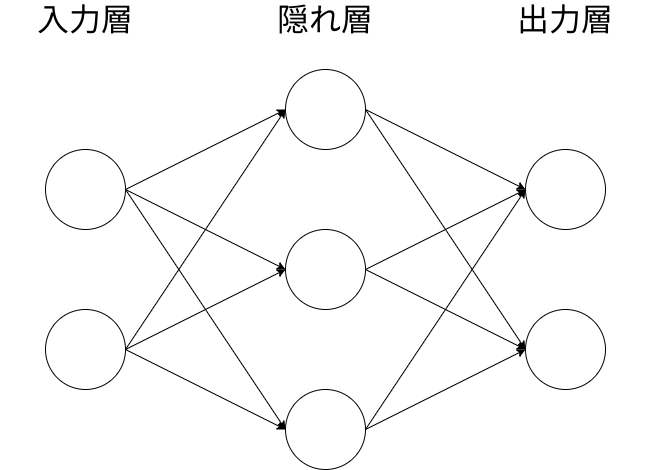
\includegraphics[width=0.7\hsize, keepaspectratio]{images/drawio/3nn.png}
 \caption{3層ニューラルネットワーク}
 \label{fig:3nn}
\end{figure}

\subsection{DNN (Deep Neural Network)}
DNNとはニューラルネットワークにおける隠れ層を多層化,すなわち層を深くしたものであり,現在ディープラーニングと呼ばれているもの全般を指す.ニューラルネットワークにおける隠れ層はせいぜい2,3層であったが,現在使われているDNNでは150ほどの隠れ層をもつこともある.

\subsection{CNN (Convolutional Neural Network)}
CNNとはディープラーニング手法の一つであり,入力データの空間的特徴を捉えて学習を進めていくモデルである.CNNは主に画像認識や音声認識などに用いられる.代表的な学習済モデルとして,AlexNet\ref{}やVGGNet\ref{}などが存在する.DNNのうち最も基本である全結合のニューラルネットワークでは,画像データを入力データにした際,一次元ベクトルに変換されて入力されてしまうため,画像内の形状やエッジなどの空間的特徴を捉えることが不可能であった.しかしCNNでは畳み込み演算とプーリングを用いることで,画像内の重要な空間的特徴を捉えて学習を進めることが可能である.

CNNでは一般的に畳み込み層とプーリング層が交互に続く形で特徴量抽出を行い,出力層の直前に全結合層で特徴量同士を結合させ判断,出力層で最終判断を行い予測を出力する.畳み込み層やプーリング層,それらの具体的な演算については後ほど詳述を行う.

本研究では画像データを学習データに用いるため,CNNを使用した.3層の畳み込み層を持ったモデルである.具体的なモデル形状については実験の章で説明を行う.

\subsection{モデルの過学習}
深層学習において,\textbf{過学習}はしばしば問題として取り上げられる.過学習(オーバーフィッティングとも呼ばれる)とは,学習データに対しモデルが適合しすぎた結果,テストデータに対するスコアが低くなってしまう現象を指す.過学習したモデルは学習データをほぼ完璧に正答することができるが,本来予測を行いたい対象である未知のデータに対しては,正しい予測を行えないことが多い.この未知データに対する予測性能は\textbf{汎化性能}と呼ばれ,機械学習分野にて重視される性能の一つである.

過学習が起こる原因としては,主に学習データの数が足りないこと,データに対してモデル構造が複雑すぎることが挙げられる.これに対し過学習を防ぐ方法は,主に学習データ数を増やすこと,モデルの複雑さを減らすこと,過学習が起きる直前で学習を止めること,そしてモデルの正則化を行うことなどが挙げられる.モデルの正則化とは,モデルが学習できる情報量に制限を掛けるものであり,これによってモデルの学習の量や質を制限し,汎化性能の向上を期待することが出来る.正則化手法で最も主要に扱われているものとして,Dropout\cite{Srivastava2014}が存在する.これは\textbf{層の説明}にて詳述する.




\newpage
\section{層の説明}
DNNにおけるモデルは様々な層で構成されている.それぞれの層には個別の役割があり,これらによってディープラーニングにおける特徴量抽出や予測が実現される.以下では主にCNNにて重要な層について,説明を行う.
\subsection{全結合層}
\subsubsection{全結合層の概要・演算}
全結合層とは全ての入力データを入力・1つの値を出力する層である.全結合層では,入力データのうち「正解の予測により必要なデータはどれか」を示す重みパラメータを学習し,予測の改善を行っていく.

\begin{equation}
 o = h(w_n i_n + b) (n = 1, 2, ... , 全データ数)
 \label{eq:affine}
\end{equation}

ここで,$i_n$は入力,$o$は出力,$w_n$は重み,$b$はバイアス項を指す.全結合層はいかなる種類のDNNにて広く用いられる層である.
\subsubsection{活性化関数}
式\ref{eq:affine}にて,$w_n i_n + b = x$と置き換えると,$o = h(x)$という関係になる.これは入力信号の総和が,$h(x)$という関数によって出力信号に変換されることを意味している.ニューラルネットワークにおいて,層の出力には$h(x)$のような関数が多くの場合存在し,これを\textbf{活性化関数}と呼ぶ.この活性化関数がパーセプトロンとニューラルネットワークとの違いの一つであり,またニューラルネットワークの表現力向上に大きく寄与している.活性化関数の詳しい説明は後の節にて行う.
\subsection{畳み込み層(Conv)}
畳み込み層は,入力データに対しフィルタを適用することで,入力データの特徴抽出を行う層である.畳み込み層において,重みはフィルタの値に相当する.

フィルタサイズ3x3の,畳み込み層における畳み込み演算の概略図を図\ref{fig:conv2d}に示す.畳み込み演算は画像処理におけるフィルター演算に相当し,行列同士の積和演算を行うことで入力データ内の特徴量抽出を果たしている.ここで,フィルタとの積和演算によって生成された行列を特徴マップと言う.

\begin{figure}[htbp]
 \centering
 
\includegraphics[width=0.9\hsize, keepaspectratio]{images/drawio/conv2d.png}
 \caption{畳み込み演算の概略図}
 \label{fig:conv2d}
\end{figure}

このように畳み込み演算を行うことで2次元データ内の空間的特徴抽出が行えるため,畳み込み層は画像分類問題などに適している.

\subsection{プーリング層}
プーリング層とはCNNにて畳み込み層と共に用いられる層であり,特徴の次元削減を行う層である.プーリング層は畳み込み層によって作成された特徴マップに対し,最大値を残す\textbf{最大プーリング},平均値を得る\textbf{平均プーリング}によって次元削減を行う.2x2の最大プーリングの概略図を図\ref{fig:maxpooling}に示す.

プーリング層の重要な役割として,
\begin{inparaenum}[(1)]
 \item 特徴マップの抽象化
 \item 特徴マップ内の平行移動に対して頑健(ロバスト)性を付与する
\end{inparaenum}
というものがある.(1)について,プーリング層は画像内の特徴を失わずに次元削減を行うことができる.つまり,画像内の重要な情報を保持したまま画像全体を抽象化出来る.この特性により,モデルにおいて層の浅い部分では画像内の細かな特徴を,層の深い部分では画像内の大まかな特徴を捉えることになり,結果としてプーリング層はモデルの判断基準の多様性向上に繋がっている.(2)について,入力データの小さなズレに対して,プーリング層は同じような結果を返す.すなわち,プーリング層はほぼ同じ形状をもつ(小さなズレのある)画像データにおいて,ズレを吸収する役割を持つ.これにより,モデルに局所パーツの回転・平行移動・スケールへの不変性を付与することが出来る.

\begin{figure}[H]
 \centering
 
\includegraphics[width=0.8\hsize, keepaspectratio]{images/drawio/maxpooling.png}
 \caption{2x2最大プーリングの概略図}
 \label{fig:maxpooling}
\end{figure}

\subsection{Dropout層}
Dropout層とは,モデルの過学習対策であるモデル正則化の一手法であるDropout\cite{Srivastava2014}をモデルにもたらす層である.Dropout層の概略図を図\ref{fig:dropout}に示す.Dropout層が適用されると,ユーザーが指定した確率でモデル内のノードが無視されるようになる.これにより,モデルの汎化性能が向上する.
Dropoutによって汎化性能が上がる理由としては,\textbf{アンサンブル学習}と同様の効果が期待されるからである.アンサンブル学習とは複数のモデルを個別に学習させ,予測出力時にはそれらのモデルの出力の平均を用いるというものであり,これにより学習の性能が上がることが分かっている.Dropoutはノードをランダムに無効化するという処理により,一つのモデルを複数のより小さなモデルに分け,学習毎に毎回違うモデルを学習させる効果をもつ.この処理は,モデルに対しアンサンブル学習に近い挙動を取らせることが可能である.

\begin{figure}[H]
 \centering
 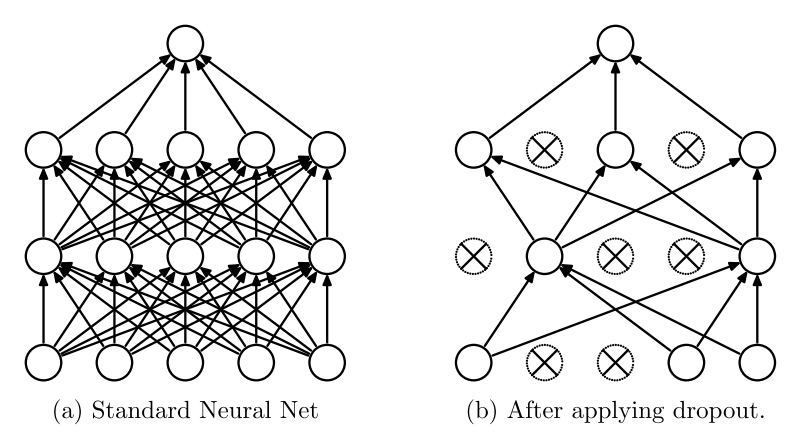
\includegraphics[width=0.8\hsize, keepaspectratio]{images/dropout.png}
 \caption{Dropout層の概略図\\\cite{Srivastava2014}より引用}
 \label{fig:dropout}
\end{figure}


\section{活性化関数}
活性化関数とは,ニューラルネットワークから導入された考え方であり,各層におけるノード内の信号を出力信号に変換する関数である.ニューラルネットワークにおいて,多くの場合活性化関数は非線形である.これは,活性化関数に線形関数を用いると,ニューラルネットワークにおいて層を深くする意味がなくなるからである.線形関数をどんなに深く重ねても,これと同等の処理を持つ関数が非線形関数一つで表せるということが証明されている.これは,非線形関数を用いた場合,ネットワークの層を重ねることでモデルの表現力を大きく向上させられることを意味している.

あらゆる問題に適している活性化関数は今のところ発見されておらず,よって現在までに様々な活性化関数が考案されてきた.以下では代表例として,3つの活性化関数について述べる.
\subsubsection{sigmoid関数}
sigmoid関数は出力信号を-1.0から1.0の範囲に押しとどめる働きをもつ,滑らかな形状をした関数である.ニューラルネットワーク登場時には隠れ層に多く用いられていたが,今では隠れ層にはあまり使われず,2値分類問題の出力層に使われることが多い.

\begin{equation}
 y = \frac{1}{1 + e^{-x}}
 \label{eq:sigmoid}
\end{equation}

\begin{figure}[H]
 \centering
 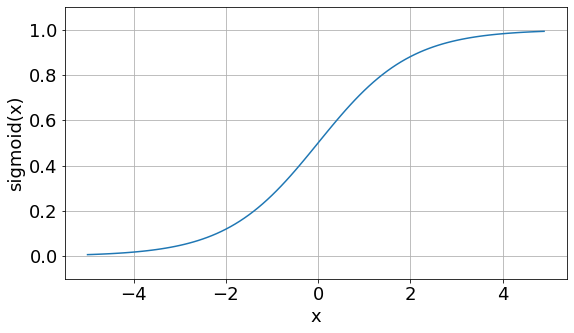
\includegraphics[width=0.7\hsize, keepaspectratio]{images/sigmoid.png}
 \caption{sigmoid関数}
 \label{fig:sigmoid}
\end{figure}

\subsubsection{ReLu関数}
ReLu関数\cite{Glorot2011}は,0以下の信号の場合出力は0とし,それ以上の信号の場合はそのまま出力する関数である.

\begin{equation}
  y= \left \{
  \begin{array}{l}
  x (x > 0)\\
  0 (x \leq 0)
  \end{array}
  \right.
  \label{eq:relu}
  \end{equation}

\begin{figure}[H]
  \centering
  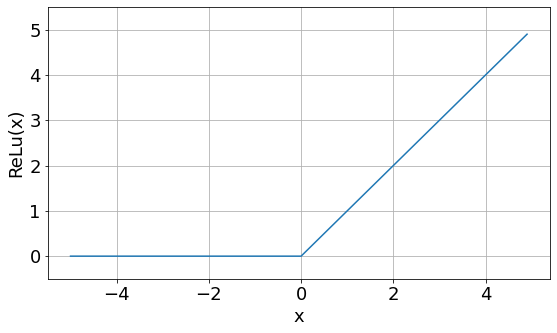
\includegraphics[width=0.7\hsize, keepaspectratio]{images/relu.png}
  \caption{ReLu関数}
  \label{fig:relu}
 \end{figure}

\subsubsection{softmax関数}
softmax関数は,多値分類問題の出力層に用いられる活性化関数であり,出力として「それぞれのラベルである確率」を導出する.$n$クラス問題において,最終層における$i$番目のユニットの出力を$x_{i}$とすると,softmax関数は式\ref{eq:softmax}のように定義される.

\begin{equation}
 y_{i} = \frac{e^{x_{i}}}{\sum_{k=0}^{n}e^{x_{k}}}
 \label{eq:softmax}
\end{equation}

\section{損失関数と重み更新}
\subsection{損失関数}
深層学習の学習で用いられる指標を,損失関数と呼ぶ.損失関数には様々な種類が存在し,解く問題の種類によって使い分ける.
一般的な損失関数として,式(\ref{eq:mse})の2乗平均誤差(主に回帰問題に使用) や,式(\ref{eq:cee})のクロスエントロピー誤差(主に分類問題に使用)が挙げられる.式\ref{eq:mse}において,$y_{k}$はニューラルネットワークの出力,$t_{k}$は教師データを表す.また,式\ref{eq:cee}において,$y_{k}$はニューラルネットワークの出力,$t_{k}$は正解ラベルである.

\begin{equation}
	E = \frac{1}{2} \sum_{k} ({y_k} - t_k)^2
	\label{eq:mse}
\end{equation}

\begin{equation}
	E = -\sum_{k}t_{k}\log y_{k}
	\label{eq:cee}
\end{equation}

\subsection{重み更新}
ニューラルネットワークにおいてモデルの学習とは,モデルの予測が正解に近づくように各ノード内の重みやバイアスを更新していく作業のことである.深層学習においてモデルの学習は,教師データとモデルの予測データとの誤差を示す損失関数を最小化する(0にする)ように進める.以下では,深層学習モデルの学習の具体的な方法について説明する.
\subsubsection{誤差逆伝搬法}
誤差逆伝搬法とはニューラルネットワークでよく用いられる,ネットワーク全体に学習を行わせる,すなわちネットワーク全体の重み更新を行わせるための計算手法を指す.モデルによる予測の正答性を向上するためには,損失関数が0になるように各ノードの重みやバイアスを更新していく必要がある.損失関数の数値はモデルの出力層で導出されるため,誤差を指標にネットワーク全体の重み更新を行うには,出力層から入力層へと逆向きに重み更新を行っていく必要がある.これが誤差逆伝搬法の名前の由来である.

ここで,損失関数が0になるようにあるノードの重みを更新する時,損失関数の偏微分を用いる.これは微分はグラフの傾きを表すため,微分が正となる区間では重みを増加させ,負となる区間では重みを減少させればよいからである.誤差逆伝搬法では各ノードにおける損失関数の偏微分量を,合成関数の微分公式である\textbf{連鎖律}を用いて計算することで,膨大な計算量を省略している.
\subsubsection{最適化手法(勾配降下法)}
誤差逆伝搬法がネットワーク全体の重み更新手法のことを指す一方で,最適化手法とは各ノードにてどのように重みを更新するかを決定するアルゴリズムを指す.ここでは,ニューラルネットワークにて最も普遍的に用いられる\textbf{勾配降下法}について説明する.

勾配降下法では,ある一定数の訓練データごとに損失関数の全ての偏微分をまとめた\textbf{勾配}を導出し,また導出した勾配に基づいて重み更新を繰り返していくアルゴリズムである.重み$w$,およびバイアス$b$をもったノードに対する勾配降下法の計算式を式\ref{eq:gradient}に示す.ここで,$\eta$は\textbf{学習率}と呼ばれるハイパパラメータであり,勾配の更新量を決める定数である.学習率は大きすぎると損失関数がいつまでも最小値にたどり着かず,また小さすぎると局所解から抜け出すことができなくなる.解く問題とモデルの構造によって最適な学習率は異なり,よって全てのモデルに適している学習率は存在しない.

\begin{equation}
  \begin{array}{l}
    w_{t+1} = w_t - \eta \frac{\partial E}{\partial w} \\
    b_{t+1} = b_t - \eta \frac{\partial E}{\partial b}
  \end{array}
  \label{eq:gradient}
\end{equation}

\begin{figure}[H]
 \centering
 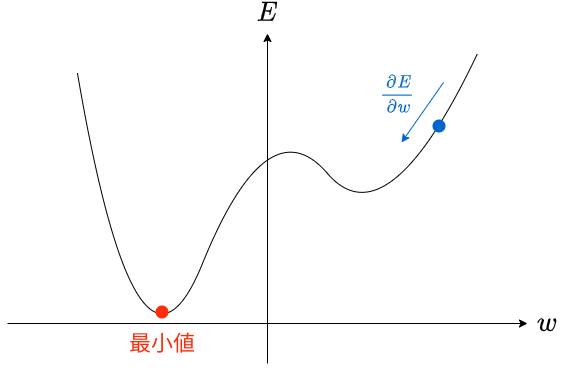
\includegraphics[width=0.7\hsize, keepaspectratio]{images/drawio/gradient.png}
 \caption{勾配降下法の解探索イメージ}
 \label{fig:gradient}
\end{figure}

\newpage
\chapter{使用するデータセット}
\section{Sloan Digital Sky Survey(SDSS)}

SDSS\footnote{https://www.sdss.org}とは,天文学史上最も重要なサーベイ観測プロジェクトの一つとも称される大規模プロジェクトである.このプロジェクトは全天の約1/4の天域において,天体の画像および分光データを取得し,天体カタログを作成することを目的としたものである.SDSSでの撮像・分光データ取得はCCDを搭載した地上望遠鏡によって行われる.SDSSの最初のプロジェクトであるSDSS-I\cite{York2000}は2000年から2008年まで行われ,また対象を銀河系や超新星に絞ったSDSS-II\cite{York2000}が2005年から2008年にSDSS-Iと並行して実施された.その後,太陽系外惑星調査や天の川銀河の構造及び進化などに焦点を当てたSDSS-III\cite{Eisenstein2011}が2008年から2014年に,南天・北天からの銀河系探索などを目的としたSDSS-IV\cite{Blanton2017}が2014年から2020年に行われた.

SDSSで撮影された天体のうち銀河と判断された天体については,後述するGalaxy Zooによって形態分類ラベル付けが行われている.今回の実験では,SDSSとGalaxy Zooから取得した天体の画像データと分類ラベルを銀河形態分類モデル作成に用いる.

GZによって銀河形態ラベル付けが為されたサーベイであるSDSS-IIにおいて,銀河撮像に用いられた測光フィルタはu, g, r, i, zの5つが存在し,これらのフィルタを使用し5つの帯域画像が撮影された.各測光フィルタにて撮影された画像の波長平均値表を示した表を表\ref{fig:dr7_filters}に示す.また,それぞれの測光フィルタのスループット曲線を図\ref{fig:filter_responces}に示す.図\ref{fig:filter_responces}において,横軸は光の波長を示すオングストローム,縦軸はフィルター応答を示している.

\begin{table}[htbp]
  \centering
	\caption{SDSS-IIにおける,銀河撮像に用いられた測光フィルタ一覧\\(https://classic.sdss.org/dr7/instruments/imager/index.html より引用)}
  \begin{tabular}{|c|c|c|c|c|}
		\hline
    u & g & r & i & z \\ \hline
    3551Å & 4686Å & 6165Å & 7481Å & 8931Å \\ \hline
  \end{tabular}
  \label{fig:dr7_filters}
\end{table}


\begin{figure}[H]
 \centering
 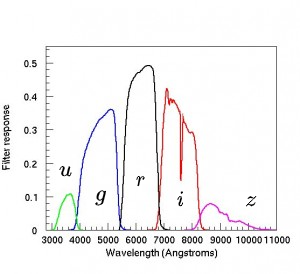
\includegraphics[width=11cm]{images/drawio/filter_responces.png}
 \caption{SDSS-IIにおける測光フィルタのスループット曲線\\(https://www.sdss.org/instruments/camera/ より引用)}
 \label{fig:filter_responces}
\end{figure}



\section{Galaxy Zoo (GZ)}
GZ\cite{Lintott2008}とは,人間の目による分類を行い銀河形態カタログを作成したプロジェクトである.従来の銀河形態分類は専門知識を持った天文学者のチームによって行われてきたが,SDSSのような何十万もの銀河が格納されたデータセットが登場するに従い,天文学者だけでは銀河データの増加に追いつけなくなってきた.このような状況を打破する方法として,インターネットを通じて専門知識を持たない有志の一般人に投票形式で形態分類を行わせる方法が提案された.これがGZである.

GZの最初の調査であるGalaxy Zoo 1\cite{Lintott2010}は2007年7月から2009年2月に行われた.Galaxy Zoo 1による調査の対象となった天体は,SDSSの測光パイプラインによって銀河の判定された天体,またはSDSSの分光観測に含まれていた天体のうち,スペクトルの性質から銀河に分類された天体であり,計893,212個の銀河がカタログに登録された.
Galaxy Zoo 1より詳細な形態分類を行うため,後継プロジェクトであるGalaxy Zoo 2\cite{Willett2013}が2009年2月から2010年4月まで行われた.詳細な形態分類を行うためには天体画像内の形態的特徴がよりはっきりしたものである必要があるため,Galaxy Zoo 2で取り扱った天体はSDSSの最も明るい約25\%の天体である,304,122天体であった.

Galaxy Zoo 1では,ウェブサイト(www.galaxyzoo.org)を通じて有志の一般人の形態分類を投票形式で集計した.サイトを訪れた有志の一般人はウェブサイトにて提示されたカラー銀河画像を見て,時計回り腕をもつ渦巻銀河・半時計回り腕を持つ渦巻銀河・エッジオン(地球から見ると幾何学的に薄い螺旋構造を真横に見る銀河)・楕円銀河・星もしくは分からない天体・マージャー(2つの銀河が衝突し合体している,合体銀河)の6つのうちいずれかに投票を行う.形態分類カタログは,対象となった銀河に対し,各形態分類の投票率を付与され作成される.本研究では,Galaxy Zoo 1で作成された銀河形態カタログから,渦巻銀河・楕円銀河・銀河形態の不確かな天体(以下,不確かな天体と呼称)の3つの分類ラベルを用いて,モデル学習を行う.

% Galaxy Zoo 1の後継プロジェクトであるGalaxy Zoo 2\cite{Willett2013}では,Galaxy Zoo 1より詳細な形態分類を行うため,決定木方式で形態分類を集計した.決定木は11個の分類タスクで構成されており,合計37個の分類が導かれる.各分類タスクは質問とそれに対する回答のセットで成り立っている.(このあと,GZ2の論文から引用した決定木のやつを貼る・それについて説明する)



\section{実験に使用するデータセットの作成方法}
\subsection{天体画像データ}
本研究分類モデル学習に用いる天体画像データとして,SDSS-IIにおけるデータリリースの中から,Data Release 7 (以下,DR7)\cite{Abazajian2009}より画像データを取得した.SDSS-IIにおけるデータリリースにはDR6とDR7が存在する.DR7はDR6の改良版であり,DR6では取得されていなかった天域の追加等が行われている.DR7では3億5700万天体の測光調査が行われた.
DR7 を選んだ理由としては,GZにおける銀河形態ラベル付けにDR7の銀河画像が用いられたからである.

DR7からの天体画像データ取得は,SDSSのData Archive Server(DAS)\footnote{http://das.sdss.org/www/html/das2.html}を介して行った.データベースから取得できるのは,2048x1489ピクセルのある程度大きな天域の画像である.そのため,モデルの学習に用いるための天体画像を取得した場合,DASから取得した天域画像から対象天体の切り出しを行う必要がある.今回はGZにて形態ラベル付けが為されている銀河の中から15,000天体を対象に,銀河毎に64x64ピクセルのサイズで切り出しを行った.15,000天体を対象とした理由について,本研究では銀河の種類ごとに最大1,000天体をモデル学習およびテストに用いる.その際,楕円銀河を1,000天体以上確保できる数が15,000天体であったからである.

また,DR7から取得できる画像はu, g, r, i ,zの5つの帯域画像が存在する.その中から,今回の実験ではrフィルタから得られた帯域画像を使用した.rバンド画像を使用した理由としては,rフィルタが5つの測光フィルタのうち最も感度がよいからである(図\ref{fig:filter_responces}参照).測光フィルタの感度が高い程,より暗い光を捉えた画像が撮影される.よって,rバンド画像は5つの帯域画像のうち最も銀河の形態的特徴を捉えている可能性がある.

\subsection{形態分類ラベル}
今回分類モデル学習に用いる正解ラベルとして,Galaxy Zoo 1から取得できるTable2の分類フラグを用いた.
Table2はSDSS DR7に掲載されている天体のうち,分光スペクトルデータが観測されていた天体に関して収録されている.DR7における総天体数は3億5700万天体であり,Table2に収録されている天体数は667,944天体である.本研究でモデルの学習およびテストに用いる,銀河画像切り出しを行った15,000天体について,これらはTable2の頭から15,000個分を選びだした天体である.なお,Table2全体の渦巻銀河・楕円銀河・不確かな天体の比率は0.285 : 0.093 : 0.622であり,銀河画像切り出しを行った15,000天体の比率は0.271 : 0.104 : 0.626 であった.
Table2の記載内容の一例を図\ref{fig:table2}に示す.

\begin{quote}
  \begin{itemize}
   \item SDSSにおける天体オブジェクトID (OBJID)
   \item 天体の天球座標 (RA, Dec)
   \item 投票数 (NVOTE)
   \item 各カテゴリの得票率 (P\_EL, P\_CW, P\_ACW, P\_EDGE, P\_DK, P\_MG)
   \item P\_CW, P\_ACW, P\_EDGEの合算にて導出された,楕円銀河の投票率 (P\_CS)
   \item バイアスが除去された投票率 (P\_EL\_DEBIASED, P\_CS\_DEBIASED)
   \item 分類フラグ (SPIRAL, ELLIPTICAL, UNCERTAIN)
  \end{itemize}
\end{quote}

バイアスが除去された投票率について説明を行う.


分類フラグは,渦巻銀河・楕円銀河・不確かな天体の3つが存在する.渦巻銀河および楕円銀河の分類フラグは,分類バイアスの除去を行った得票率が8割を超えた場合に立つ.不確かな天体のフラグは,渦巻銀河および楕円銀河のフラグが立たなかった際に立つ.ここで,渦巻銀河(P\_CS)や楕円銀河(P\_EL)の投票率に関係がない,P\_DKやP\_MGの投票率が最も高い天体については不確かな天体にフラグが成立する.
今回はこの分類フラグを深層学習モデルの学習に用いる.なお,GZにはGalaxy Zoo 1とGalaxy Zoo 2の2つのプロジェクトが存在するが,本研究ではGalaxy Zoo 1の形態分類ラベルを実験に用いるため,今後はGalaxy Zoo 1をGZと呼称する.

\begin{figure}[h]
 \centering
 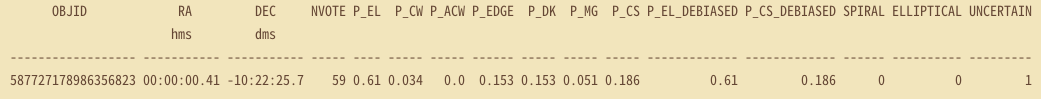
\includegraphics[width=18cm]{images/table2.png}
 \caption{Galaxy Zoo 1にtable2における一例}
 \label{fig:table2}
\end{figure}

\newpage
\chapter{SDSSとGalaxy Zooを用いた分類モデル学習}
この章では本研究の実験に用いられるデータセットであるSDSSとGZにて,学習データとテストデータの解像度が揃っているという条件のもと,どの程度の精度の分類モデルを作成することができるかを確認した.

本研究の将来展望は,高空間分解能観測装置データを用いてモデル学習を行うことで,既存の低空間分解能データセットに対し更なる高精度形態分類を提供するというものである.この将来展望にまつわる実験の最も初段階の前提条件として,まずは学習データとテストデータの解像度が揃っている条件にて学習する銀河形態分類モデルの精度がどのくらいであるかを検証する必要がある.

\section{実験概要}
第4章ではSDSSから取得した銀河画像とGZから取得した分類フラグを学習データとし,渦巻銀河・楕円銀河・不確かな天体のいずれかを予測する分類モデルを学習する.

\subsubsection{用いるデータセット}
実験で用いる天体画像データを作成するため,第3章で説明を行った15,000天体に対し,画像切り出し処理を実行した.その結果,GZにて渦巻銀河とラベル付けがされている天体のうち1天体,および不確かな天体1天体について切り出し処理が正常に行えなかった.切り出し処理の結果として,渦巻銀河4,057天体,楕円銀河は1,561天体,不確かな天体は9,380天体を取得した.
14,998天体の赤方偏移別の個数を示したグラフを図\ref{fig:z_15000}に示す.
ここで赤方偏移とは,地球と対象天体が物理的に遠ざかっている場合や宇宙膨張などにより天体の発する光の波長が伸び,その結果光が赤い方向にずれる現象のこと,あるいはそのずれの大きさを数値化したパラメータのことを指す.
本研究では赤方偏移を後者であるパラメータの意味で用いる.一般的に赤方偏移の値が大きいほど,地球から遠い天体といえる.
渦巻銀河・楕円銀河・不確かな天体の切り出し画像の例を図\ref{fig:sdss_images_spiral}から図\ref{fig:sdss_images_uncertain}に示す.

\begin{figure}[H]
 \centering
 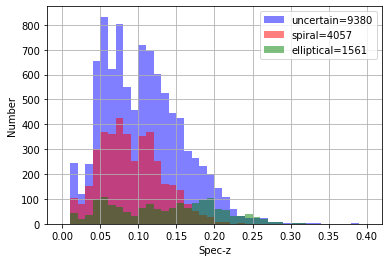
\includegraphics[width=1\hsize]{images/z_15000_0_040_kesson.png}
 \caption{切り出しを行えた14,998天体の分類ラベル別の個数グラフ}
 \label{fig:z_15000}
\end{figure}

\newpage
\begin{figure}[H]
 \centering
 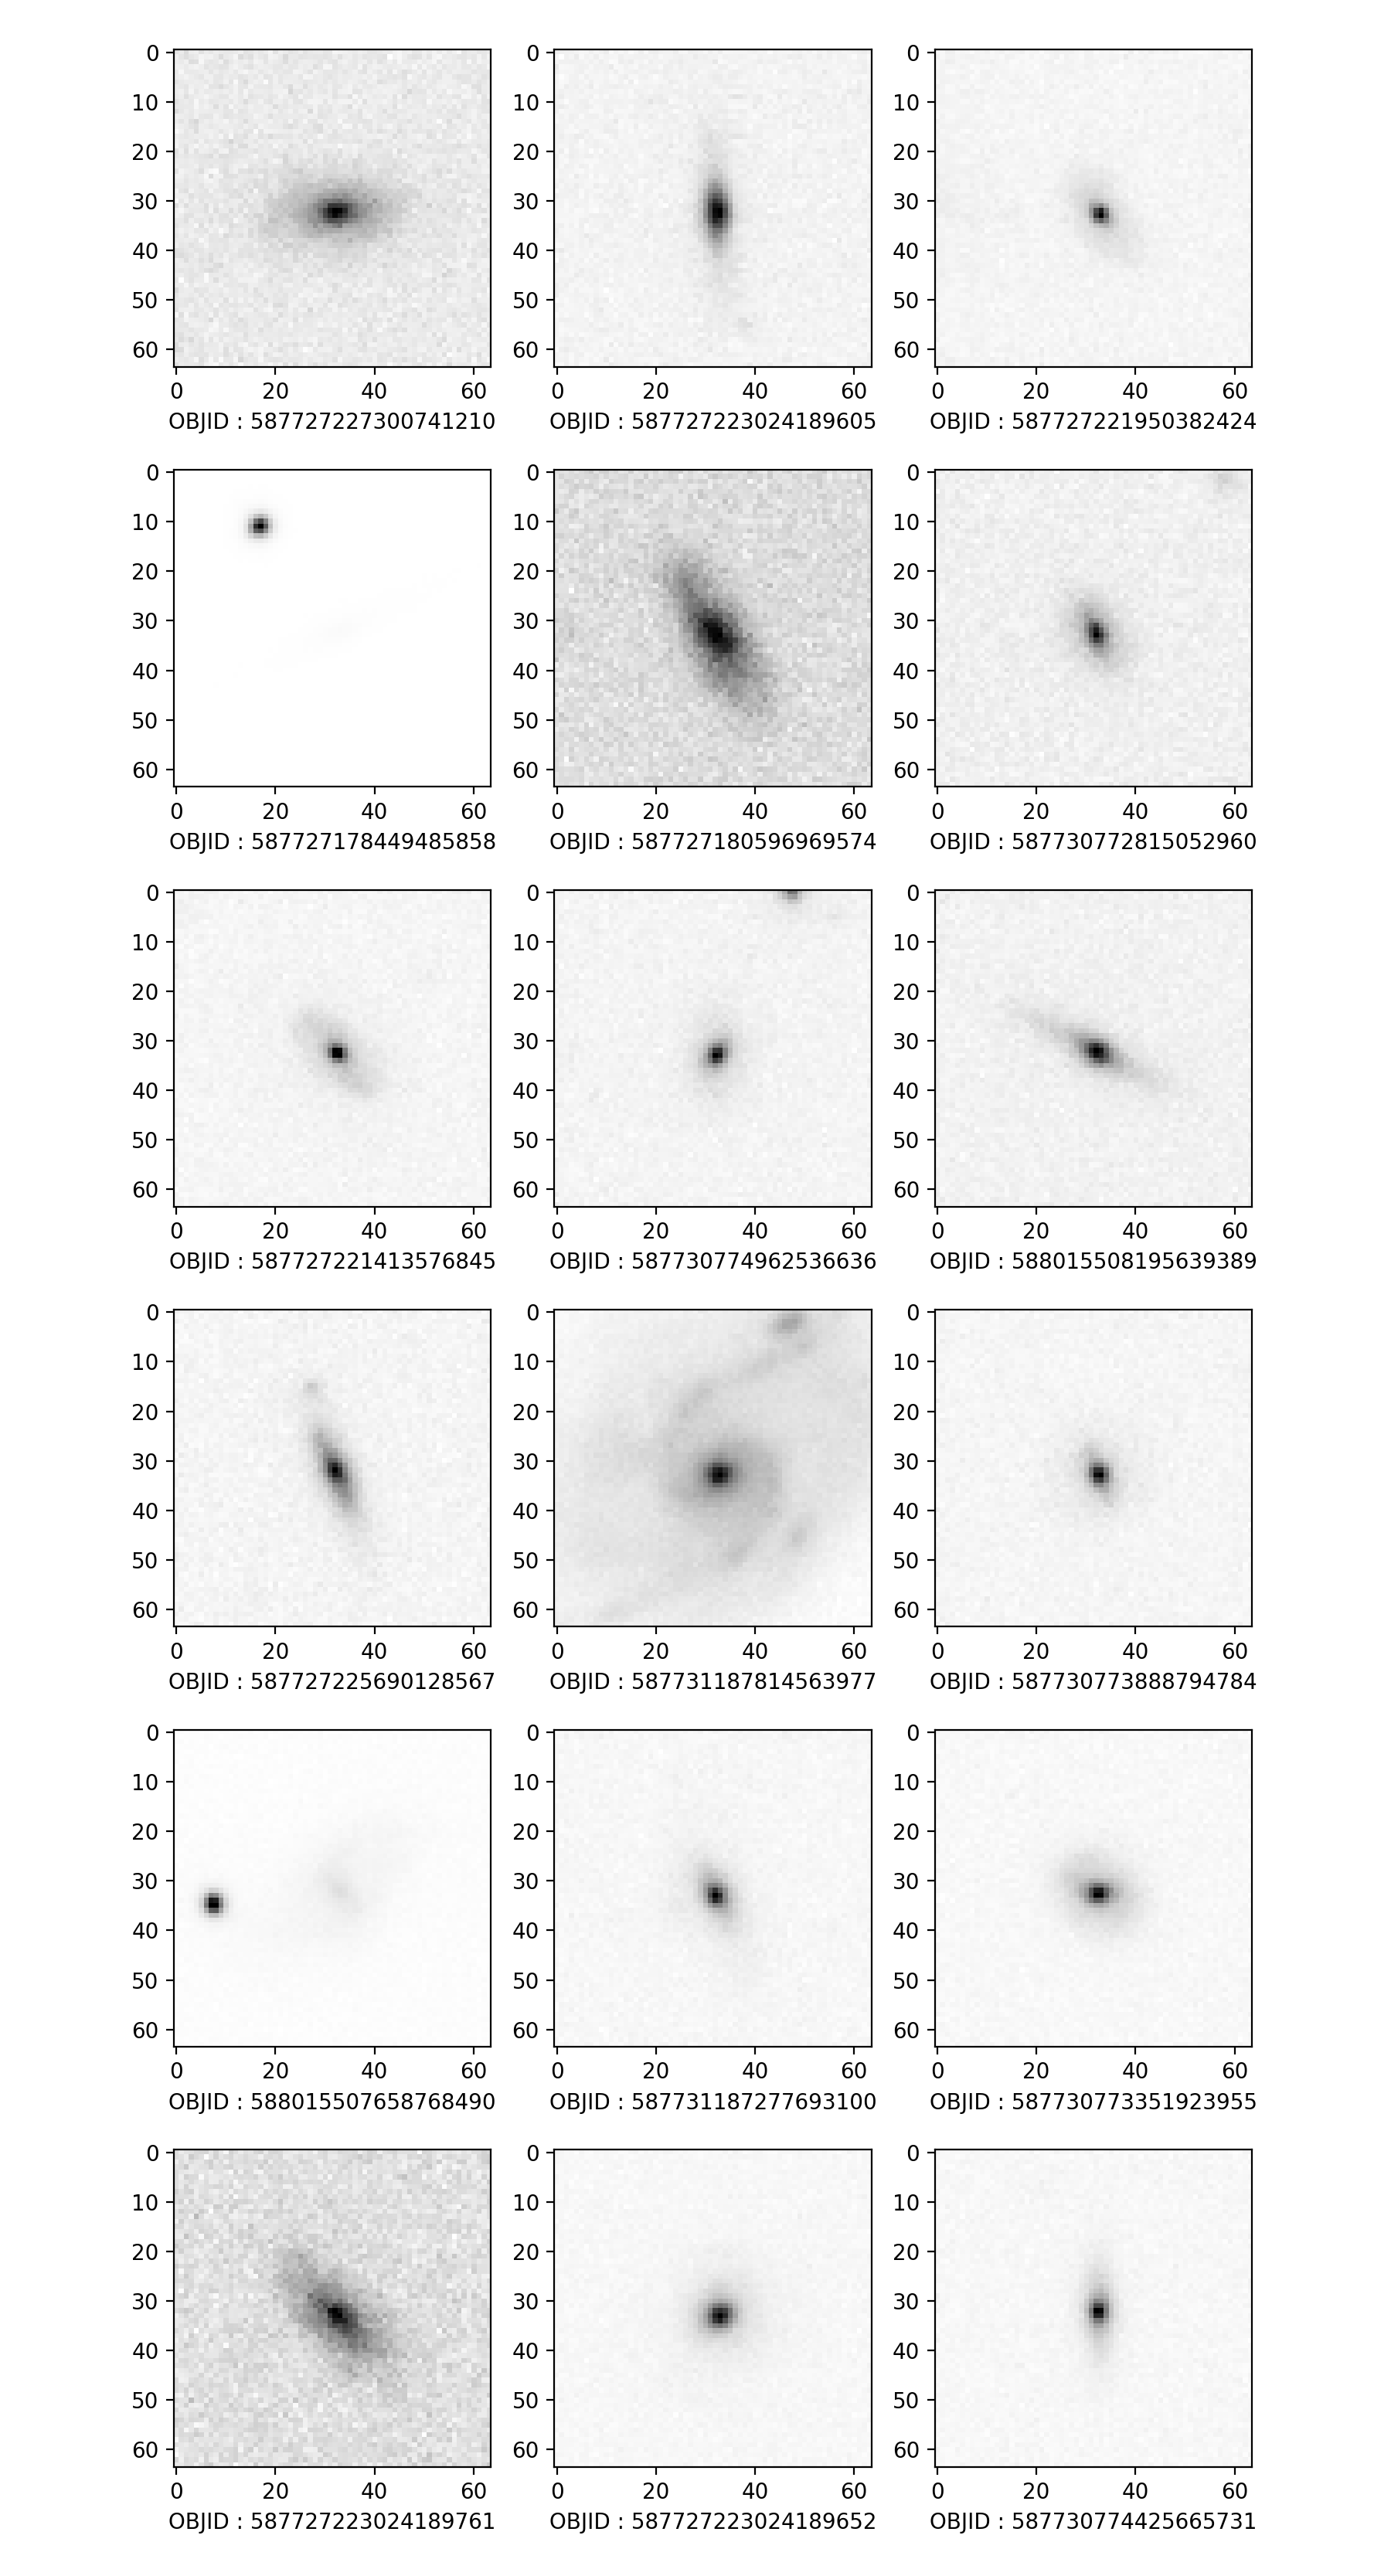
\includegraphics[width=0.5\vsize, keepaspectratio]{images/syuron_4syou_sdss_imgs/spiral_mini.png}
 \caption{渦巻銀河の切り出し画像の例}
 \label{fig:sdss_images_spiral}
\end{figure}

\newpage
\begin{figure}[H]
  \centering
  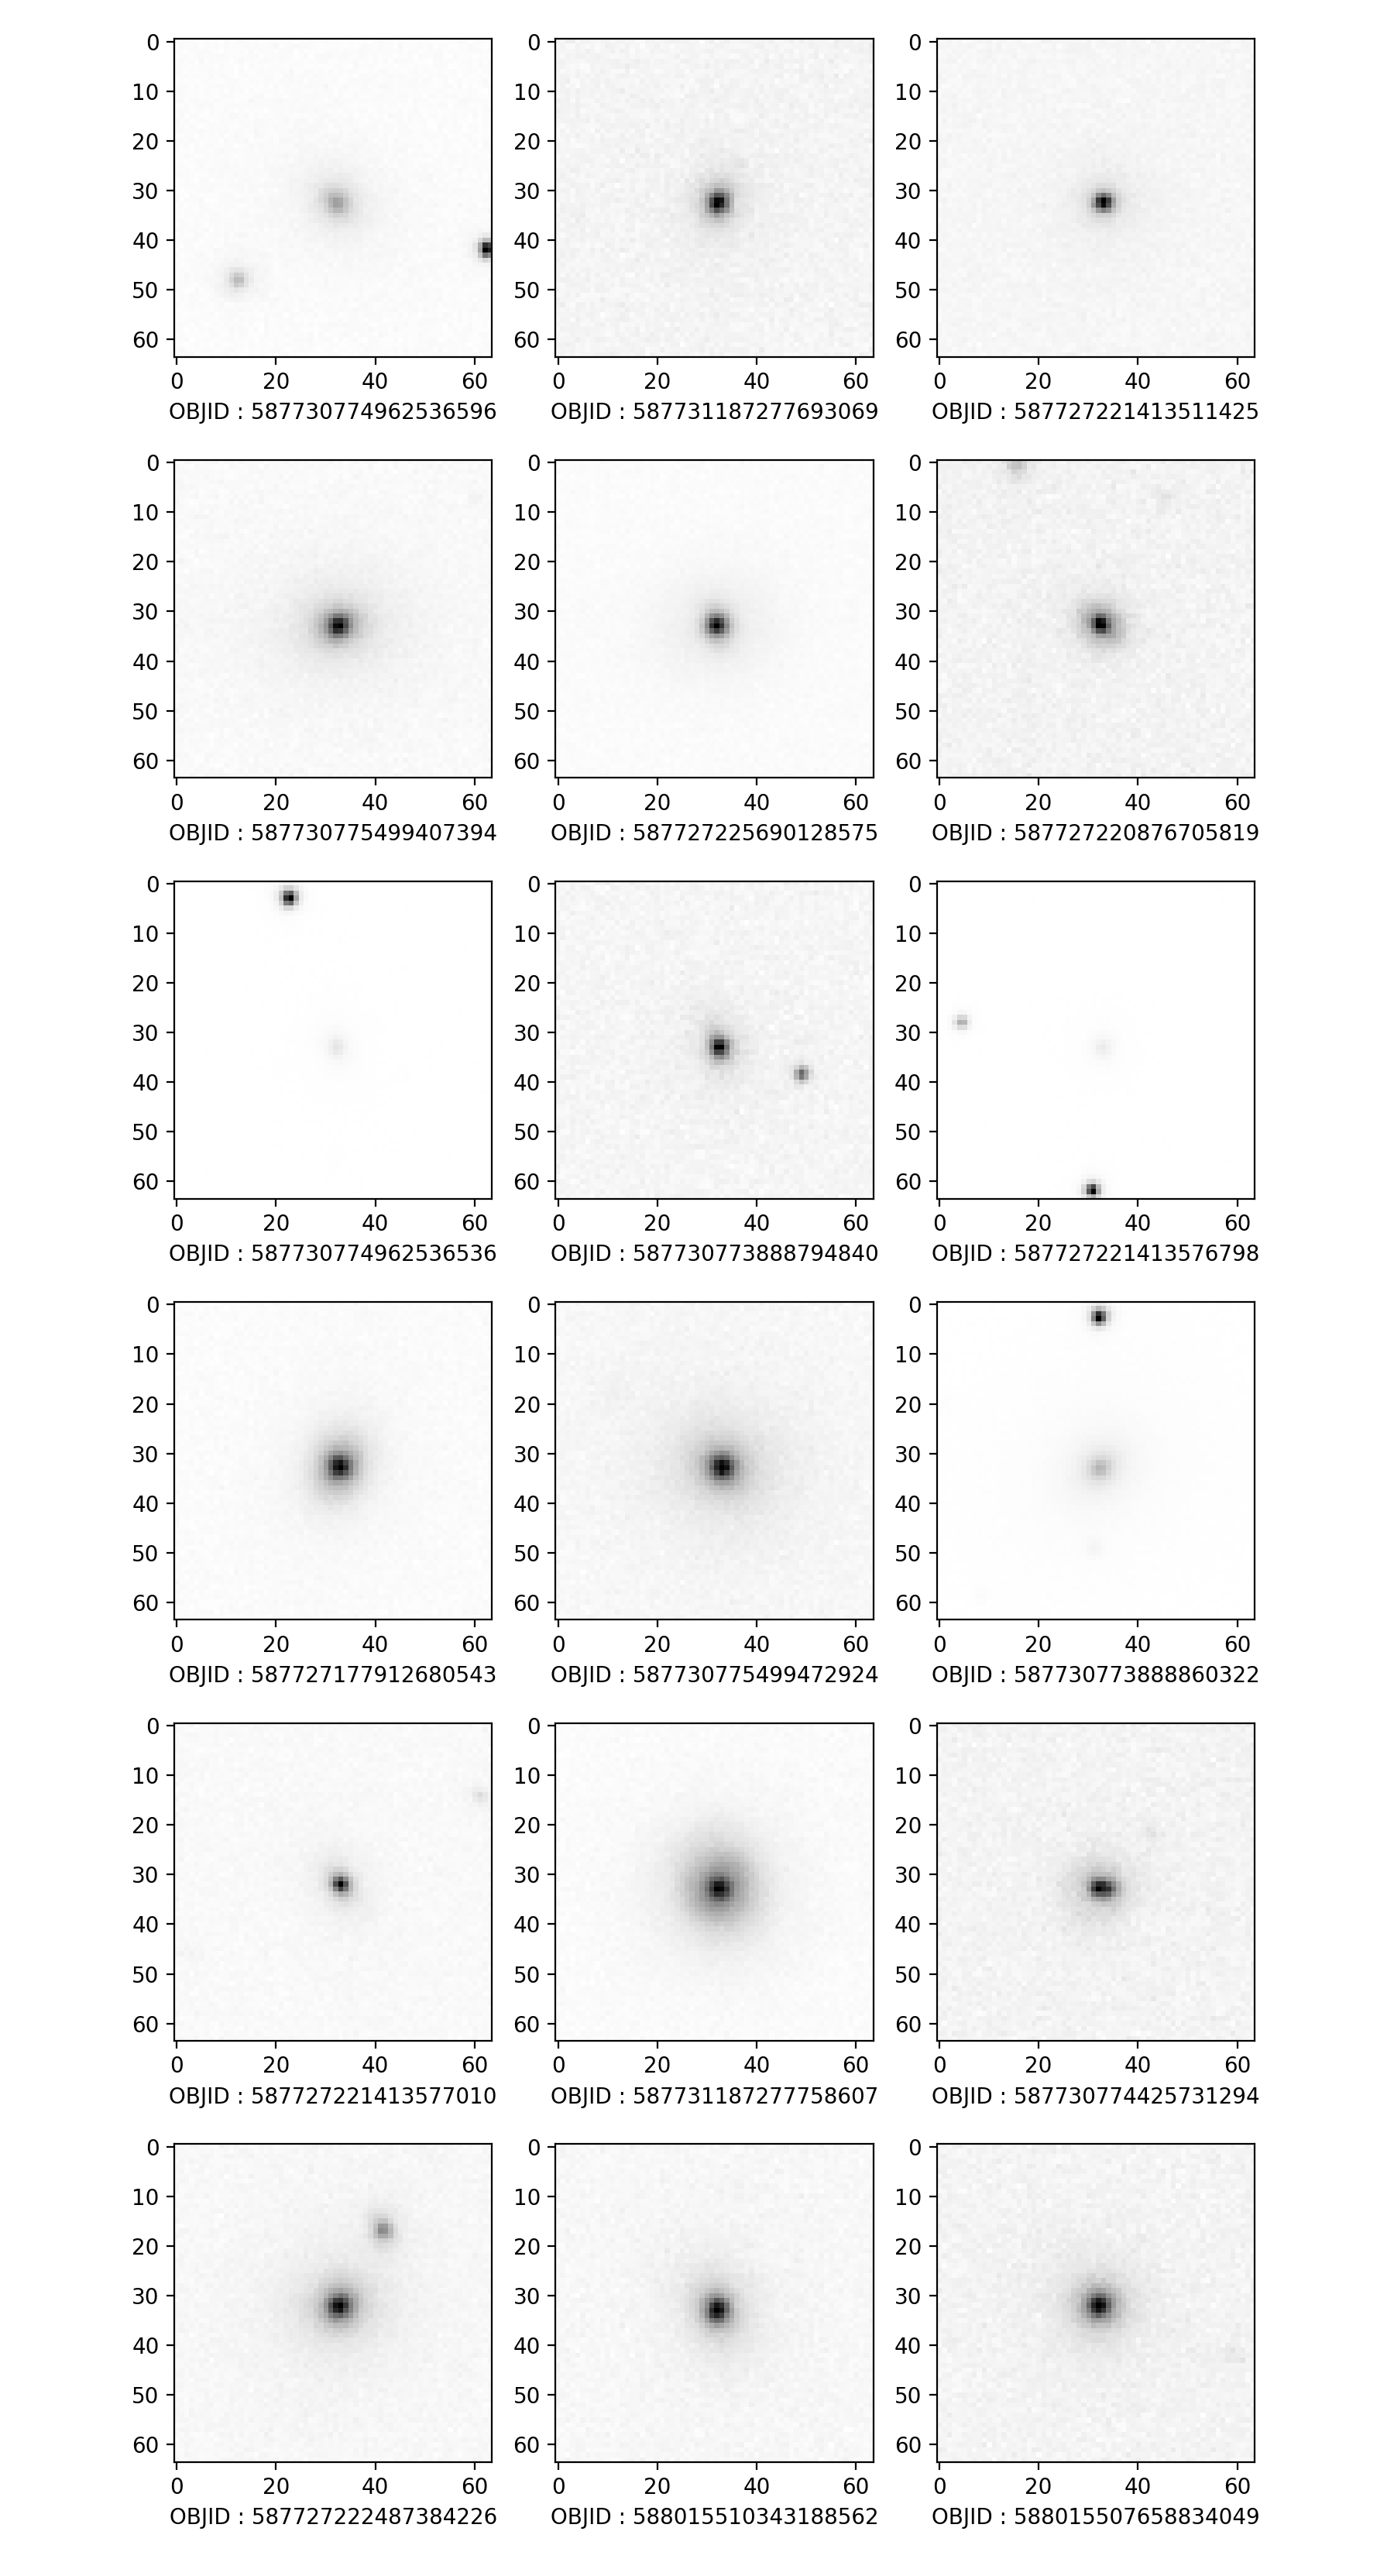
\includegraphics[width=0.5\vsize, keepaspectratio]{images/syuron_4syou_sdss_imgs/elliptical_mini.png}
  \caption{楕円銀河の切り出し画像の例}
  \label{fig:sdss_images_elliptical}
\end{figure}

\newpage
\begin{figure}[H]
  \centering
  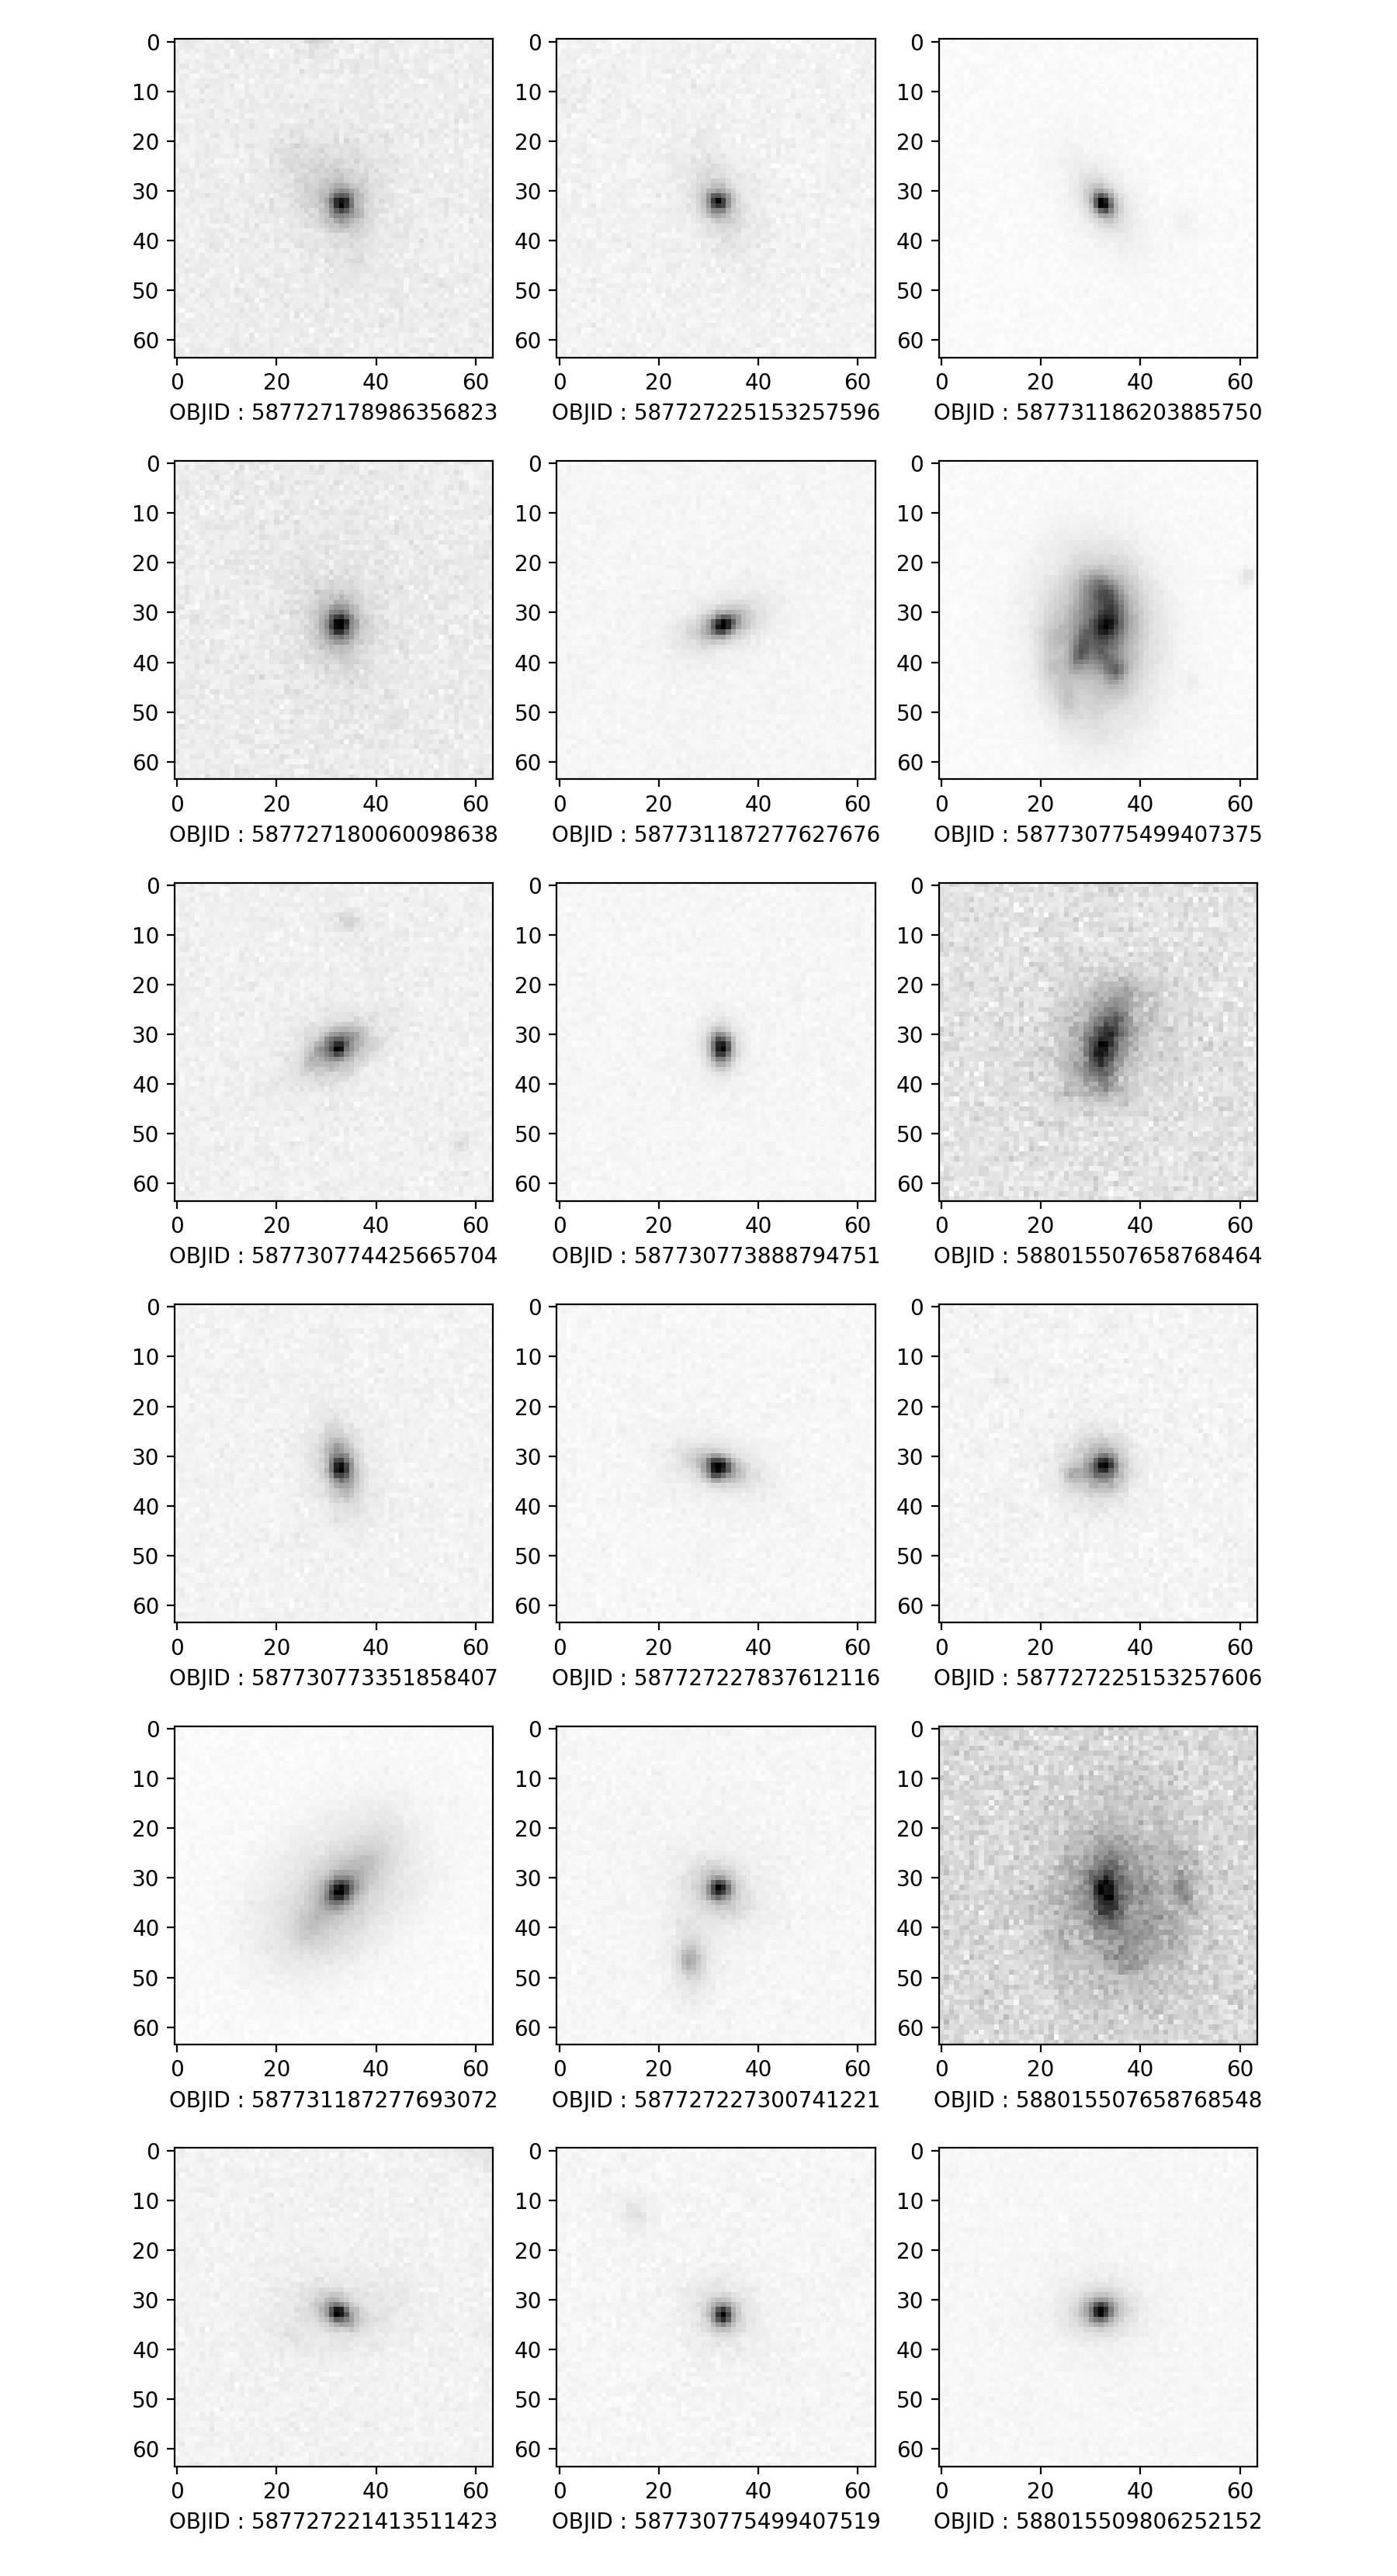
\includegraphics[width=0.5\vsize, keepaspectratio]{images/syuron_4syou_sdss_imgs/uncertain_mini.png}
  \caption{不確かな天体の切り出し画像の例}
  \label{fig:sdss_images_uncertain}
\end{figure}

\subsubsection{モデル構造}
今回用いた深層学習モデルは,Cheng et al.(2019)\cite{Cheng2019}にて用いられていた銀河形態分類モデルを参考にした.Cheng et al.を参考にした理由としては,モデルの学習に用いる形態分類ラベルに本研究と同じGZの形態分類ラベルを採用しており,99\%のaccuracyの分類モデルを作成しているからである.今回用いたモデルの構造を図\ref{fig:model_shape}に示す.このモデルは畳み込み層を合計3つ有しており,それぞれのカーネルサイズは3x3, 3x3, 2x2である.それぞれの畳み込み層の後には,2x2のmax-pooling層が存在する.全畳み込み層の後に全結合層が2層配置されており,それぞれ1024個のノードを有している.損失関数はカテゴリカルクロスエントロピーを使用した.また,活性化関数には確率的勾配降下法を使用し,バッチサイズは8とした.

\begin{figure}[h]
	\centering
	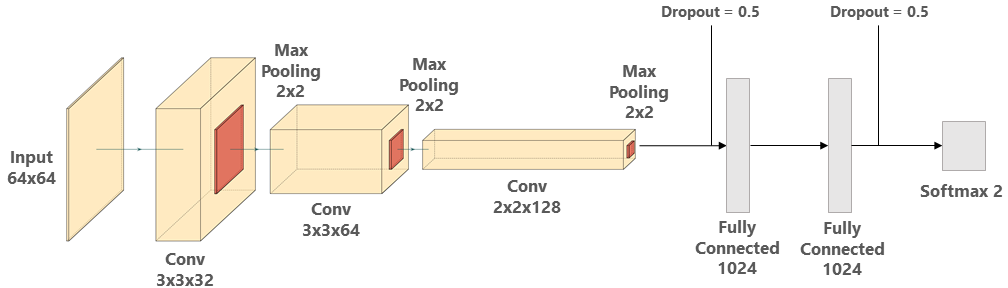
\includegraphics[width=14cm]{images/model_shape.png}
	\caption{用いた分類モデルの構造図}
	\label{fig:model_shape}
\end{figure}
 
\subsubsection{モデルの評価方法}
分類モデルの評価指標として,主にaccuracy (正解率)とtrue positive rate (真陽性率)を用いた.accuracyは全テストデータの中で正しく分類できたデータがどれだけあるかというものであり,モデルの正確性を表す指標である.true positive rateは本来陽性だと分類すべき全データのうち,どれほど正しく分類できたかを表す指標である.accuracyはモデル全体の正確性を表す指標だが,ラベル毎に予測の正確性を判断することはできないため,true positive rateも評価指標として採用している.

以下に2値分類問題を例とした場合の混同行列,accuracy, true positive rateの導出方法を示す.ここで混同行列とは,分類問題においてモデルが予測した値および真の値を行列形式で表したものであり,行成分がモデルによる予測ラベル,列成分がテストデータの真のラベルである.混同行列は分類モデルの性能を可視化・評価するのによく用いられ,モデルの予測値と真の値が交差する対角成分における数が多いほど,モデルが正確な予測を行っているといえる.

\begin{figure}[H]
 \centering
 
\includegraphics[width=12cm]{images/cm.png}
 \caption{2値分類問題における混同行列}
 \label{fig:cm}
\end{figure}

\begin{equation}
 accuracy = \frac{TP + TN}{TP + FP + FN + TN}
 \label{equ:accuracy}
\end{equation}

\begin{equation}
 true positive rate = \frac{TP}{TP + FN}
 \label{}
\end{equation}

\section{不確かラベルが与える分類精度への影響}
GZが与える形態分類フラグのうち「不確かな天体」というフラグが立っている天体は,渦巻銀河・楕円銀河のどちらの得票率も8割を超えなかった天体である.これらの天体は人間の目による形態分類が比較的難しい天体,つまり天体画像から読み取れる形態的特徴があいまいな天体であると考えられる.

この節では特徴があいまいだと考えられる不確かな天体群が,形態分類モデルの分類精度に与える影響を調べる.具体的には,不確かを含めた,渦巻銀河・楕円銀河・不確かな天体の3種類を用いて学習およびテストを行うモデルと,不確かを除いた,不確かを除いた,渦巻銀河・楕円銀河の2種類を用いて学習およびテストを行うモデルをそれぞれ作成し,テストデータに対する予測のaccuracyや混同行列の比較をする.そして不確かな天体の特性や学習に用いた際に分類精度に与える影響を調べる.

\subsection{実験条件(飯田先生へ,実験を行う際の条件なので実験条件が最適だと思うのですが,他にこの節を言い表す言葉はありますでしょうか?)}
モデルの学習およびテストを行う天体数は1,000天体とした.使用する天体は,切り出しを行った14,998天体(図\ref{fig:z_15000}参照)からランダムに取得を行う.取得を行う際,赤方偏移$z$について,$0 < z < 0.2$という条件を設定し,あてはまらない天体は除外を行う.これは,地球との距離が遠すぎる天体を撮影した際,撮影された天体画像は銀河の形態的特徴が上手く捉えられていないことが多く,そのためそれらの画像をモデル学習に用いた場合,分類精度が低下する恐れがあるからである.使用天体を1,000天体取得したあと,学習データとテストデータの比率が7:3となるように切り分けを行った.なお,本論文における学習データとテストデータへの切り分けの際の比率は,特に述べない限り7:3とする.

モデルの評価を行う際,モデルの学習およびテストを30回行い,accuracyの平均値および標準偏差を導出した.なお,30回の学習およびテストの際,学習実行毎に取得される天体は毎回シャッフルされる.
モデルの作成を複数回行う理由としては,深層学習モデルの最終的な分類精度はモデルの重みやバイアスパラメータの初期値依存性と,モデル学習ごとに毎回シャッフルされる使用データへの依存性をもつことから,モデル学習およびテストを複数回行うことでこれら2つの依存性によるモデル分類精度のばらつきを,平均値および標準偏差によって表すためである.


\subsection{実験結果}
不確かを含めた渦巻銀河・楕円銀河・不確かな天体の3値分類モデル,また不確かを除いた渦巻銀河・楕円銀河の2値分類モデルの学習およびテスト結果を図\ref{fig:losses_ex4-1}から図\ref{fig:accs_ex4-2}に示す.図\ref{fig:losses_ex4-1},図\ref{fig:losses_ex4-2}は横軸epoch数・縦軸loss(損失関数)となっている.また,図\ref{fig:accs_ex4-1},図\ref{fig:accs_ex4-2}は横軸epoch数・縦軸accuracy(正解率)となっている.
これらの図において,30回実行の平均値が実線,1標準偏差が透過で示されている.
また,青色のラインが学習データに対するスコア,黄色のラインがテストデータに対するスコアとなっている.lossのグラフについて,学習データに対する損失関数は学習が進むにつれ順当に下がっていくものの,ある一定のepochからテストデータに対する損失関数が上昇していく現象が見受けられる.この現象は\textbf{過学習}と呼ばれている.この現象が起こると,学習データに対し分類モデルが過剰に適合した結果,学習データに対する予測精度に比べテストデータに対する予測精度が低下していく.

また,不確かを含めた渦巻銀河・楕円銀河・不確かな天体の3値分類モデル,および不確かを除いた渦巻銀河・楕円銀河の2値分類モデルの,テストデータに対する予測結果を混同行列で表したものを図\ref{fig:cm_ex4-1}から図\ref{fig:cm_ex4-2}に示す.各セルにはそれぞれ個数の平均値と1標準偏差が示されている.また,個数の平均値によって各セルが色付けされており,色と個数平均値の対応は図右側のカラーバーによって示されている.


\begin{figure}[htbp]
  \begin{minipage}[b]{0.45\hsize}
    \centering
    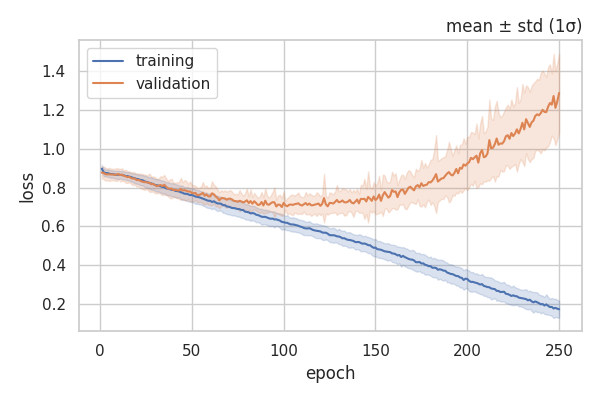
\includegraphics[keepaspectratio, width=7cm]{images/losses_ex4-1.png}
    \caption{3値分類 : loss関数の学習遷移}
		\label{fig:losses_ex4-1}
  \end{minipage}
  \begin{minipage}[b]{0.45\hsize}
    \centering
    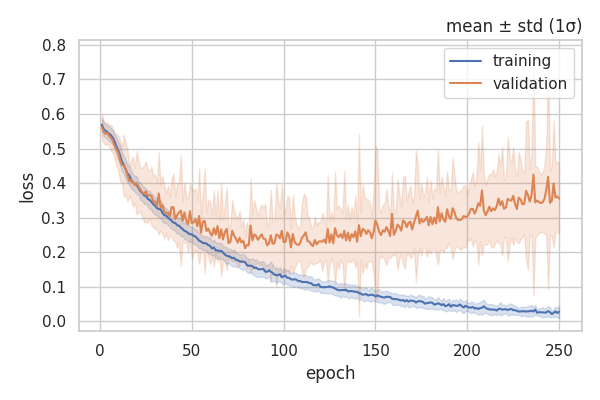
\includegraphics[keepaspectratio, width=7cm]{images/losses_ex4-2.png}
    \caption{2値分類 : loss関数の学習遷移}
		\label{fig:losses_ex4-2}
  \end{minipage}
\end{figure}

\begin{figure}[htbp]
  \begin{minipage}[b]{0.45\hsize}
    \centering
    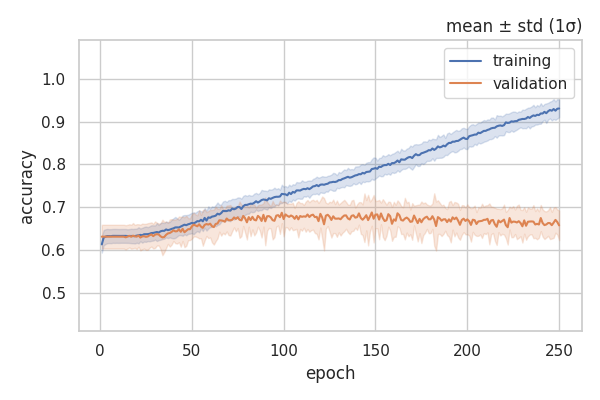
\includegraphics[keepaspectratio, width=7cm]{images/accs_ex4-1.png}
    \caption{3値分類 : accuracyの学習遷移}
		\label{fig:accs_ex4-1}
  \end{minipage}
  \begin{minipage}[b]{0.45\hsize}
    \centering
    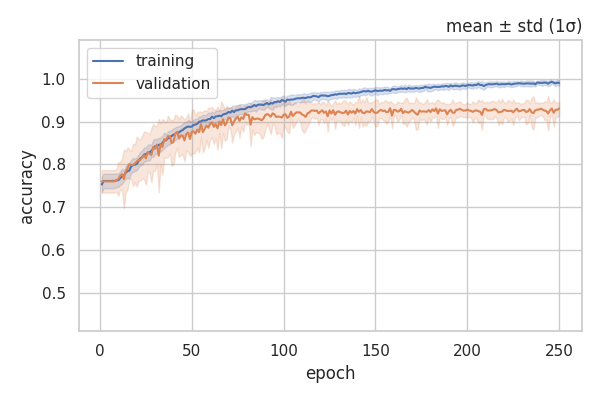
\includegraphics[keepaspectratio, width=7cm]{images/accs_ex4-2.png}
    \caption{2値分類 : accuracyの学習遷移}
		\label{fig:accs_ex4-2}
  \end{minipage}
\end{figure}

\newpage

\begin{figure}[H]
  \begin{minipage}[b]{0.45\hsize}
    \centering
    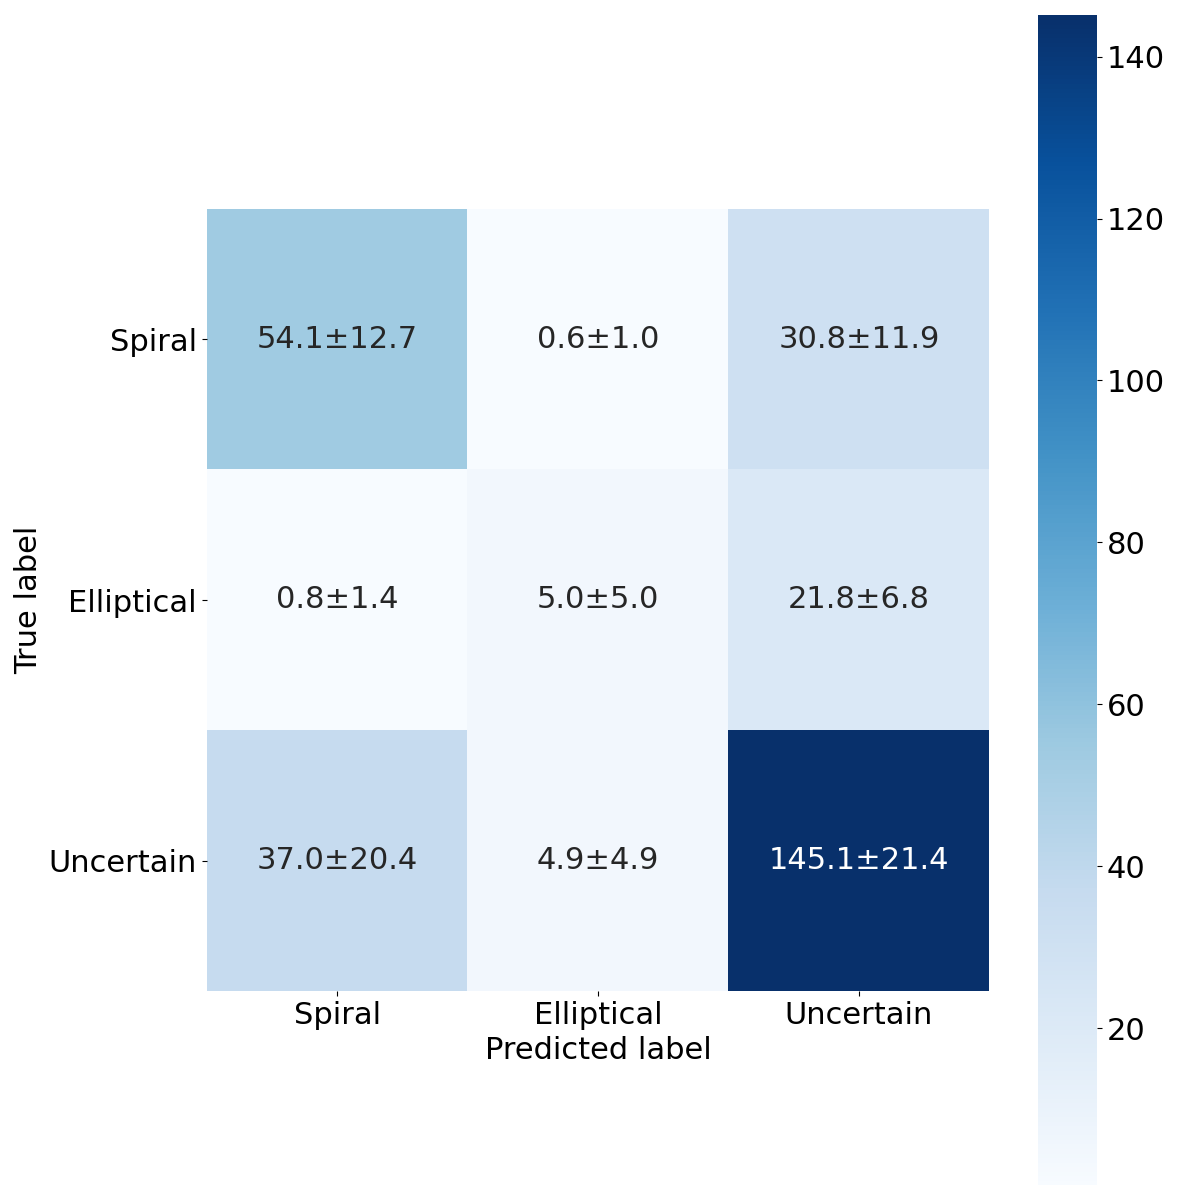
\includegraphics[keepaspectratio, width=7cm]{images/cm_mean_std_ex4-1.png}
    \caption{3値分類 : 混同行列\\(平均$\pm$標準偏差(1$\sigma$))}
		\label{fig:cm_ex4-1}
  \end{minipage}
  \begin{minipage}[b]{0.45\hsize}
    \centering
    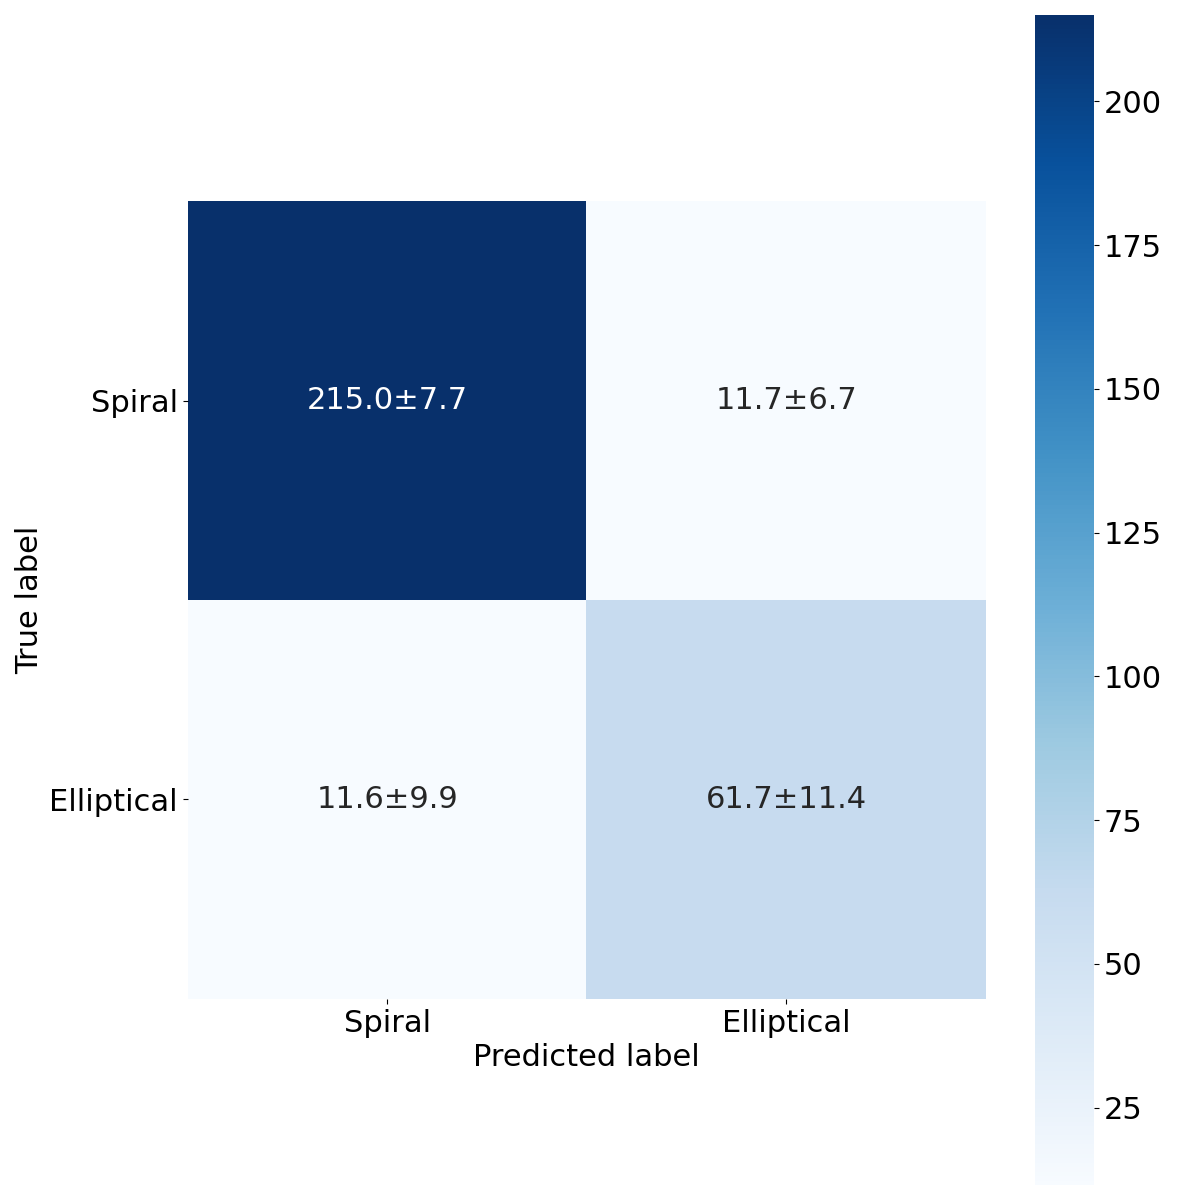
\includegraphics[keepaspectratio, width=7cm]{images/cm_mean_std_ex4-2.png}
    \caption{2値分類 : 混同行列\\(平均$\pm$標準偏差(1$\sigma$))}
		\label{fig:cm_ex4-2}
  \end{minipage}
\end{figure}


% \subsubsection{モデル学習の進行}
% 図\ref{fig:losses_ex4-1}・図\ref{fig:accs_ex4-1}において,テストデータに対するスコアが100epoch付近までloss関数は降下,accuracyは上昇し,それ以降のepochではloss関数が上昇,accuracyが降下していることから,3値分類モデルでは100epochまで学習が良い方向に進んでいるもののそれ以降のepochからはモデルが学習データに対し過学習し,テストデータに対する汎化性能を失っていることが分かる.

% また図\ref{fig:losses_ex4-2}・図\ref{fig:accs_ex4-2}において,テストデータに対するスコアが100epoch付近までloss関数は降下,accuracyは上昇するものの,それ以降のepochではloss関数は上昇するがaccuracyは横ばいになっている.このことから,2値分類モデルにおいては100epoch目以降学習データに対し過適合はしているものの,テストデータに対する汎化性能は失っていないことが読み取れる.

\subsubsection{テストデータに対するaccuracyの評価}
モデルの形態分類性能を評価するため,両モデル間にてテストデータに対するaccuracyの比較を行う.性能評価においては,モデルが学習しきった際の分類性能を用いる.すなわち,accuracyを採るepoch数は,テストデータに対するaccuracyが最大となるepoch数とした.

不確かを含めた渦巻・楕円・不確かの3値分類モデル,および不確かを除いた渦巻・楕円の2値分類モデルにおける,テストデータへの予測精度(accuracy)を表\ref{tb:accs_4.2}に示す.3値分類・2値分類ともに,accuracyを採るepoch数を表内に示している.表\ref{tb:accs_4.2}には,今回の30回実行におけるaccuracyの平均値と標準偏差をそれぞれ1$\sigma$分記載した.

表\ref{tb:accs_4.2}より,標準偏差付き平均値において3値分類モデルと2値分類モデルとの間に有意な差があり,なおかつ2値分類モデルの方がaccuracyが高いことが分かる.

\begin{table}[htbp]
  \centering
	\caption{各モデルのテストデータに対する予測のaccuracy}
  \begin{tabular}{|c|c|}
		\hline
    & mean (1std) \\ \hline
    3値分類(渦巻・楕円・不確か) & $0.688 \pm 0.031$(148th epoch) \\ \hline
    2値分類(渦巻・楕円) & $0.931 \pm 0.017$(158th epoch) \\ \hline
  \end{tabular}
  \label{tb:accs_4.2}
\end{table}

\subsubsection{混同行列の導出方法,および両モデルにおける比較}
次に,混同行列を用いて各モデルのテストデータに対する予測精度の比較を行う.図\ref{fig:cm_ex4-1}より,3値分類モデルにおいて陽性を不確かな天体とした場合のtrue positive rateは$145.1/(37.0+4.9+145.1) = 0.776$だが,渦巻銀河群においては$54.1/(54.1+0.6+30.8) = 0.633$,楕円銀河群においては$5.0/(0.8+5.0+21.8) = 0.181$である.このことから,学習した3値分類モデルは不確かな天体群に比べ渦巻・楕円銀河を正しく分類する性能が劣っており,特に楕円銀河を正しく分類性能することができないことが読み取れる.
図\ref{fig:cm_ex4-2}より,2値分類モデルにおいて陽性を渦巻銀河とした場合のtrue positive rateは$215.0/(215.0+11.7) = 0.948$,楕円銀河とした場合は$61.7/(11.6+61.7) = 0.842$であることが分かる.2つのモデルを比較すると,渦巻銀河と楕円銀河にまつわるtrue positive rateは3値分類モデルより2値分類モデルの方が高いことが分かる.true positive rateはラベル毎の予測の正確性を表す指標であることから,渦巻銀河および楕円銀河を正しく分類する性能は3値分類モデルよりも2値分類モデルの方が優れていることが分かる.

% また,図\ref{fig:cm_ex4-1},図\ref{fig:cm_ex4-2}より,3値分類モデルに用いたテストデータ内には不確かな天体群が約2/3存在し,また2値分類モデルに用いたテストデータ内には渦巻銀河と楕円銀河の比率がおおよそ3:1となっていることがわかる.これは今回用いる天体の母集団である15,000天体(図\ref{fig:z_15000}参照)の特性と一致している.


\newpage
\section{クラスインバランスの影響}
4.2節の図\ref{fig:cm_ex4-1},\ref{fig:cm_ex4-2}より,テストデータにおいて銀河形態ラベルのクラスインバランス(クラスの不均衡)が起きていることがわかった.このインバランスは今回のモデル学習・テストに用いている銀河の母集団(図\ref{fig:z_15000}参照)の性質と一致している.このことから,GZで銀河形態ラベル付けされている天体を深層学習モデルに用いる場合は,クラスインバランスを考慮せねばならず,またこのクラスインバランスがモデルの分類精度に与える影響を調べる必要がある.

この節では,学習データおよびテストデータ内の銀河形態ラベルのクラスインバランスが,形態分類モデルの分類精度に与える影響を調べる.
具体的にはモデルの学習およびテストに渦巻銀河・楕円銀河の比率が異なるインバランスドデータ(不均衡データ)を用いた場合と,渦巻銀河・楕円銀河の比率が等しいバランスドデータ(均衡データ)を用いた場合とで,テストデータに対する予測のaccuracy,true skill statistic(TSS)や混同行列の比較をする.true skill statisticについては,後の実験条件の節にて説明を行う.

\subsection{実験条件}
モデルの学習およびテストを行う天体の選定方法として,インバランスドデータにおいては切り出しを行った14,998天体(図\ref{fig:z_15000}参照)のうち不確かな天体を除いた渦巻銀河・楕円銀河からランダムに1,000天体の取得を行った.またバランスドデータにおいては渦巻銀河と楕円銀河の比率を等しくするために,14,998天体の母集団のうち不確かな天体を除いた渦巻銀河・楕円銀河から,渦巻銀河を500天体,楕円銀河を500天体取得した.また,取得を行う際の赤方偏移$z$の条件は,4.2節と同様の理由で$0 < z < 0.2$とした.
またバランスドデータでは,学習データ・テストデータのどちらも渦巻銀河と楕円銀河の比率が等しくなるように1,000天体からの切り分けを行った.

モデルの評価方法は4.2節と同様の方法で行った.具体的には,モデルの学習およびテストを30回行い,accuracyの平均値および標準偏差を導出した.
なお,30回の学習およびテストの際,学習実行毎に取得される天体は毎回シャッフルされる.
また4.3節の実験においては,モデルの評価指標としてtrue skill statistic(以下,TSSと呼称)の導出も行った.ここでTSSとはaccuracyと同じく正確性を表す指標であるが,テストデータ内のデータインバランス性に対しロバストな性質がある.TSSの式を式\ref{equ:tss}に示す.

\begin{equation}
	TSS = \frac{TP}{TP + FN} - \frac{FP}{TN + FP}
 \label{equ:tss}
\end{equation}

TSSを用いた理由としては,インバランスドデータでのモデル学習・テストにおいて,30回実行における実行毎に取得する天体の渦巻銀河・楕円銀河の比率が毎回異なることから,accuracyだけでは銀河形態ラベルのクラスインバランスを正しく評価できないためである.そこでデータセット内の分類ラベルのインバランス性にロバストな性質をもつTSSも評価指標に加えている.

\subsection{実験結果}
渦巻銀河・楕円銀河の比率が異なるインバランスドデータで学習およびテストを行った2値分類モデル,また渦巻銀河・楕円銀河の比率が等しいバランスドデータで学習およびテストを行った2値分類モデルの学習結果を図\ref{fig:losses_ex4-2-2}から図\ref{fig:cm_ex4-3}に示す.
また,両モデルのテストデータに対する予測結果を混同行列で表したものを図\ref{fig:cm_ex4-2-2}から図\ref{fig:cm_ex4-3}に示す.図\ref{fig:losses_ex4-2-2}から図\ref{fig:cm_ex4-3}の構成は,4.2節における図\ref{fig:losses_ex4-1}から図\ref{fig:cm_ex4-2}と同様であり,最上段は横軸epoch数・縦軸loss(損失関数),中段は横軸epoch数・縦軸accuracy(正解率),最下段はテストデータに対する予測結果を混同行列で表したものである.


\begin{figure}[htbp]
  \begin{minipage}[b]{0.45\hsize}
    \centering
    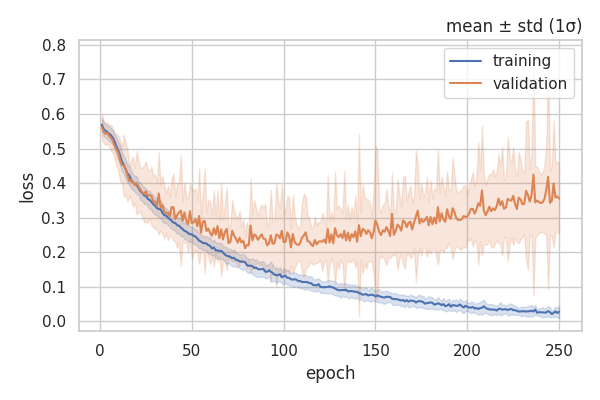
\includegraphics[keepaspectratio, width=7cm]{images/losses_ex4-2.png}
    \caption{インバランスドデータ : loss関数の学習遷移}
		\label{fig:losses_ex4-2-2}
  \end{minipage}
  \begin{minipage}[b]{0.45\hsize}
    \centering
    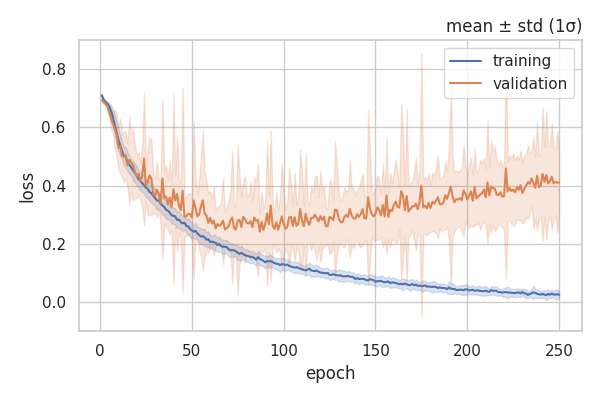
\includegraphics[keepaspectratio, width=7cm]{images/losses_ex4-3.png}
    \caption{バランスドデータ : loss関数の学習遷移}
		\label{fig:losses_ex4-3}
  \end{minipage}
\end{figure}

\begin{figure}[htbp]
  \begin{minipage}[b]{0.45\hsize}
    \centering
    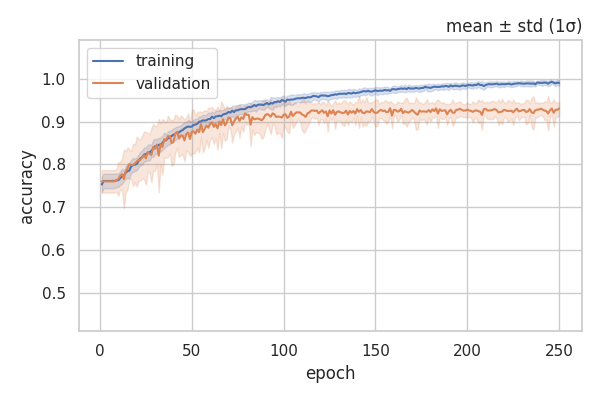
\includegraphics[keepaspectratio, width=7cm]{images/accs_ex4-2.png}
    \caption{インバランスドデータ : accuracyの学習遷移}
		\label{fig:accs_ex4-2-2}
  \end{minipage}
  \begin{minipage}[b]{0.45\hsize}
    \centering
    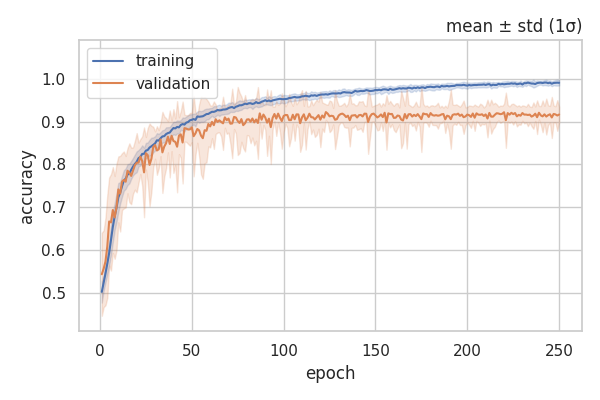
\includegraphics[keepaspectratio, width=7cm]{images/accs_ex4-3.png}
    \caption{バランスドデータ : accuracyの学習遷移}
		\label{fig:accs_ex4-3}
  \end{minipage}
\end{figure}

\newpage

\begin{figure}[H]
  \begin{minipage}[b]{0.45\hsize}
    \centering
    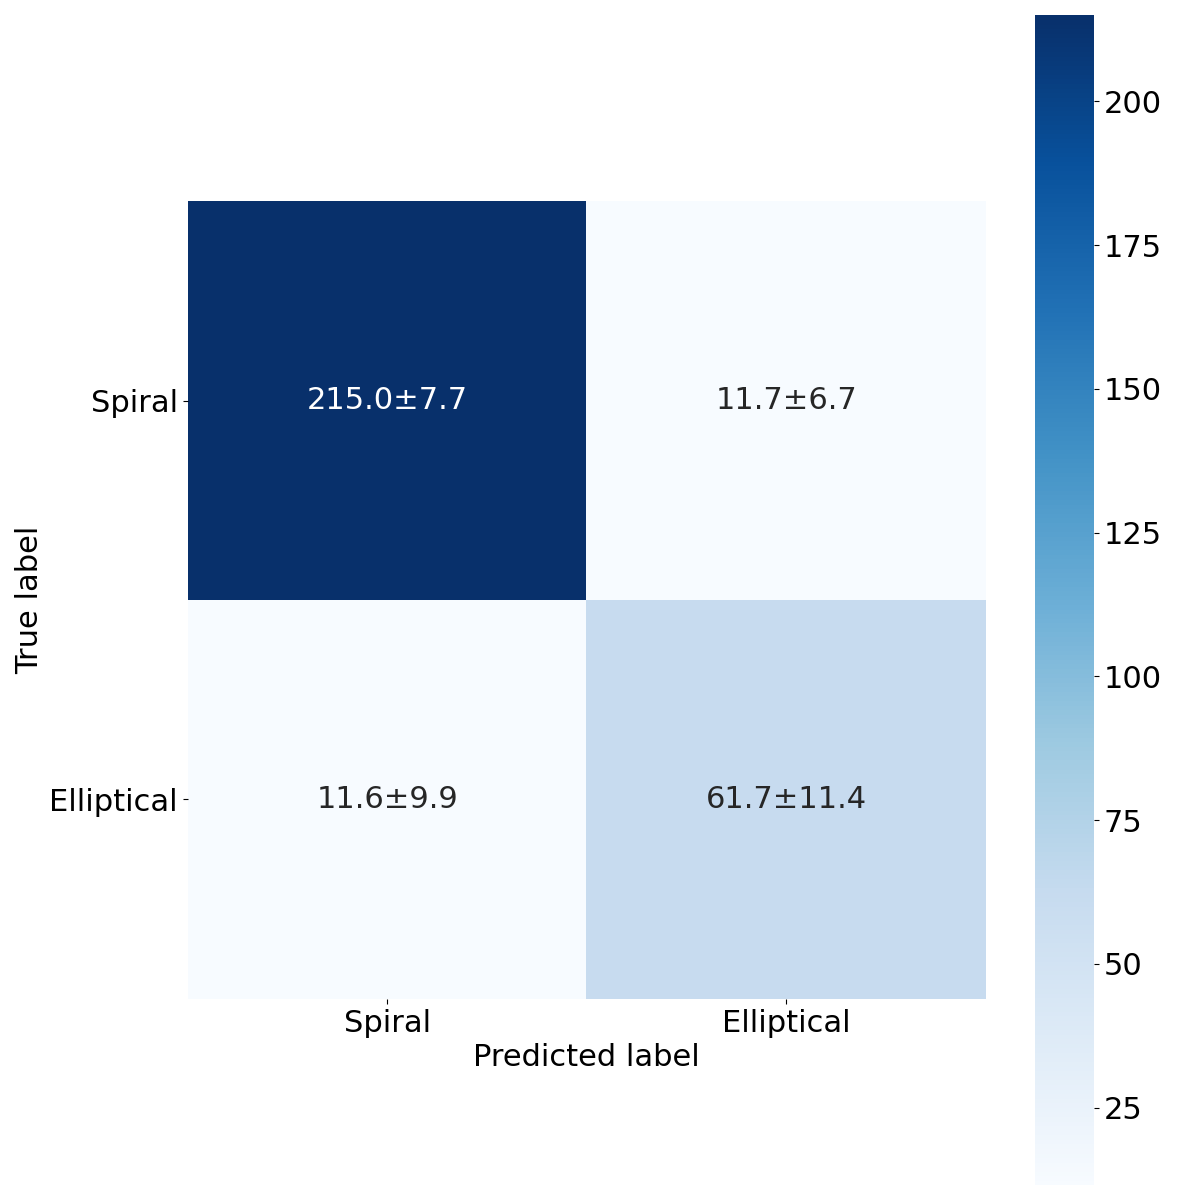
\includegraphics[keepaspectratio, width=7cm]{images/cm_mean_std_ex4-2.png}
    \caption{インバランスドデータ : 混同行列\\(平均$\pm$標準偏差(1$\sigma$))}
		\label{fig:cm_ex4-2-2}
  \end{minipage}
  \begin{minipage}[b]{0.45\hsize}
    \centering
    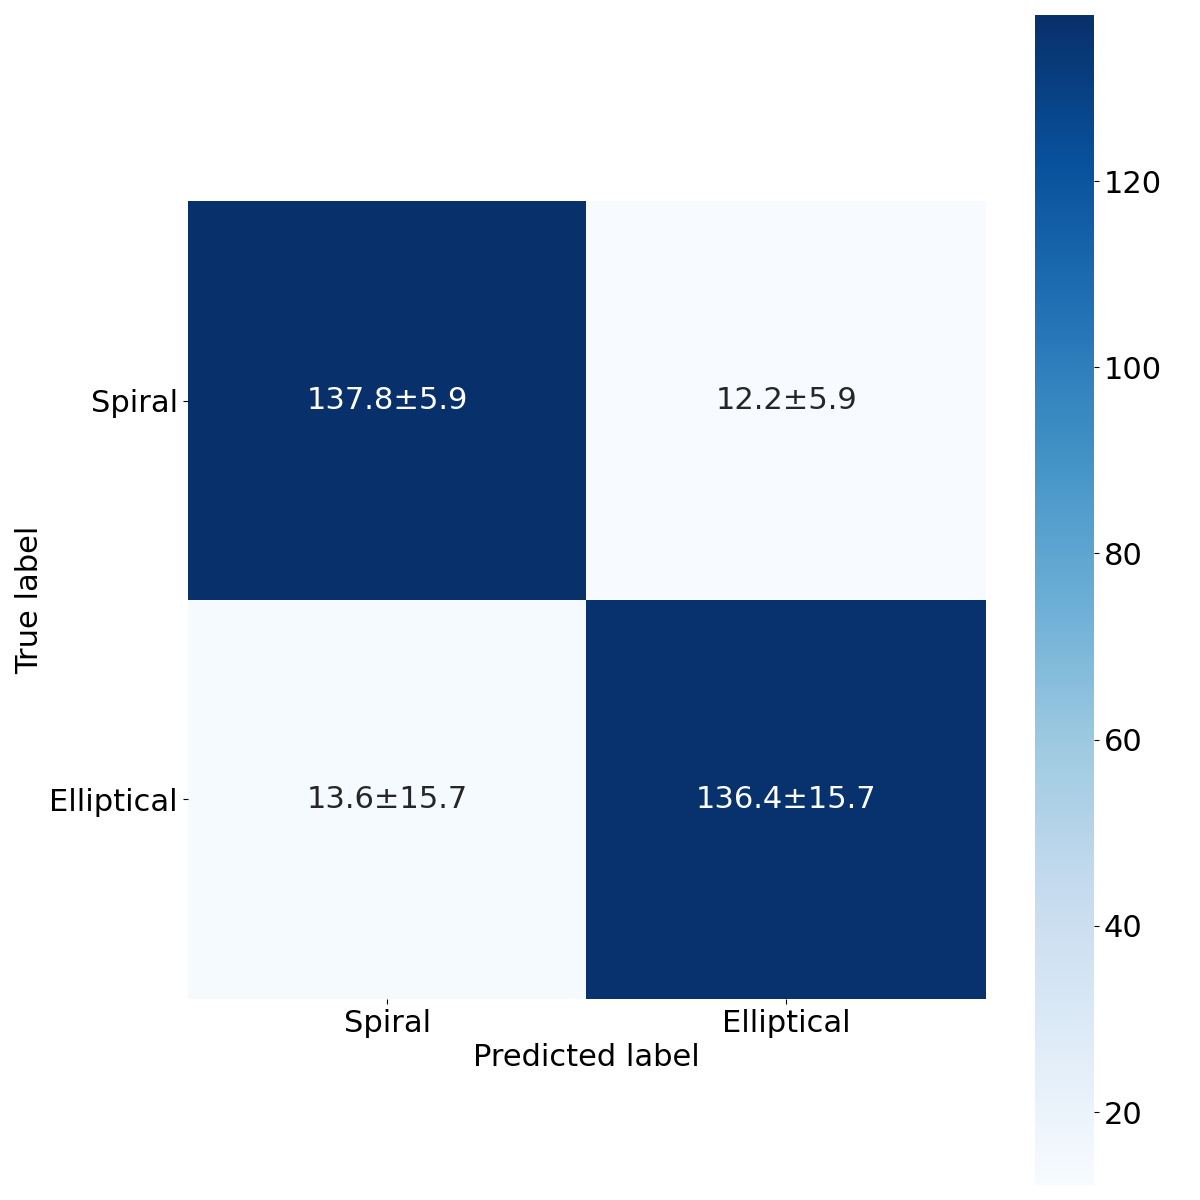
\includegraphics[keepaspectratio, width=7cm]{images/cm_mean_std_ex4-3.png}
    \caption{バランスドデータ : 混同行列\\(平均$\pm$標準偏差(1$\sigma$))}
		\label{fig:cm_ex4-3}
  \end{minipage}
\end{figure}


% \subsubsection{モデル学習の進行}
% 図\ref{fig:losses_ex4-2-2}・図\ref{fig:accs_ex4-2-2}において,テストデータに対するスコアが100epoch付近までloss関数は降下,accuracyは上昇するものの,それ以降のepochではloss関数は上昇するがaccuracyは横ばいになっている.このことから,インバランスドデータで学習を行ったモデルは100epoch目以降学習データに対し過適合はしているものの,テストデータに対する汎化性能は失っていないことが読み取れる.

% また図\ref{fig:losses_ex4-3}・図\ref{fig:accs_ex4-3}において,テストデータに対するスコアが75epoch付近までloss関数は降下,accuracyは上昇するものの,それ以降のepochではloss関数は上昇するがaccuracyは横ばいになっている.このことから,バランスドデータで学習を行ったモデルは75epoch目以降学習データに対し過適合はしているものの,テストデータに対する汎化性能は失っていないことが読み取れる.

\subsubsection{テストデータに対するaccuracyの評価}
モデルの形態分類性能を評価するため,両モデル間にてテストデータに対する予測のaccuracyの比較を行う.性能評価においては,4.2節同様,モデルが学習しきった際の分類性能を用いた.

両モデルにおける,テストデータへの予測精度(accuracy)を表\ref{tb:accs_4.3}に示す.表\ref{tb:accs_4.3}は4.2節における表\ref{tb:accs_4.2}と同様の形式であり,今回の30回実行におけるaccuracyの平均値と標準偏差をそれぞれ1$\sigma$分記載した.表\ref{tb:accs_4.3}より,テストデータに対する予測のaccuracyの標準偏差付き平均値において両モデル間で有意な差はなかった.

\subsubsection{TSSの導出方法,および両分類モデルの分類性能評価}
次に,データセット内のクラスインバランスに左右されづらい評価指標であるTSSにて,再度両モデルの評価・性能比較を行う.

% TSSを導出するため,先ほど求めた「モデルが学習しきった地点と思われる,テストデータに対するaccuracyが最大となるepoch数」まで,再度30回学習およびテストを両モデルにて行った.今回行ったこの再度30回学習およびテストをした結果は,後ほど混同行列の導出にも用いる.

両モデルのテストデータへの予測精度(TSS)を表\ref{tb:TSS_4.3}に示す.
表\ref{tb:TSS_4.3}より,標準偏差付き平均値を見たとき,TSSが両モデルとも0.8付近と高いスコアを記録しており,また両モデルにおける有意差はなかった.
TSSは両クラスの分類性能がどちらも高くないと数値が向上しない評価指標のため,
両モデルとも片方のクラスについて分類する性能が高いモデルではなく,両クラスへの分類性能をもつ分類モデルであることが分かる.

\subsubsection{混同行列によるモデルの評価}
最後に,混同行列を用いて各モデルのテストデータに対する予測精度の比較を行う.導出された混同行列をそれぞれ図\ref{fig:cm_ex4-2-2},図\ref{fig:cm_ex4-3}に示す.

図\ref{fig:cm_ex4-2-2}より,インバランスドデータを用いて学習およびテストを行ったモデルにおいて陽性を渦巻銀河とした場合のtrue positive rateは$215.0/(215.0+11.7) = 0.948$,楕円銀河とした場合は$61.7/(11.6+61.7) = 0.842$であることが分かる.
また図\ref{fig:cm_ex4-3}より,バランスドデータを用いて学習およびテストを行ったモデルにおいて陽性を渦巻銀河とした場合のtrue positive rateは$137.8/(137.8+12.2) = 0.919$,楕円銀河とした場合は$136.4/(13.6+136.4) = 0.909$であることが分かる.
2つのモデルを比較すると,インバランスドデータモデルは楕円銀河のtrue positive rateが0.9以下であるのに対し,バランスドデータは両クラスのtrue positive rateが0.9以上であることが分かる.このことから,インバランスドデータモデルは渦巻銀河のデータ数が多い分,渦巻銀河を渦巻銀河と分類する能力が高く,またバランスドデータモデルは渦巻銀河を渦巻銀河と,楕円銀河を楕円銀河と分類する能力が同程度に高いモデルであることが分かる.

% \begin{table}[htbp]
%   \centering
% 	\caption{インバランスドデータで学習を行ったモデル,およびバランスドデータで学習を行ったモデルのテストデータに対する予測のaccuracy}
%   \begin{tabular}{|c|c|c|}
% 		\hline
%     & mean$\pm$std (2$\sigma$) & mean$\pm$ste (2$\sigma$) \\ \hline
%     インバランスドデータでのモデル & $0.931 \pm 0.034$(158th epoch) & $0.931 \pm 0.006$(158th epoch) \\ \hline
%     バランスドデータでのモデル & $0.922 \pm 0.036$(123th epoch) & $0.922 \pm 0.007$(123th epoch) \\ \hline
%   \end{tabular}
%   \label{tb:accs_4.3}
% \end{table}

\begin{table}[H]
  \centering
	\caption{ラベルインバランスによるaccuracyの変化}
  \begin{tabular}{|c|c|}
		\hline
    & mean (1std) \\ \hline
    インバランスドデータでのモデル & $0.931 \pm 0.017$(158th epoch) \\ \hline
    バランスドデータでのモデル & $0.922 \pm 0.018$(123th epoch) \\ \hline
  \end{tabular}
  \label{tb:accs_4.3}
\end{table}

% \begin{table}[htbp]
%   \centering
% 	\caption{インバランスドデータで学習を行ったモデル,およびバランスドデータで学習を行ったモデルのテストデータに対する予測のTSS}
%   \begin{tabular}{|c|c|c|}
% 		\hline
%     & mean$\pm$std (2$\sigma$) & mean$\pm$ste (2$\sigma$) \\ \hline
%     インバランスドデータでのモデル & $0.791 \pm 0.250$ & $0.791 \pm 0.046$ \\ \hline
%     バランスドデータでのモデル & $0.828 \pm 0.184$ & $0.828 \pm 0.033$ \\ \hline
%   \end{tabular}
%   \label{tb:TSS_4.3}
% \end{table}

\begin{table}[H]
  \centering
	\caption{ラベルインバランスによるTSSの変化}
  \begin{tabular}{|c|c|}
		\hline
    & mean (1std) \\ \hline
    インバランスドデータでのモデル & $0.791 \pm 0.125$ \\ \hline
    バランスドデータでのモデル & $0.828 \pm 0.092$ \\ \hline
  \end{tabular}
  \label{tb:TSS_4.3}
\end{table}

\newpage
\section{議論}
4.2節では,不確かな天体とラベル付けされている天体をモデル学習およびテストに用いた際の分類精度への影響を調べるため,不確かな天体を使用したモデルと除外したモデルを作成し,両モデルの比較を行った.
その結果,4.2節の実験にて不確かな天体を入れた3値分類問題とした方がテストデータに対する予測精度が落ちてしまう現象が確認された.
この現象には2つの可能性が考えられる.1つ目は,GZの形態分類フラグで不確かな天体と判定された天体が実際は渦巻銀河であったり楕円銀河である可能性である.GZの形態分類フラグは,渦巻銀河および楕円銀河の投票率が0.8である場合に渦巻および楕円というフラグが立ち,それ以外の場合は不確かな天体にフラグが立つ.渦巻および楕円と不確かな天体は0.8という閾値で区切られているが,この閾値では渦巻銀河および楕円銀河が不確かな天体とフラグ付けされている可能性がある.このようにクラスのラベル付けが間違っているデータをモデルに用いた場合,モデルの学習は問題なく進むが,テストデータへの分類精度は低下する.
2つ目は,GZの形態分類フラグにて星もしくは分からない天体とマージャーが全て不確かな天体と判定されるため,不確かな天体クラスの天体種類に多様性が存在する可能性である.GZの形態分類フラグでは,星もしくは分からない天体とマージャーの投票率が最も高い天体には不確かな天体と判定されている.このため,不確かな天体クラスは,実際には人間による判定の信頼度が低い(すなわち0.8の投票率に届かなかった)渦巻銀河および楕円銀河・星もしくは分からない天体・マージャーの4つが混在していると考えられる.この不確かな天体クラス内の天体種類の多様性が,モデルの不確かな天体についての学習を難しくしており,結果としてテストデータに対する予測精度が低下する可能性がある.


4.3節では,使用する天体の銀河形態ラベルのクラスインバランスがモデルの分類精度に与える影響を調べるため,渦巻銀河と楕円銀河の比率が異なるインバランスデータを用いたモデルと,比率を等しくしたバランスドデータを用いたモデルを作成し,両モデルの比較を行った.
その結果,4.3節の実験にて学習・テストに用いるデータ内のクラスインバランス改善を行っても分類精度の改善が見受けられなかった.このことから,今回の実験で見受けられたようなクラスインバランスでは,分類精度への影響は小さい可能性がある.もしデータセット内に桁数が異なるほどのクラスインバランスが起きていた場合,インバランスを改善せずにモデル作成を行った場合,分類精度に悪影響が発生する可能性がある.
% もし学習データ内にて桁数が異なるほどの強いデータインバランスが起きていた場合,データインバランス改善を行えば分類精度が改善される可能性がある.

4章の目標は学習データとテストデータの解像度が揃っているという条件のもと,どの程度の精度の分類モデルを作成することができるかを確認することであり,そのために2つの実験を行った.GZにて不確かと分類されている天体を除外し,渦巻銀河・楕円銀河の2値分類問題とすることで,分類モデルの分類精度は大きく向上した.一方で,学習・テストに用いるデータ内のデータインバランスを改善しても分類精度に有意差が認められるほどの向上は見受けられなかった.本研究における今後の実験では,渦巻銀河を分類することに特化したモデルでなく,渦巻銀河・楕円銀河の両者を分類することを優先するため,渦巻銀河・楕円銀河のtrue positive rateがある程度等しくなることが見込めるバランスドデータにてモデル学習を行っていく.



\newpage
\chapter{空間解像度差のあるデータセットを用いた分類モデル作成}
% 本研究の将来展望は,高空間分解能観測装置データを用いてモデル学習を行うことで,既存の低空間分解能データセットに対し更なる高精度形態分類を提供するというものである.この将来展望の前提条件である,学習データとテストデータとの間の解像度が揃っているデータセットにて高精度の銀河形態分類モデルを学習させることを,第4章にて達成することができた.

% そこで,
この章では
% 将来展望で行われる予定の
異なる観測装置データの組み合わせを念頭に置き,学習データとテストデータとの間に解像度差があるデータセットにて形態分類モデルの作成が行えるかを検証する.

\section{実験概要}
第5章ではSDSSから取得した銀河切り出し画像とGZから取得した分類フラグを学習データとしてモデルを学習させ,銀河切り出し画像を縮小した低解像度データセットに対し予測を行う.なお,学習・テストに用いる天体データの銀河種は渦巻銀河・楕円銀河の2つとする.

\subsubsection{学習データ}
学習データには第4章で用いた14,998天体のうち不確かな天体を除いた,渦巻銀河4,057天体,楕円銀河は1,561天体の計5,618天体を用いた.

\subsubsection{縮小画像データセット(テストデータ)の作成方法}
この章ではテストデータとして,SDSSから取得した銀河切り出し画像を縮小したデータセットを使用する.学習データにも用いている5,618天体を,平均画素法により縮小処理を施した.平均画素法とは画像処理法の一つであり,縮小前画像と縮小画像の画像サイズの面積比を用いて,画像の縮小を行う方法である.画像の縮小にはOpenCVに実装されているresize関数のINTER\_AREAメソッドを使用した.ここでresize関数は画像の拡大または縮小を行う関数であり,INTER\_AREAメソッドとは平均画素法による画像補間処理を行うメソッドである.
銀河切り出し画像を1/2, 1/3, ..., 1/7, 1/8倍に縮小し,計7つの縮小画像データセットを作成した.縮小画像の例として,1/4倍に縮小した画像群を図\ref{fig:shrink_1_4}に示す.

\begin{figure}
 \centering
 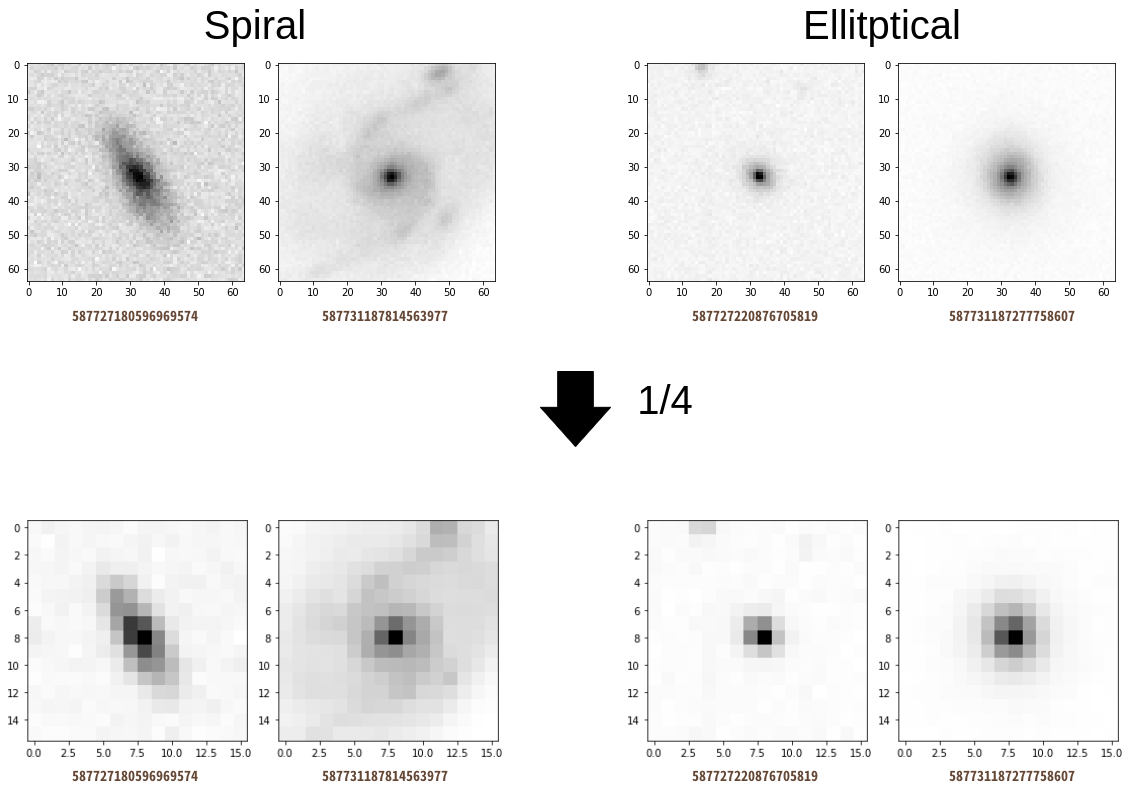
\includegraphics[width=13cm]{images/5syou/syuron_5syou_kakudai/ver1/5syou_shrink_ver1.png}
 \caption{銀河切り出し画像の縮小例(1/4倍)}
 \label{fig:shrink_1_4}
\end{figure}

\subsubsection{縮小画像データセットの拡大方法}
モデルに画像データを入力する際,用いる画像サイズは揃えて入力する必要があり,今回の実験条件では学習データである高解像度データの画像サイズへ揃える必要がある.
そのため,今回の実験ではテストデータである縮小画像データセットを拡大してモデルに入力する.

縮小画像の拡大には,OpenCVのresize関数を用いた.この章での実験において,画像拡大の際の補間方法として最近傍補間,バイリニア補間,バイキュービック補間を使用した.画像拡大の例として,1/4倍に縮小された銀河切り出し画像の,各補間方法による画像拡大の例を図\ref{fig:kakudai_1_4}に示す.なお図\ref{fig:kakudai_1_4}にて用いられている縮小画像は,図\ref{fig:shrink_1_4}のものと同様である.

\begin{figure}[H]
 \centering
 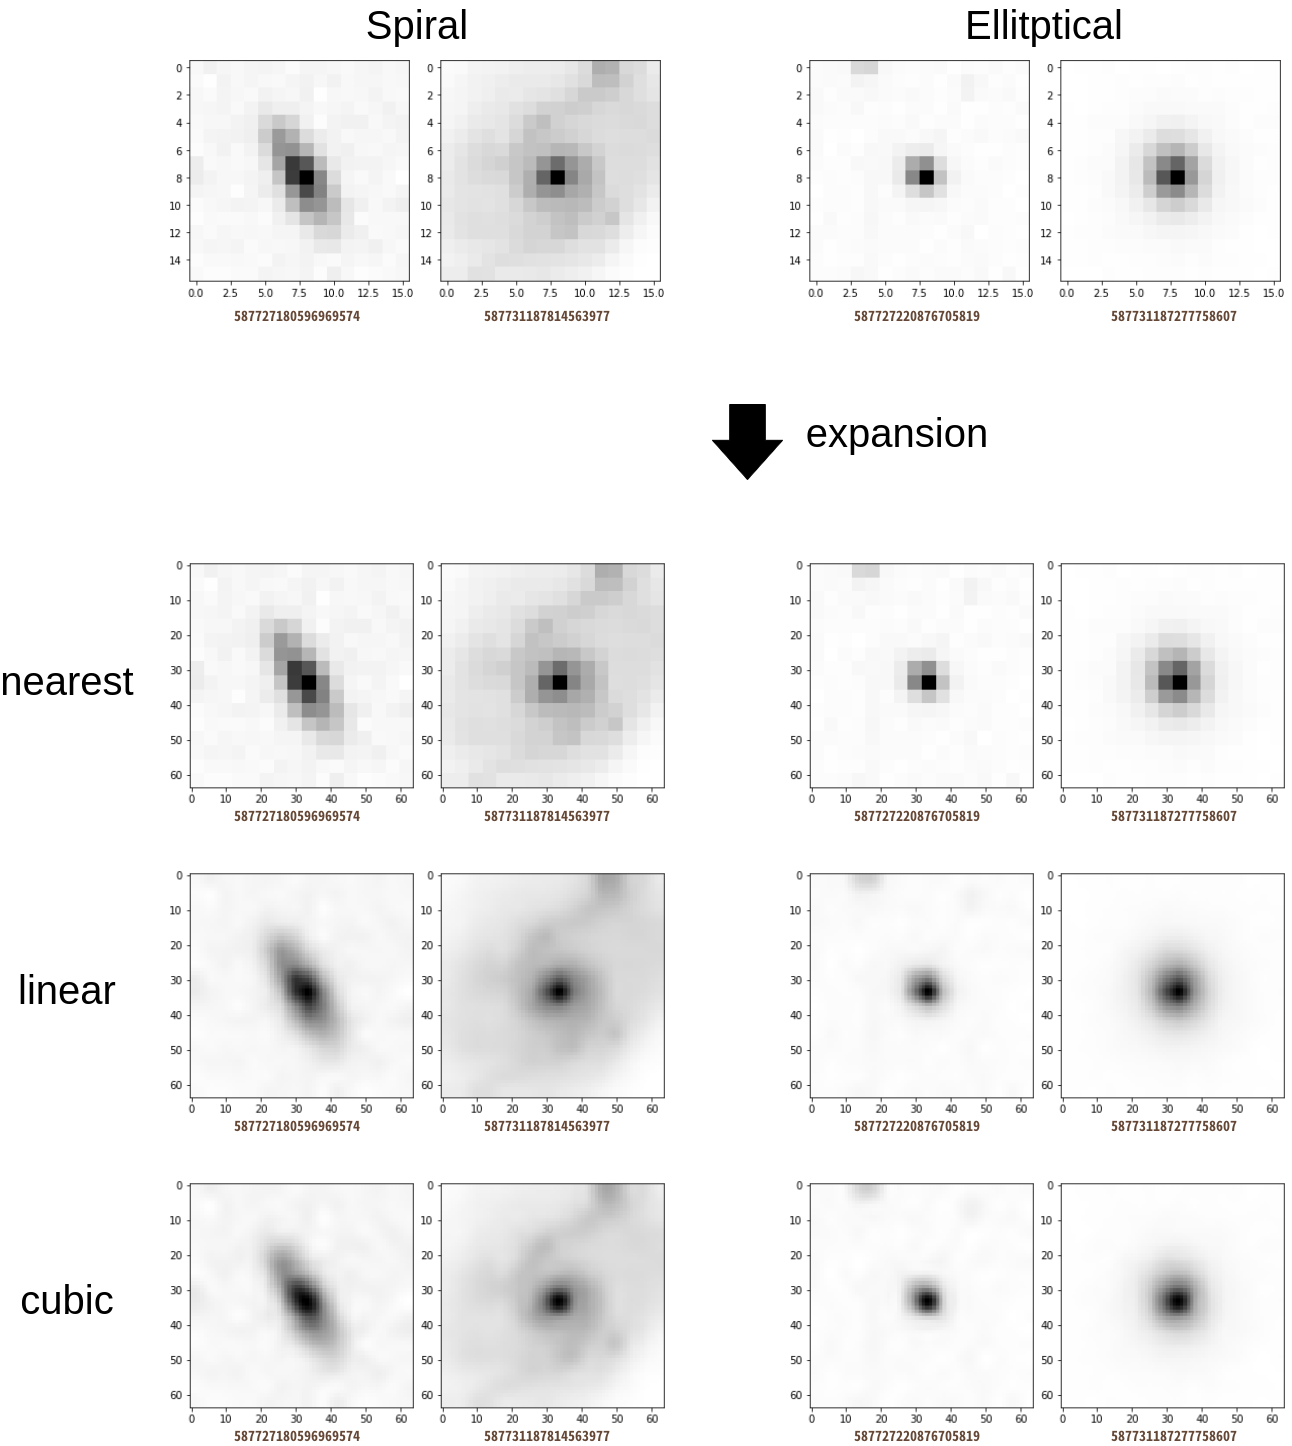
\includegraphics[width=13cm]{images/5syou/syuron_5syou_kakudai/ver1/5syou_kakudai_ver1.png}
 \caption{1/4倍縮小画像の画像拡大例//(最近傍補間・バイリニア補間・バイキュービック補間)}
 \label{fig:kakudai_1_4}
\end{figure}

\subsubsection{モデル構造}
今回用いた深層学習モデルは,cheng et al.(2019)\cite{Cheng2019}にて用いられていた銀河形態分類モデルを参考にした.今回用いたモデルの構造を図\ref{fig:model_shape_2}に示す.このモデルは畳み込み層を合計3つ有しており,それぞれのカーネルサイズは3x3, 3x3, 2x2である.それぞれの畳み込み層の後には,2x2のmax-pooling層が存在する.全畳み込み層の後に全結合層が2層配置されており,それぞれ1024個のノードを有している.

\begin{figure}[h]
	\centering
	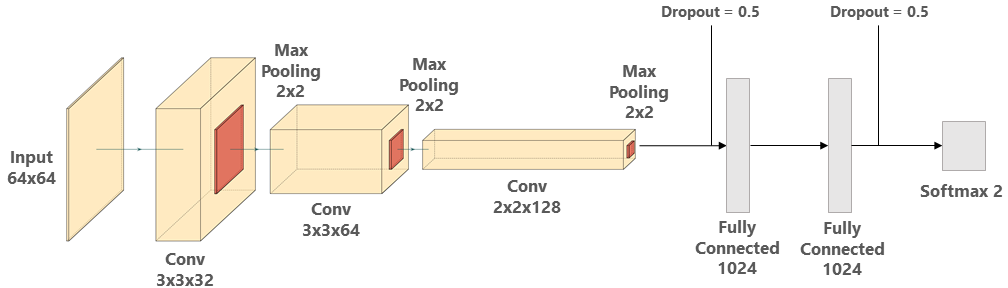
\includegraphics[width=14cm]{images/model_shape.png}
	\caption{用いた分類モデルの構造図}
	\label{fig:model_shape_2}
\end{figure}
 
\subsubsection{モデルの評価方法}
分類モデルの評価指標として,accuracy (正解率)を用いた.accuracyは全テストデータの中で正しく分類できたデータがどれだけあるかというものであり,モデルの正確性を表す指標である.

また,深層学習モデルには実行毎に学習のブレが存在するため,モデルの評価の際には学習・テストを30回実行し,評価指標の平均値,標準偏差および標準誤差を導出する.

\section{分類精度のデータセット内解像度差依存性}
この節では,学習データとテストデータとの間に解像度差がある状況において,
\begin{inparaenum}[(1)]
  \item テストデータへの予測が成立するか
  \item 予測が成立する場合,解像度差がいくつまでならば使用可能か
\end{inparaenum}
の検証を行う.このうち(2)において「使用可能」の定義として,学習データとテストデータの解像度が揃っている状況での予測結果である''Original''と同程度の高精度な分類,すなわちaccuracyが0.9付近を記録する結果であることとする.

\subsection{実験条件}
使用する天体は,GZによる形態分類が行われた15,000天体(図\ref{fig:z_15000}参照)を母集団とした.銀河種類ごとのデータインバランスが起こらないようにするため,その母集団の中から渦巻銀河と楕円銀河をそれぞれ300天体選定した.選定を行う際,赤方偏移$z$について,$0 < z < 0.2$という条件を設定し,あてはまらない天体は除外を行う.これは,地球との距離が遠すぎる天体については上手く特徴抽出が行えず学習の妨げになる可能性があるからである.

使用天体を渦巻銀河300天体,楕円銀河300天体の合計600天体を選定したあと,学習データとテストデータの比率が7:3となるように天体群を分けた.このうち,学習データにはSDSSの切り出し画像,テストデータにはSDSSの切り出し画像を縮小した画像をそれぞれ用いた.また,学習データとテストデータ内において,銀河種のデータインバランスが起こらないようにするため,渦巻銀河と楕円銀河の比率が等しくなるようにした.

モデルの評価を行う際,モデルの学習およびテストを30回行い,accuracyの平均値,標準偏差および標準誤差を導出した.
なお,30回の学習およびテストの際,学習実行毎に使用される天体は毎回シャッフルされる.

モデルの学習期間は900epochとした.これは,すべての縮小データの縮小倍率にて,モデルが学習しきる期間,すなわちテストデータに対するaccuracyが上がりきるepoch数が900epochであったからである.

\subsection{実験結果}
\subsubsection{縮小データに対する予測結果}
銀河切り出し画像を1/2倍から1/8倍に縮小した縮小データに対する,形態分類モデルの予測結果の図を図\ref{fig:nearest_300_1std}から図\ref{fig:inter_comparison_300_1std}に示す.

\begin{quote}
 \begin{itemize}
  \item 横軸が,テストデータである縮小データの縮小倍率であり,縦軸がテストデータに対する予測のaccuracyとなっている.
  \begin{quote}
   \begin{itemize}
    \item テストデータに対する予測のaccuracyについて,30回実行における平均値と標準偏差(2std)をエラーバー形式で示している.
    \item なお,一番左に位置しているOriginalとなっている箇所は,テストデータに縮小データでなく,学習データと同じ大きさの銀河切り出し画像を使用してテストを行った結果である.すなわち,Originalが学習データとテストデータの解像度が揃っている状況での予測結果に対し,1/2から1/8が学習データとテストデータとの間に解像度差がある状況での予測結果を示している.
   \end{itemize}
  \end{quote}
  \item accuracyを採るepoch数は,モデルが十分に学習しきるepoch数とした.すなわち,テストデータに対するaccuracyが最大値となるepoch数とした.
  \item 図\ref{fig:inter_comparison_300_1std}には,内挿方法間でのaccuracyの比較を図に示した.
 \end{itemize}
\end{quote}

\begin{figure}[H]
 \centering
 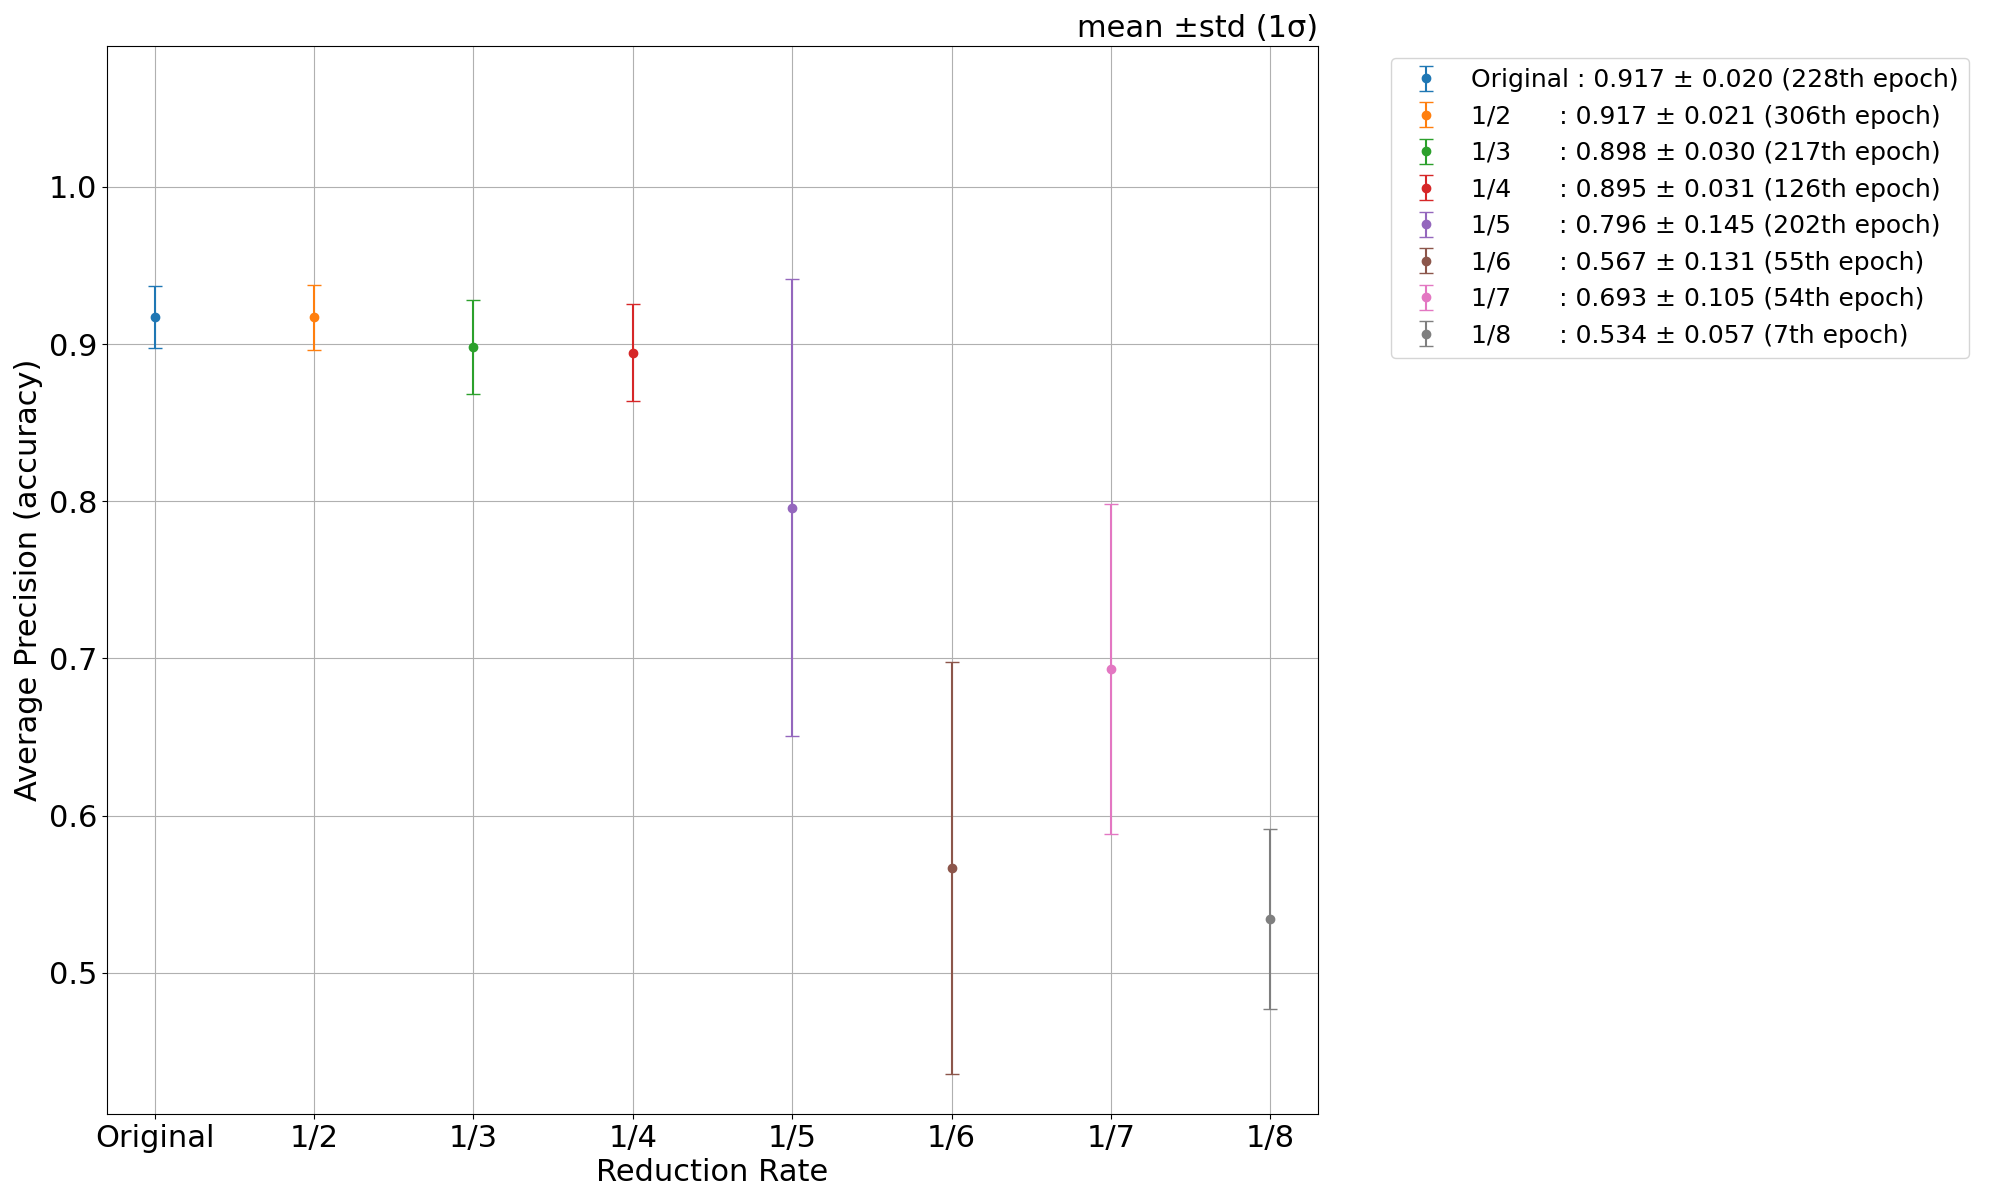
\includegraphics[width=16cm]{images/5syou/print_errorbar/nearest/acc_with_errorbar_syuron5_nearest_900epoch_30run_300_acc_max_std1sigma.png}
 \caption{最近傍補間によって内挿された,縮小データに対するモデルの予測結果(1std)}
 \label{fig:nearest_300_1std}
\end{figure}

\begin{figure}[H]
  \centering
  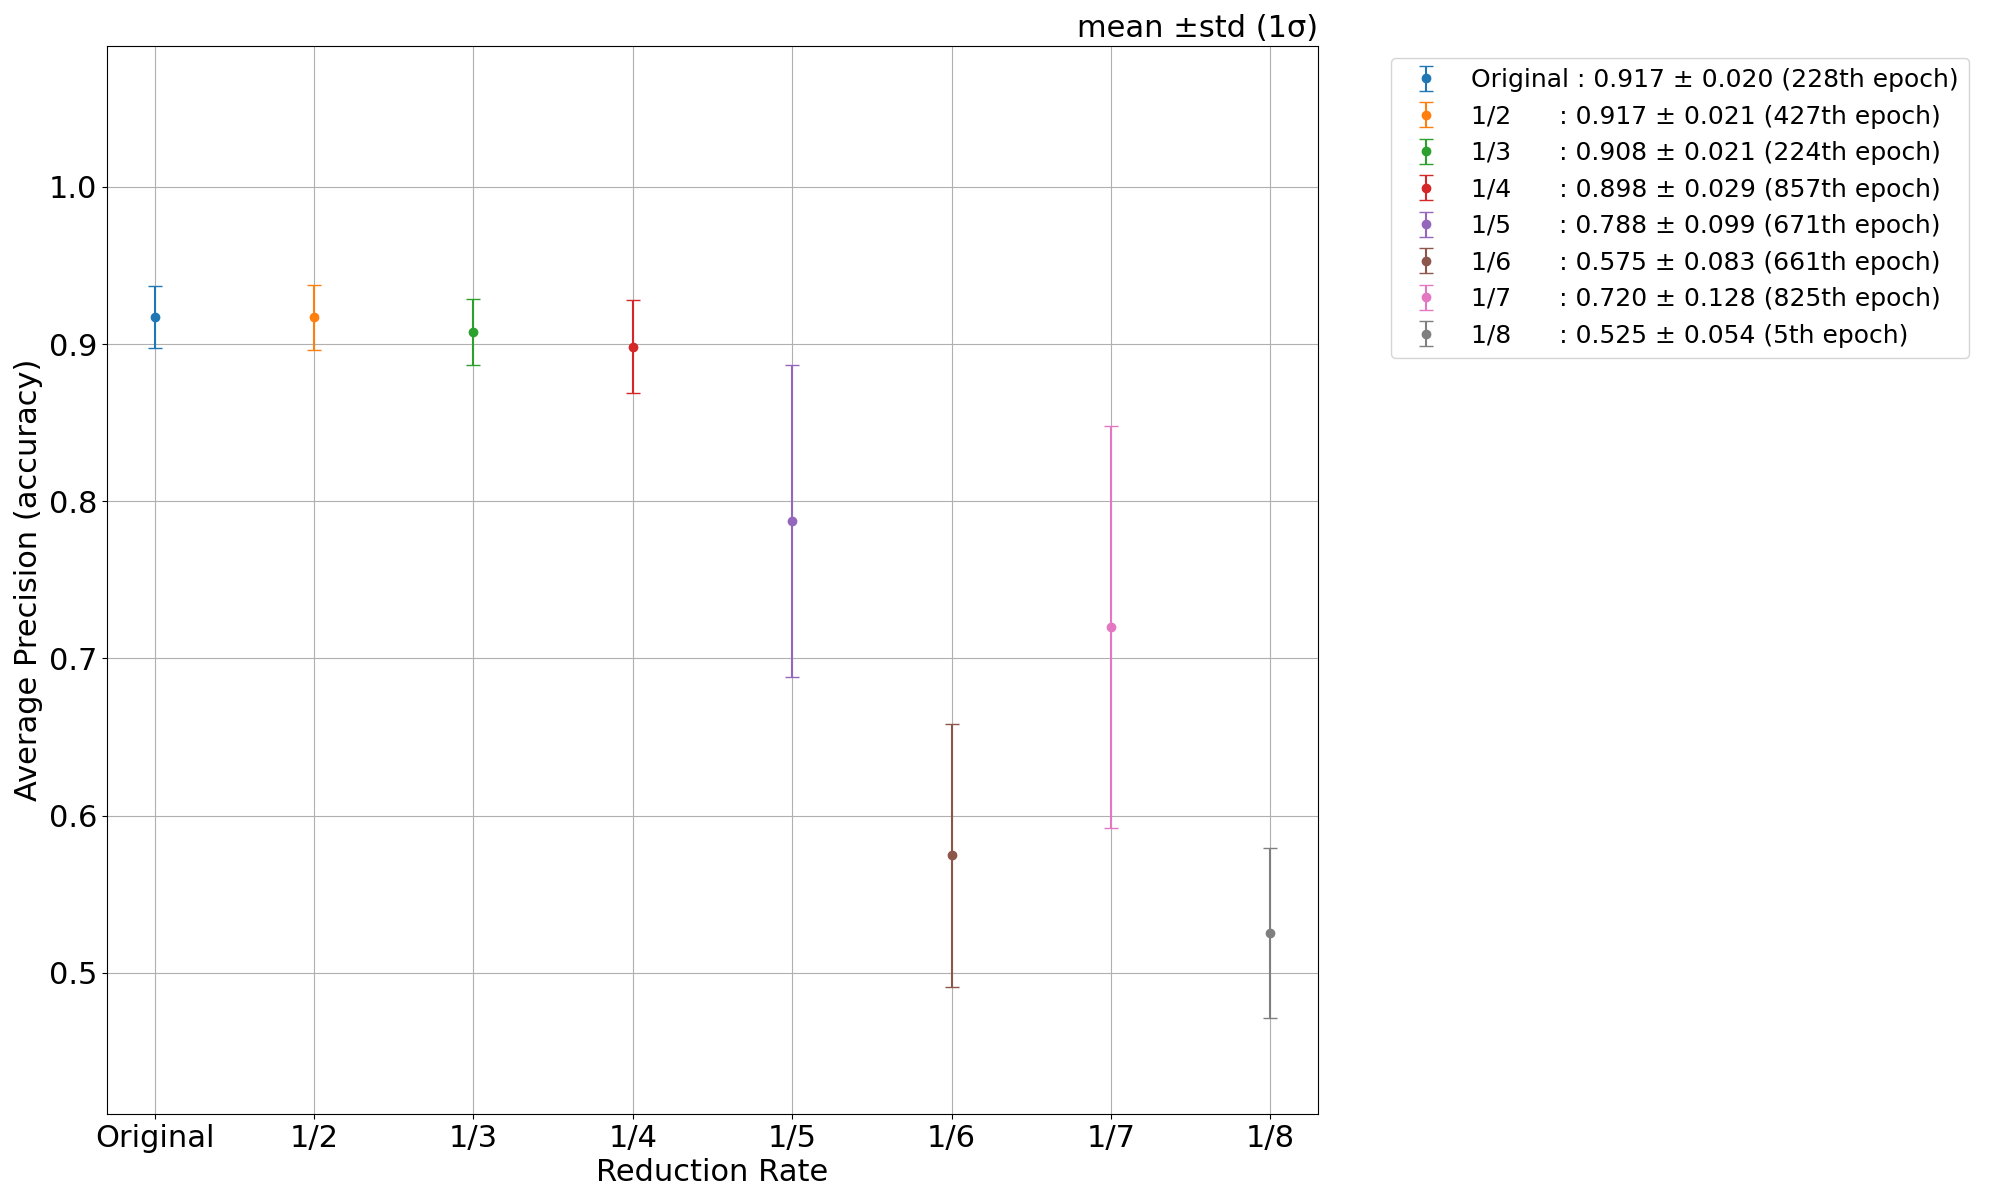
\includegraphics[width=16cm]{images/5syou/print_errorbar/linear/acc_with_errorbar_syuron5_linear_900epoch_30run_300_acc_max_std1sigma.png}
  \caption{バイリニア補間によって内挿された,縮小データに対するモデルの予測結果(1std)}
  \label{fig:linear_300_1std}
\end{figure}

\begin{figure}[H]
  \centering
  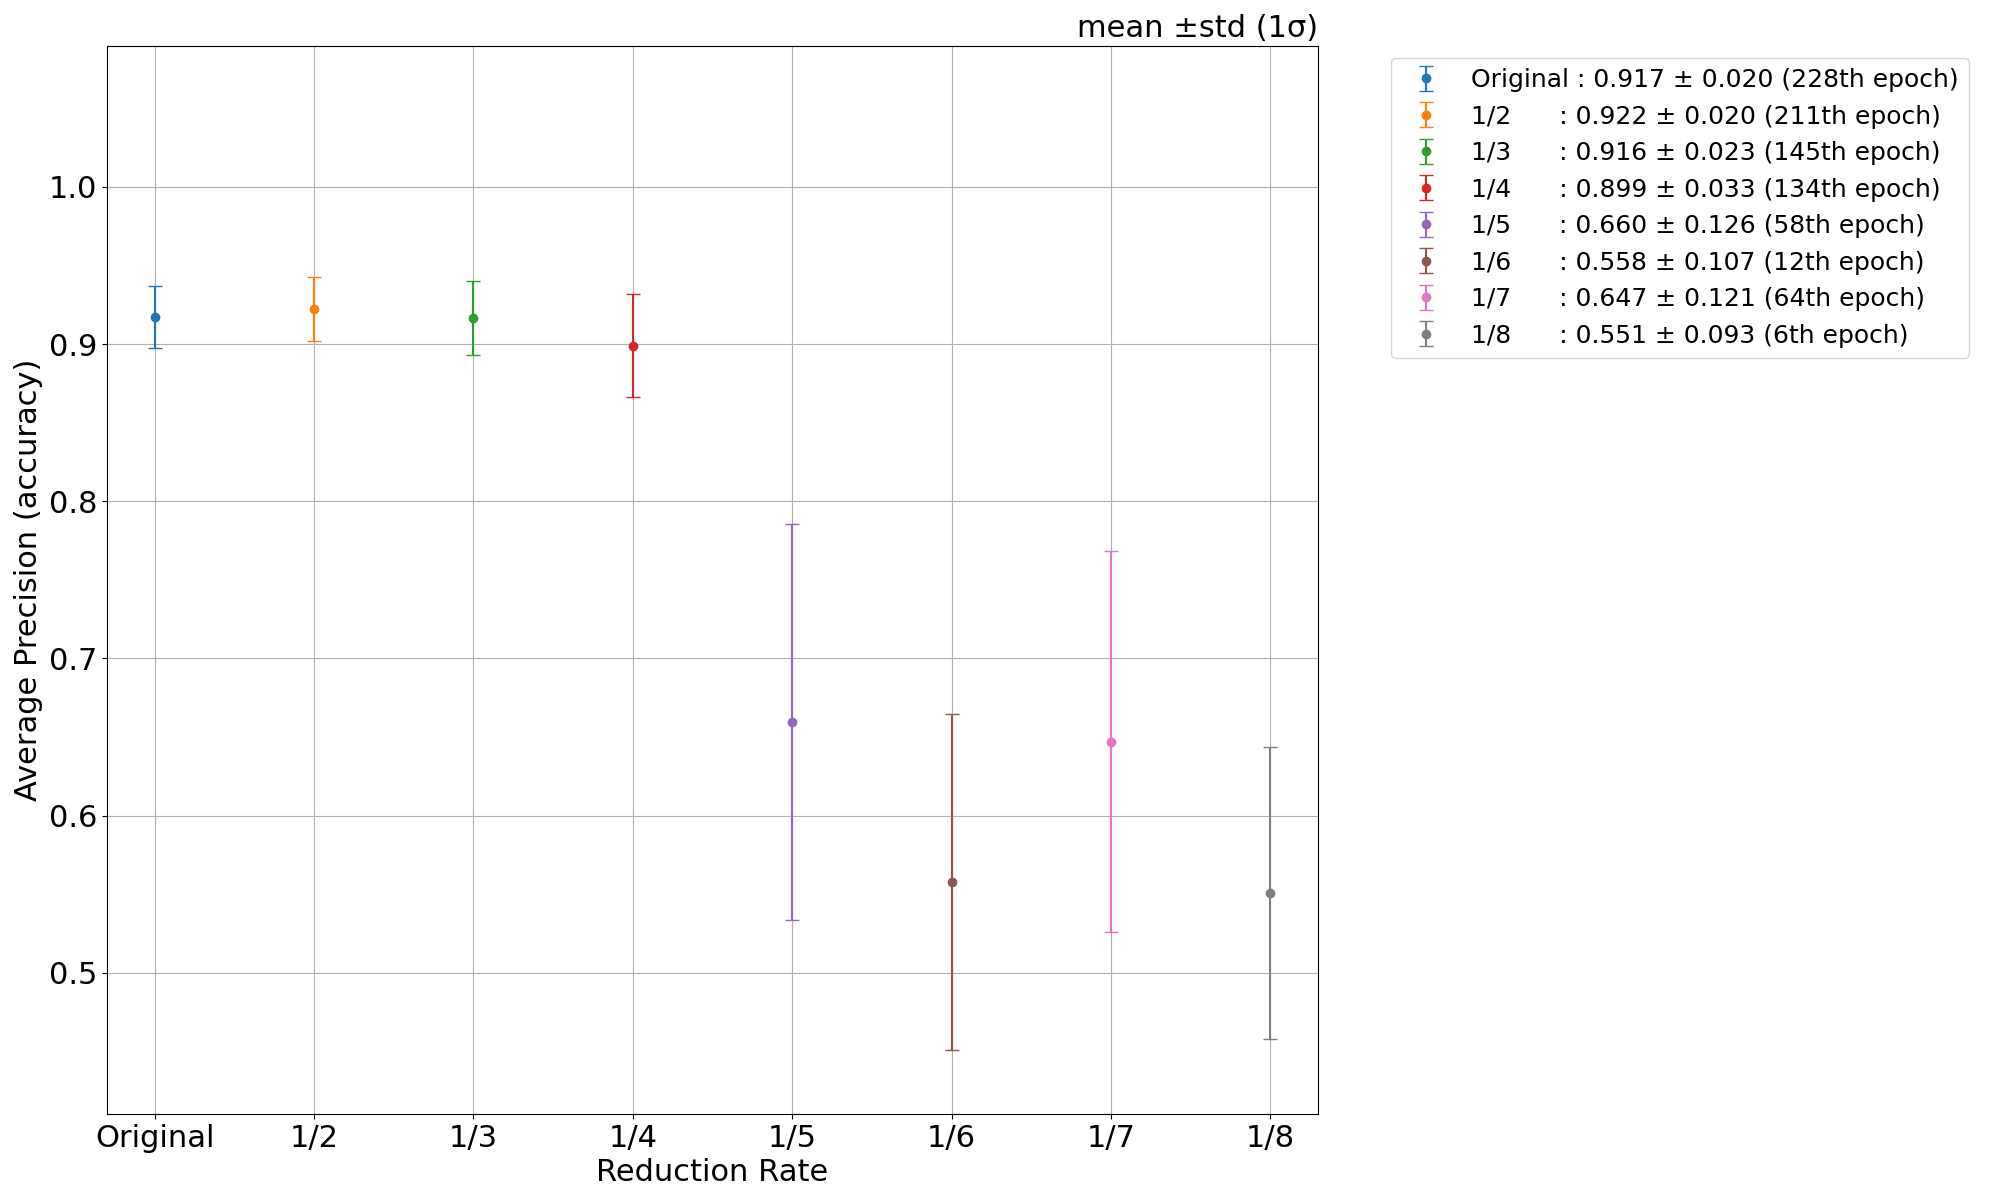
\includegraphics[width=16cm]{images/5syou/print_errorbar/cubic/acc_with_errorbar_syuron5_cubic_900epoch_30run_300_acc_max_std1sigma.png}
  \caption{バイキュービック補間によって内挿された,縮小データに対するモデルの予測結果(1std)}
  \label{fig:cubic_300_1std}
\end{figure}

\begin{figure}[H]
  \centering
  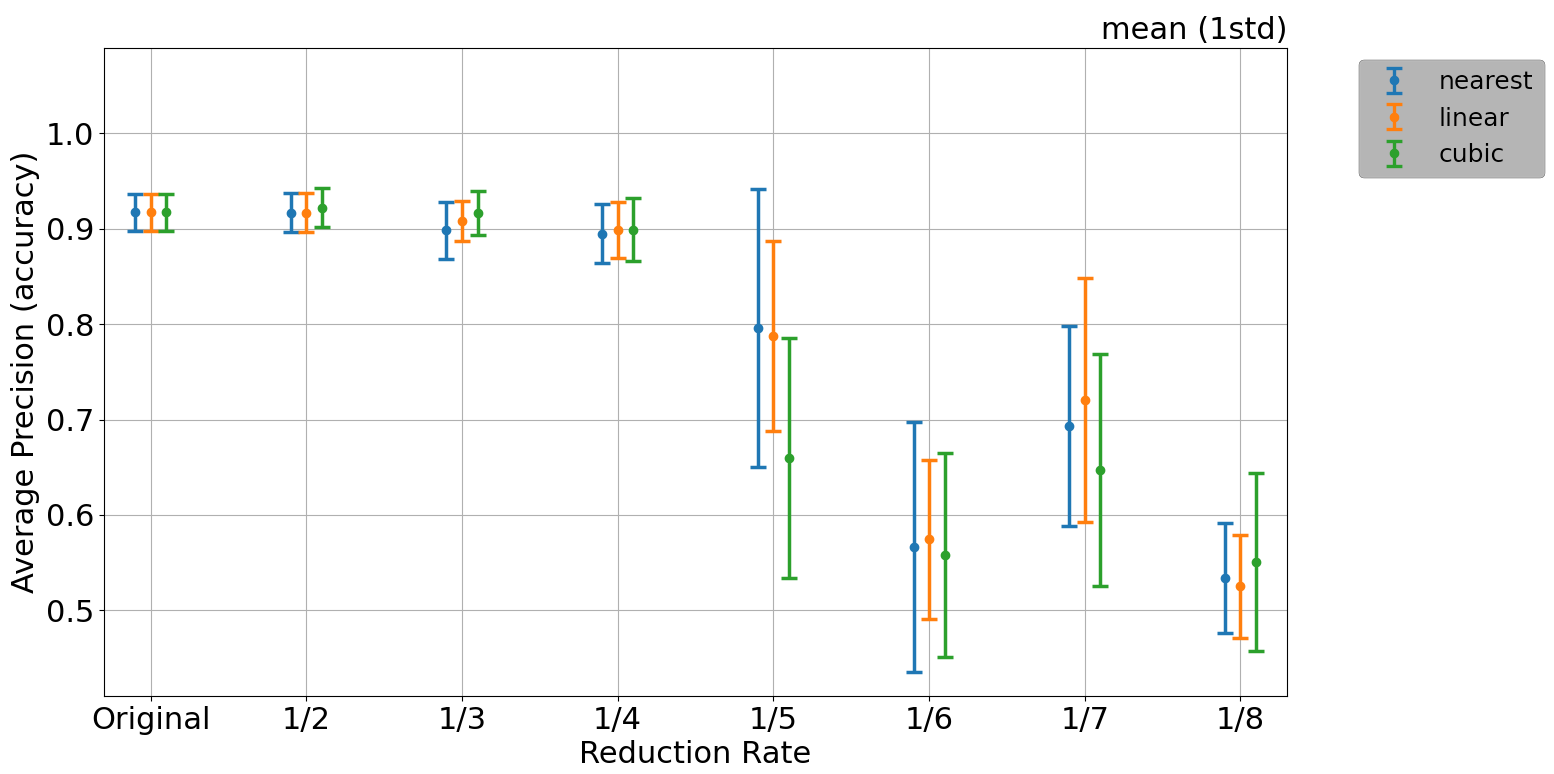
\includegraphics[width=16cm]{images/5syou/print_errorbar/print_errorbar_inter_comparison/acc_with_errorbar_syuron5_inter_comparison_900epoch_30run_300_acc_max_std1sigma.png}
  \caption{内挿方法間での比較(1std)}
  \label{fig:inter_comparison_300_1std}
\end{figure}


\subsubsection{結果}
\subsubsection{縮小データの縮小倍率における結果}
図\ref{fig:nearest_300_1std},図\ref{fig:linear_300_1std},図\ref{fig:cubic_300_1std}より,Originalの結果(学習データとテストデータの解像度が揃っている状況での予測結果)と同程度かつaccuracyが0.9付近を記録しているテストデータの縮小倍率が存在することが分かる.

図\ref{fig:nearest_300_1std}より,最近傍補間によって拡大したテストデータに対する予測は,縮小倍率が1/2から1/4倍の縮小データに対しては使用可能であることが分かる.なお,縮小倍率が1/5倍の縮小データに対する予測においては,accuracyが0.9を記録するモデルは1標準偏差区間において上位約17\%程しかなく,モデルの学習にかなりの上振れが起こらないと達成できないスコアであることから,使用可能ではないとの判断を行った.

同様に,図\ref{fig:linear_300_1std}よりバイリニア補間によって拡大したテストデータに対する予測は,縮小倍率が1/2から1/4倍の縮小データに対しては使用可能であり,また図\ref{fig:cubic_300_1std}よりバイキュービック補間によって拡大したテストデータに対する予測は,縮小倍率が1/2から1/4倍の縮小データに対しては使用可能であることが分かる.\\このことから,内挿方法によらず,学習データとテストデータの解像度差が1/4倍までであったら,テストデータとして使用可能であることが分かった.

\subsubsection{内挿方法間での比較}
内挿方法の間で,テストデータに対するaccuracyの細かい挙動を比較する.図\ref{fig:inter_comparison_300_1std}より,1/2から1/4倍,および1/6から1/8倍の縮小データにおいては,1標準偏差の誤差区間において内挿方法による有意差は見受けられない.また,1/5倍の縮小倍率においてはバイキュービック補間によって内挿したテストデータに対する予測のaccuracyが他2手法より劣って見えるが,1標準偏差の誤差区間においては他2手法との有意差は見られない.このことから,テストデータへの予測のaccuracyにおいて,テストデータの内挿方法における有意差はないことが分かった.

\subsubsection{標準誤差(1std)における予測結果}
図\ref{fig:nearest_300_1std}から図\ref{fig:cubic_300_1std}では,標準偏差(1std)を示した.ここで,標準誤差(1ste)の結果を図\ref{fig:nearest_300_1ste}から図\ref{fig:cubic_300_1ste}に示す.

1標準偏差(図\ref{fig:nearest_300_1std}から図\ref{fig:cubic_300_1std})と比べると,1標準誤差の誤差区間では各縮小倍率間で有意差が生じる.例として,図\ref{fig:nearest_300_1ste}を見ると,1標準偏差の誤差区間では有意差がなかった1/2倍と1/3倍の縮小データに対するaccuracyに,有意差が生じていることが読み取れる.このことから,深層学習において1つ1つのモデル学習にかなりのブレがあることがわかる.



\begin{figure}[H]
  \centering
  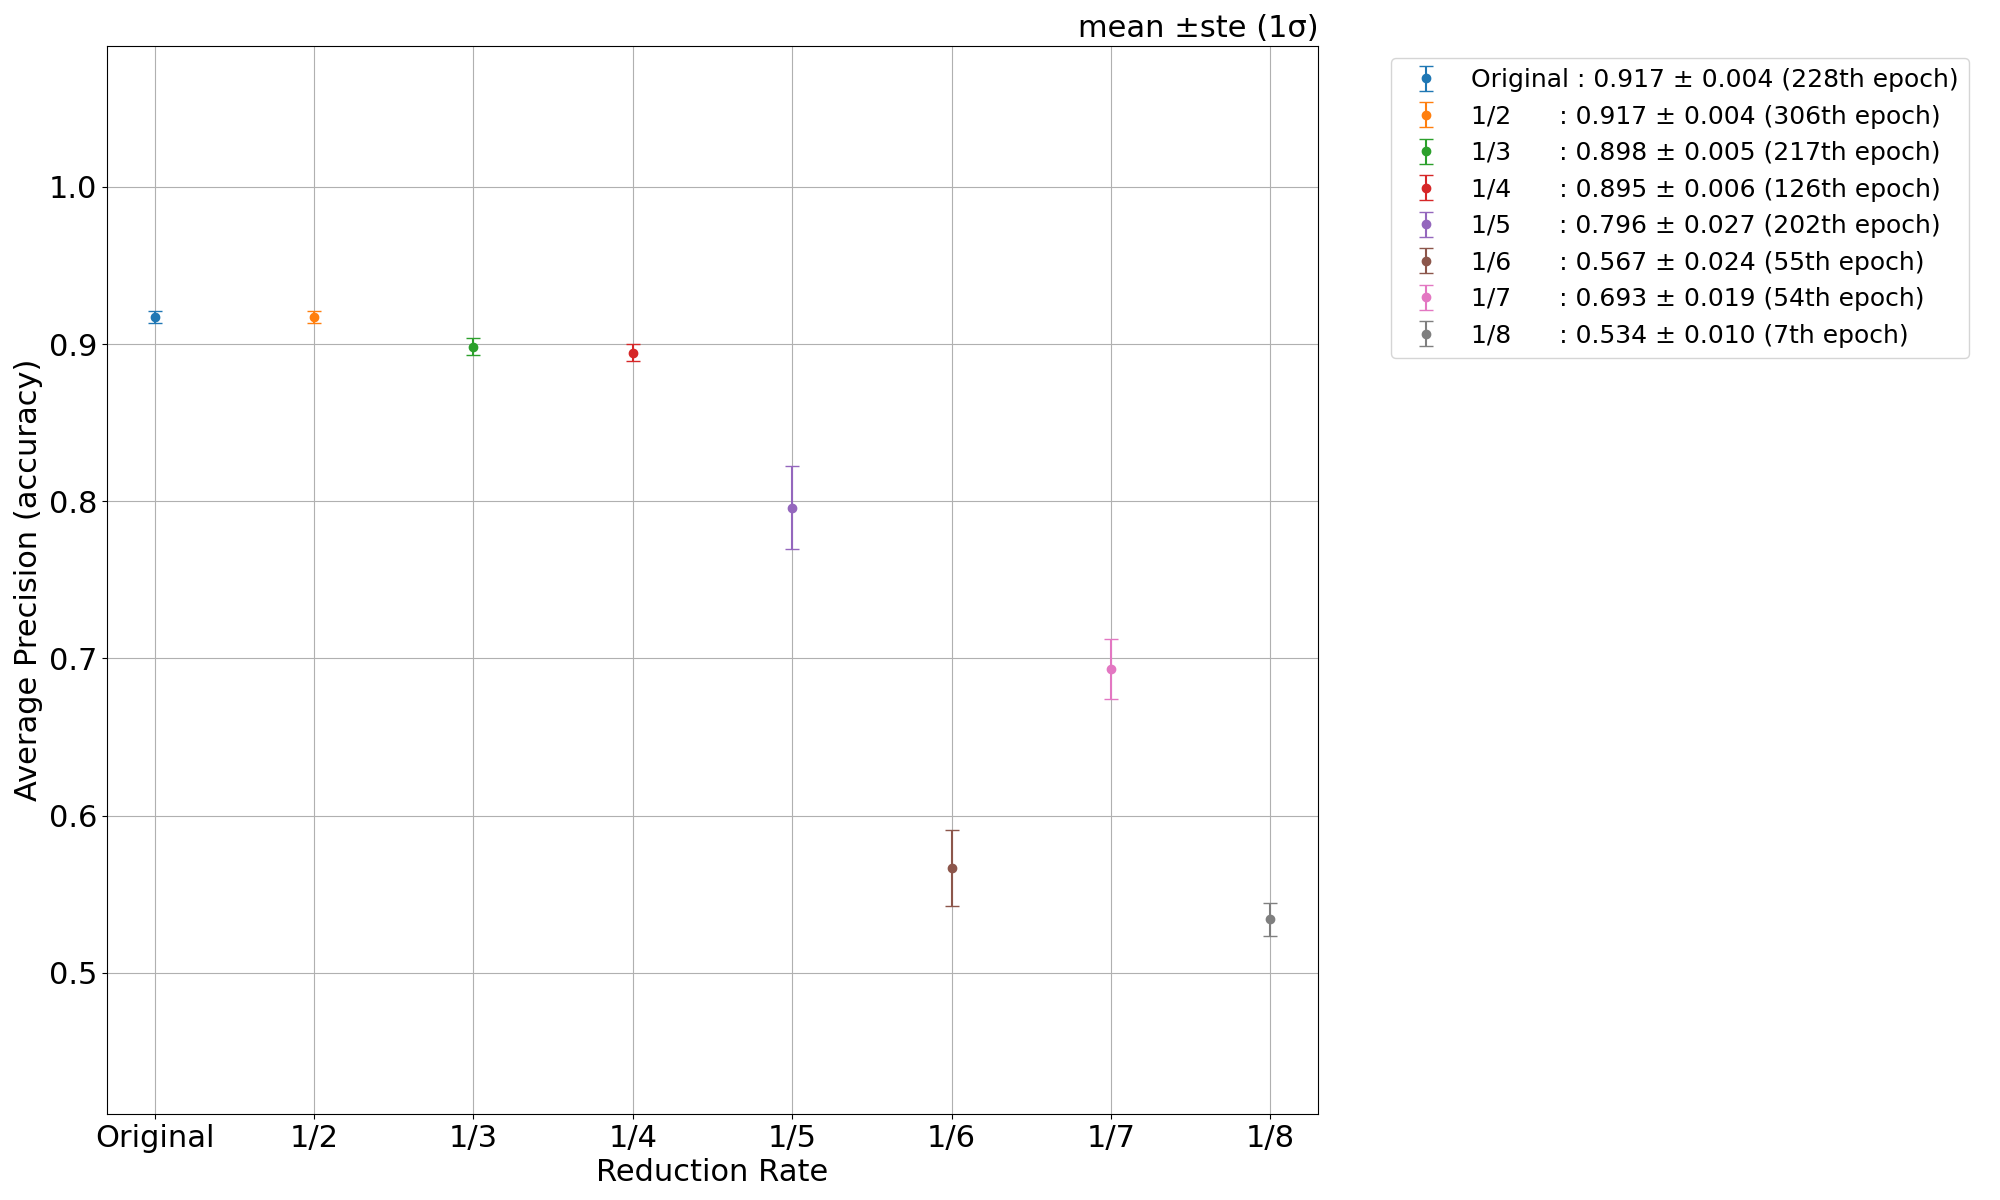
\includegraphics[width=16cm]{images/5syou/print_errorbar/nearest/acc_with_errorbar_syuron5_nearest_900epoch_30run_300_acc_max_ste1sigma.png}
  \caption{最近傍補間によって内挿された,縮小データに対するモデルの予測結果(1ste)}
  \label{fig:nearest_300_1ste}
\end{figure}

\begin{figure}[H]
  \centering
  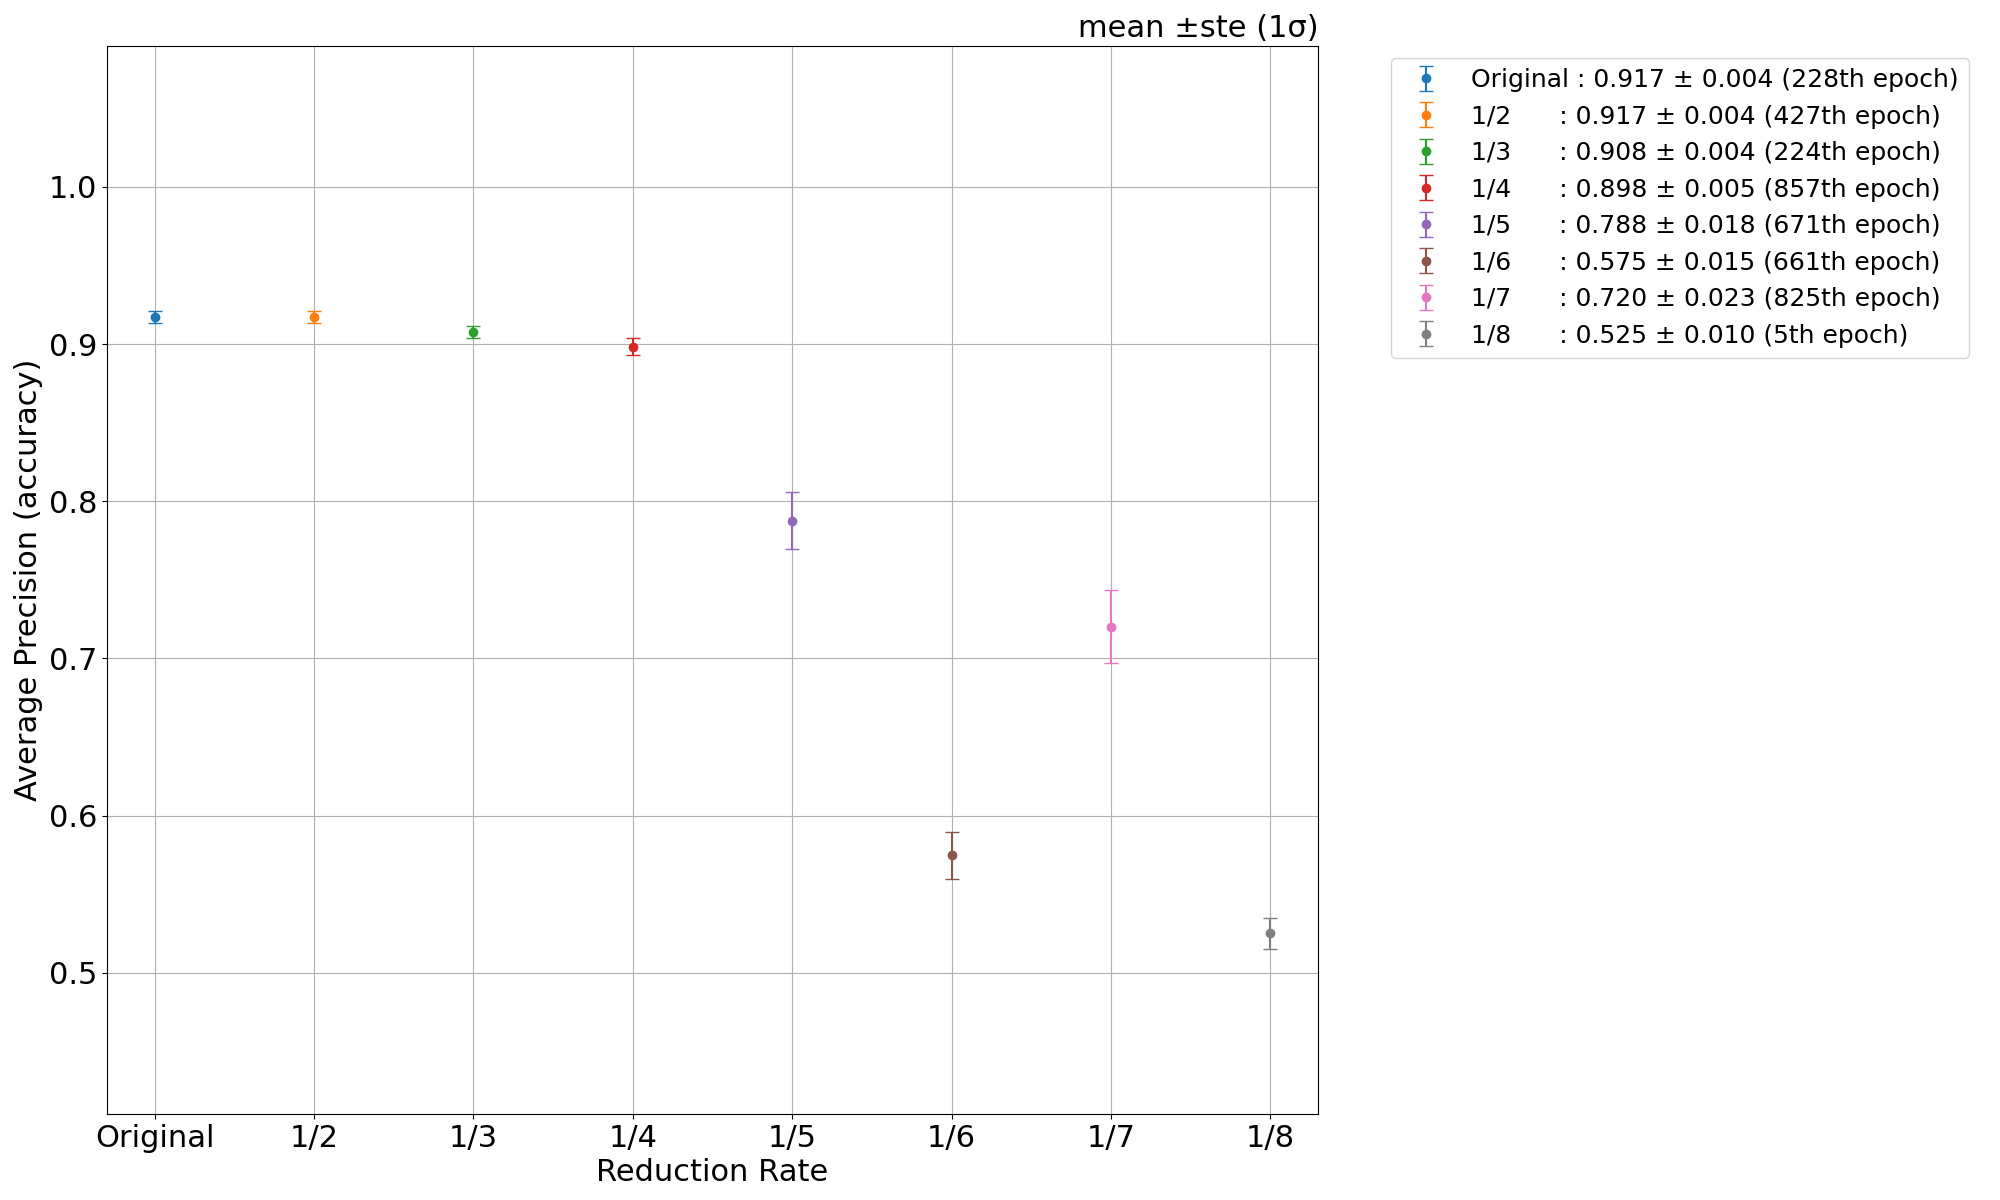
\includegraphics[width=16cm]{images/5syou/print_errorbar/linear/acc_with_errorbar_syuron5_linear_900epoch_30run_300_acc_max_ste1sigma.png}
  \caption{バイリニア補間によって内挿された,縮小データに対するモデルの予測結果(1ste)}
  \label{fig:linear_300_1ste}
\end{figure}
 
\begin{figure}[H]
  \centering
  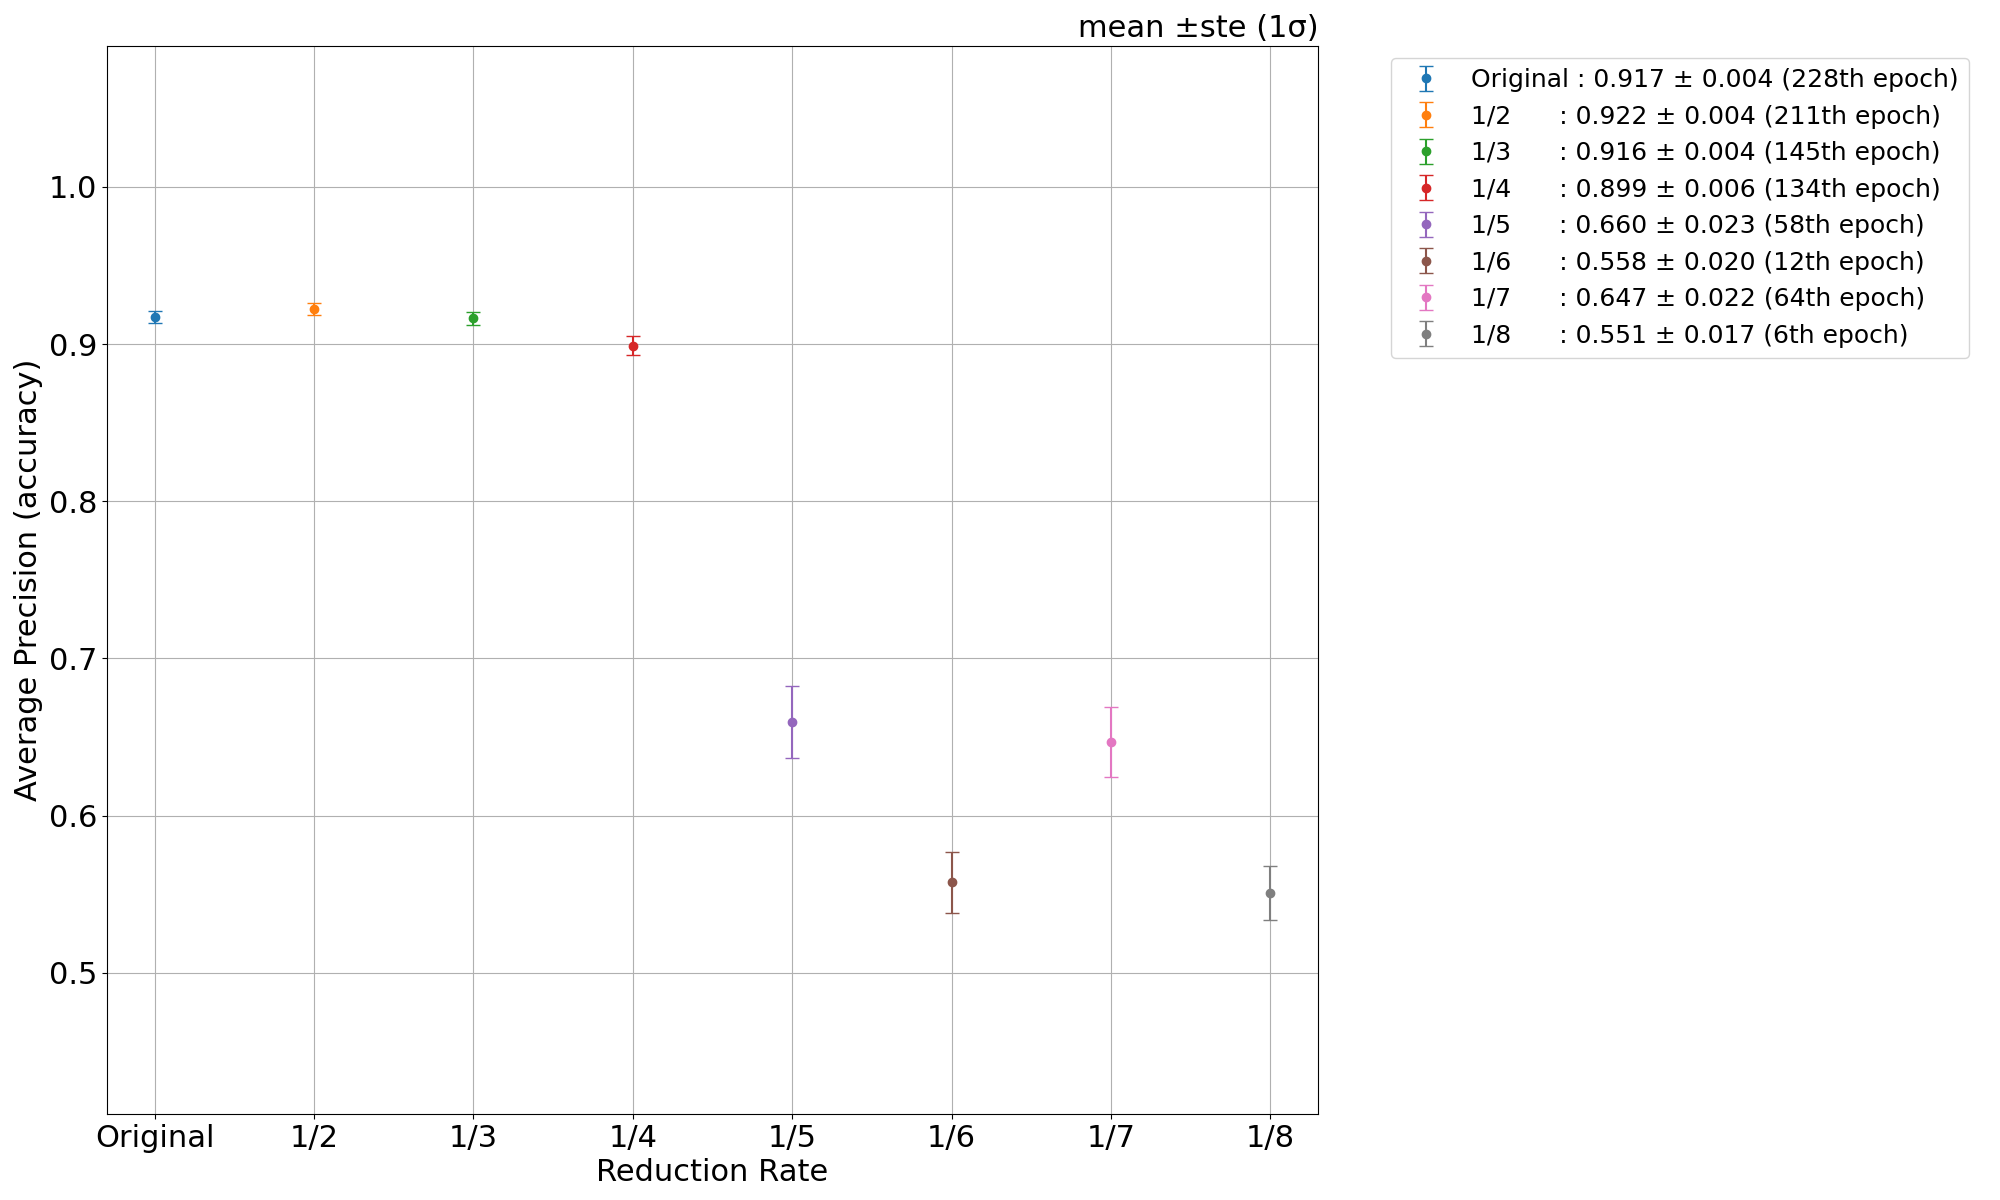
\includegraphics[width=16cm]{images/5syou/print_errorbar/cubic/acc_with_errorbar_syuron5_cubic_900epoch_30run_300_acc_max_ste1sigma.png}
  \caption{バイキュービック補間によって内挿された,縮小データに対するモデルの予測結果(1ste)}
  \label{fig:cubic_300_1ste}
\end{figure}



\newpage
\section{分類精度の使用画像枚数依存性}
本研究で掲げている将来展望として,予測精度を高く保ったまま,学習データの枚数をなるべく少なくする方が好ましい.理由としては,天体画像データセットおよびそれをもとにした形態分類カタログの完成には膨大な時間がかかるからである.

今度登場するであろう高解像度データセットだが,完成には時間がかかる.そのため,完成を待たずある程度の高解像度天体データが撮影された時点で,それらを用い高精度の分類モデルを学習し,既存の低解像度データセットに対し形態分類の予測を適用することが将来展望の構想である.そのため,形態分類の精度を高く保ったまま,どのくらいの使用天体数の少なさなら使えるかを検証することは,将来展望を議論するのに有用である.

これを検証するため,分類精度の使用画像枚数依存性について調べる.具体的には,銀河種ごとの使用天体数をそれぞれ500, 800, 1000天体とし,モデルの学習・テストを行う.5.2節で行っていた300天体の結果も合わせて,使用天体数300, 500, 800, 1000天体で行った実験におけるモデルの予測結果を,テストデータに対する予測のaccuracyをもって比較し,以下を検証する.
\begin{quote}
 \begin{itemize}
  \item テストデータに対する予測のaccuracyの,平均値・誤差(1標準偏差)の増減はあるのか,増減幅はどのくらいか
  \item ''Original''の結果(学習データとテストデータの解像度が揃っている状況での予測結果)と同程度の高精度分類を達成するテストデータの縮小倍率に,変化があるのか
 \end{itemize}
\end{quote}

\subsection{実験条件}
モデルの学習・テストには,GZによる形態分類が行われた15,000天体(図\ref{fig:z_15000}参照)を母集団とし,銀河種類ごとにそれぞれ500,800および1000天体を使用した.銀河種類ごとのデータインバランスが起こらないようにするため,渦巻銀河と楕円銀河の比率は等しくなるように選定をした.選定を行う際,赤方偏移$z$について,$0 < z < 0.2$という条件を設定し,あてはまらない天体は除外を行う.これは,地球との距離が遠すぎる天体については上手く特徴抽出が行えず学習の妨げになる可能性があるからである.

使用天体を選定した後,学習データとテストデータの比率が7:3となるように天体群を分けた.このうち,学習データにはSDSSの切り出し画像,テストデータにはSDSSの切り出し画像を縮小した画像をそれぞれ用いた.また,学習データとテストデータ内において,銀河種のデータインバランスが起こらないようにするため,渦巻銀河と楕円銀河の比率が等しくなるようにした.

モデルの評価を行う際,モデルの学習およびテストを30回行い,accuracyの平均値,標準偏差および標準誤差を導出した.
なお,30回の学習およびテストの際,学習実行毎に使用される天体は毎回シャッフルされる.

モデルの学習期間は900epochとした.これは,すべての縮小データの縮小倍率にて,モデルが学習しきる期間,すなわちテストデータに対するaccuracyが上がりきるepoch数が900epochであったからである.

\subsection{実験結果}
\subsubsection{縮小データに対する予測結果}
銀河切り出し画像を1/2倍から1/8倍に縮小した縮小データに対する,形態分類モデルの予測結果の図を図\ref{fig:nearest_num_of_gal_comparison_1std}から図\ref{fig:cubic_num_of_gal_comparison_1std}に示す.

\begin{quote}
 \begin{itemize}
  \item 横軸が,テストデータである縮小データの縮小倍率であり,縦軸がテストデータに対する予測のaccuracyとなっている.
  \begin{quote}
   \begin{itemize}
    \item テストデータに対する予測のaccuracyについて,30回実行における平均値と標準偏差(2std)をエラーバー形式で示している.
    \item なお,一番左に位置しているOriginalとなっている箇所は,テストデータに縮小データでなく,学習データと同じ大きさの銀河切り出し画像を使用してテストを行った結果である.すなわち,Originalが学習データとテストデータの解像度が揃っている状況での予測結果に対し,1/2から1/8が学習データとテストデータとの間に解像度差がある状況での予測結果を示している.
   \end{itemize}
  \end{quote}
  \item accuracyを採るepoch数は,モデルが十分に学習しきるepoch数とした.すなわち,テストデータに対するaccuracyが最大値となるepoch数とした.
 \end{itemize}
\end{quote}

\begin{figure}[H]
  \centering
  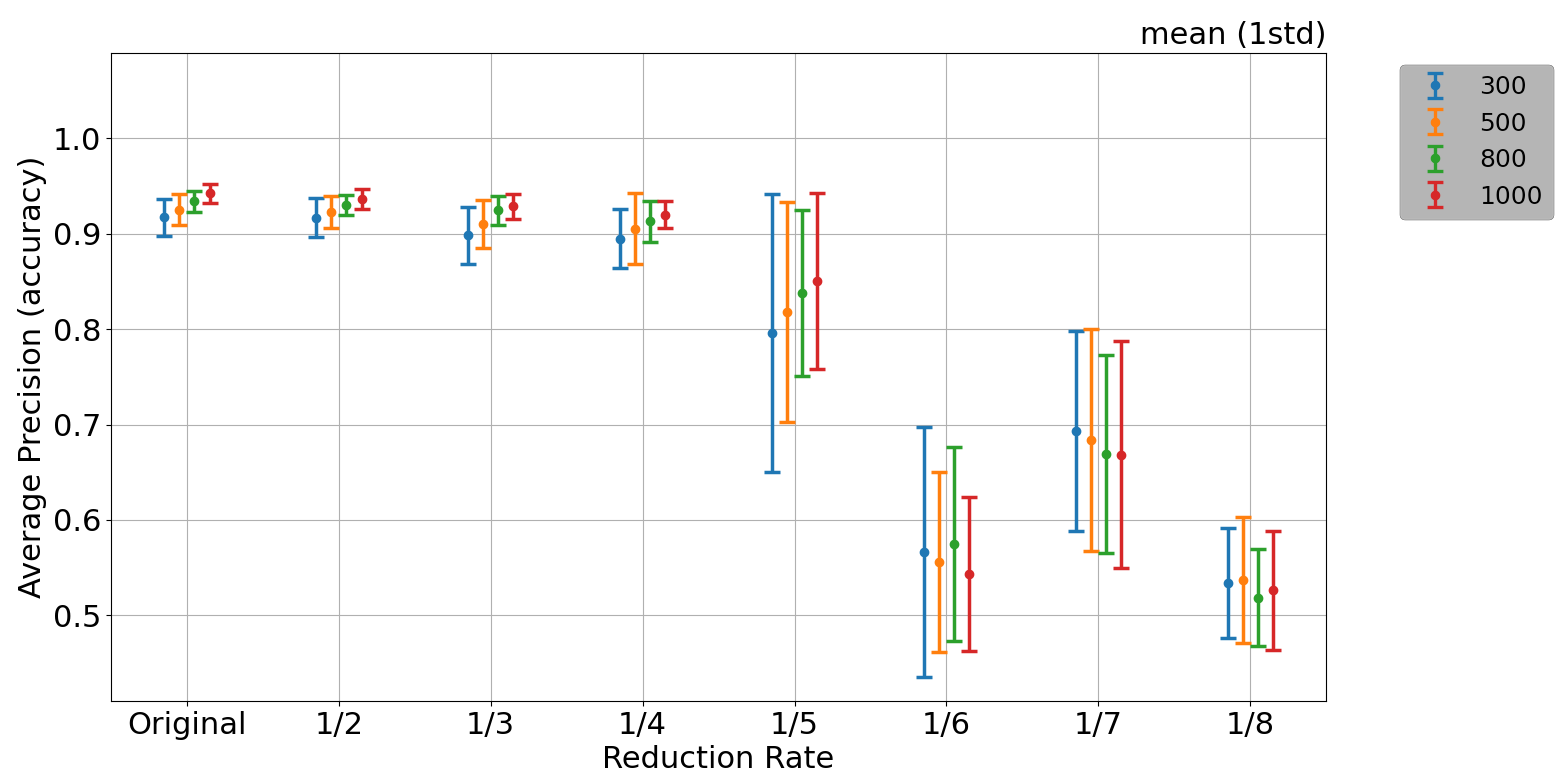
\includegraphics[width=1.0\hsize, keepaspectratio]{images/5syou/print_errorbar/nearest/acc_with_errorbar_syuron5_nearest_900epoch_30run_num_of_gal_comparison_acc_max_std1sigma.png}
  \caption{最近傍補間によって内挿された,縮小データに対するモデルの予測結果(1std)}
  \label{fig:nearest_num_of_gal_comparison_1std}
\end{figure}

\begin{figure}[H]
  \centering
  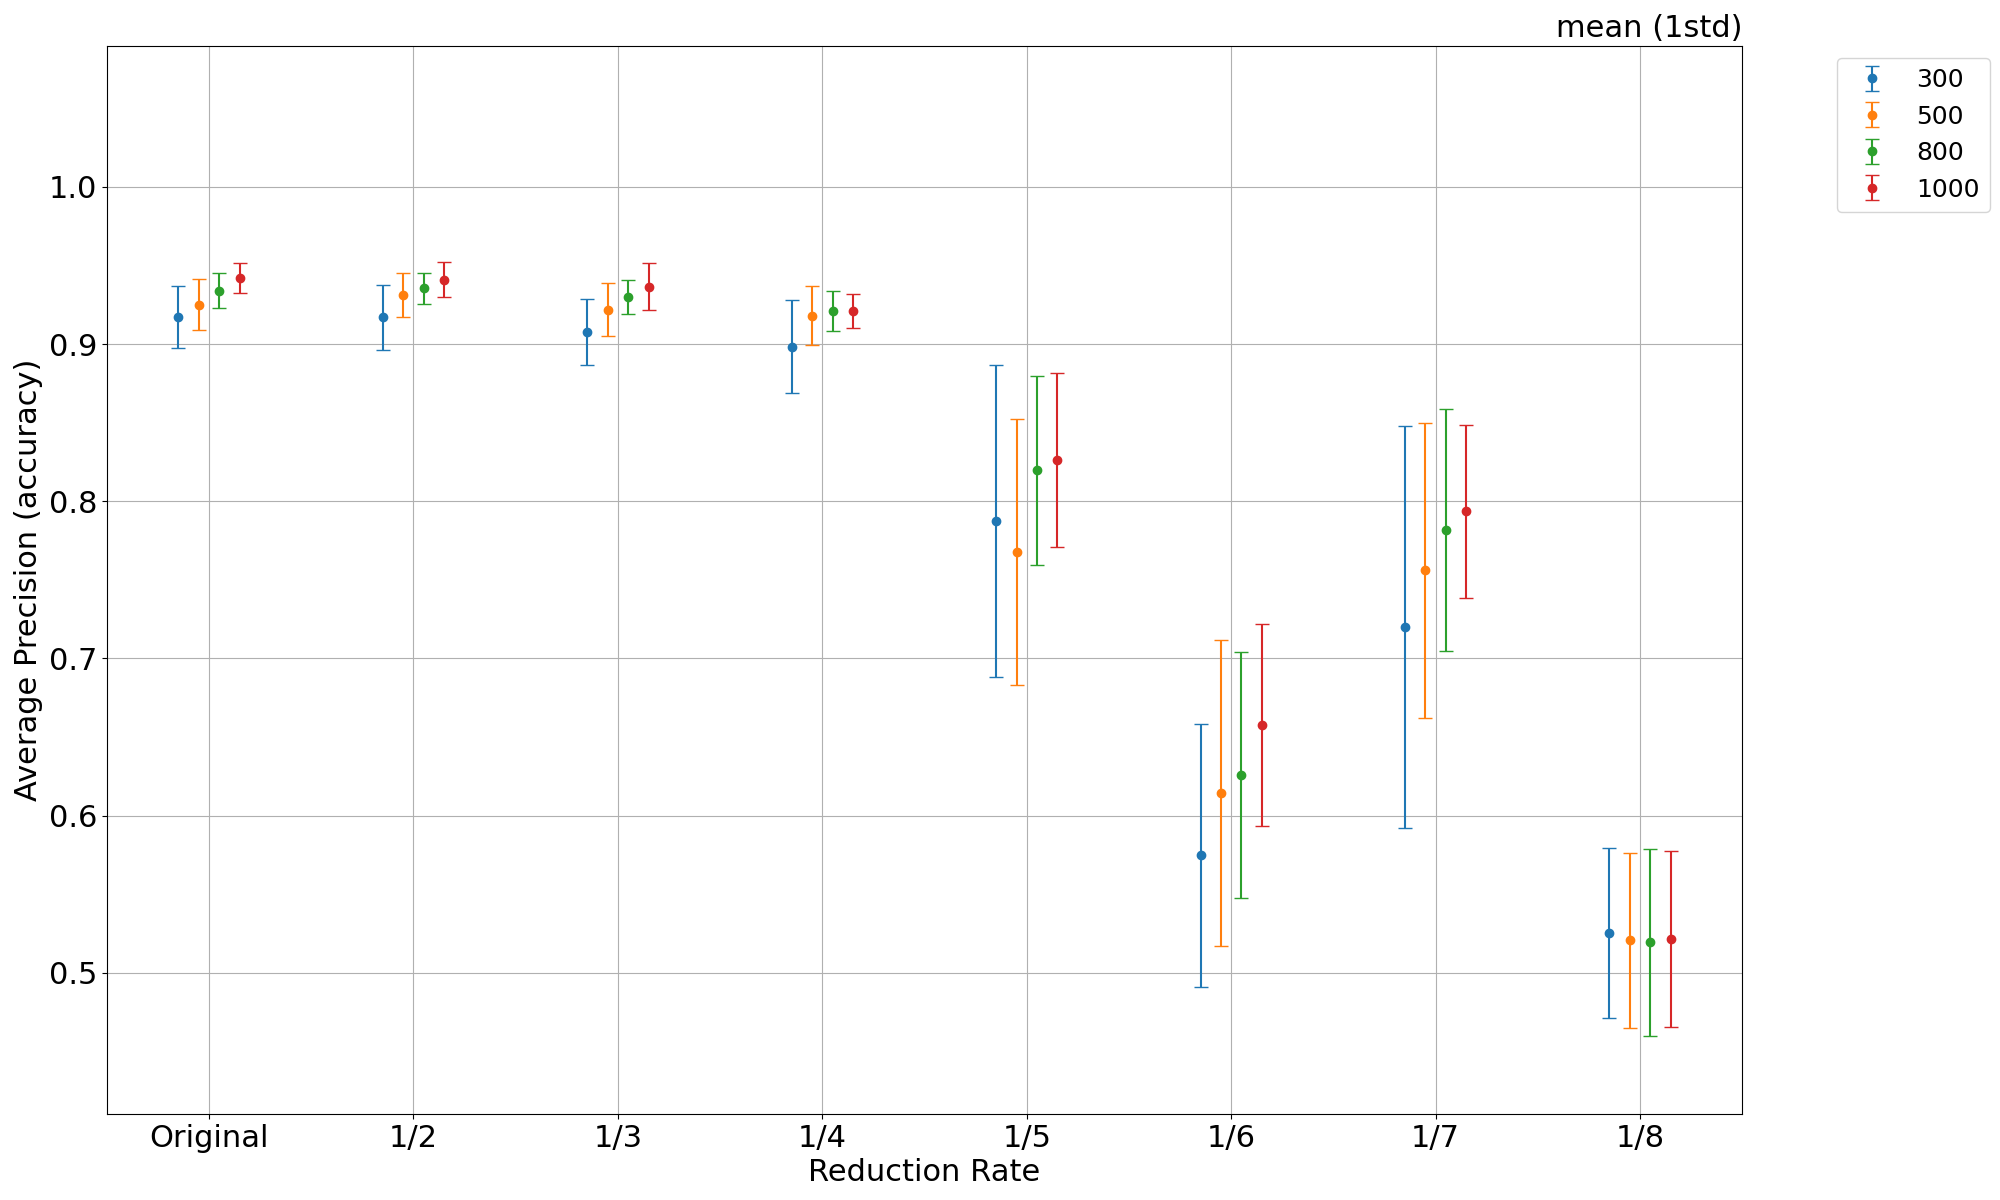
\includegraphics[width=1.0\hsize, keepaspectratio]{images/5syou/print_errorbar/linear/acc_with_errorbar_syuron5_linear_900epoch_30run_num_of_gal_comparison_acc_max_std1sigma.png}
  \caption{バイリニア補間によって内挿された,縮小データに対するモデルの予測結果(1std)}
  \label{fig:linear_num_of_gal_comparison_1std}
\end{figure}

\begin{figure}[H]
  \centering
  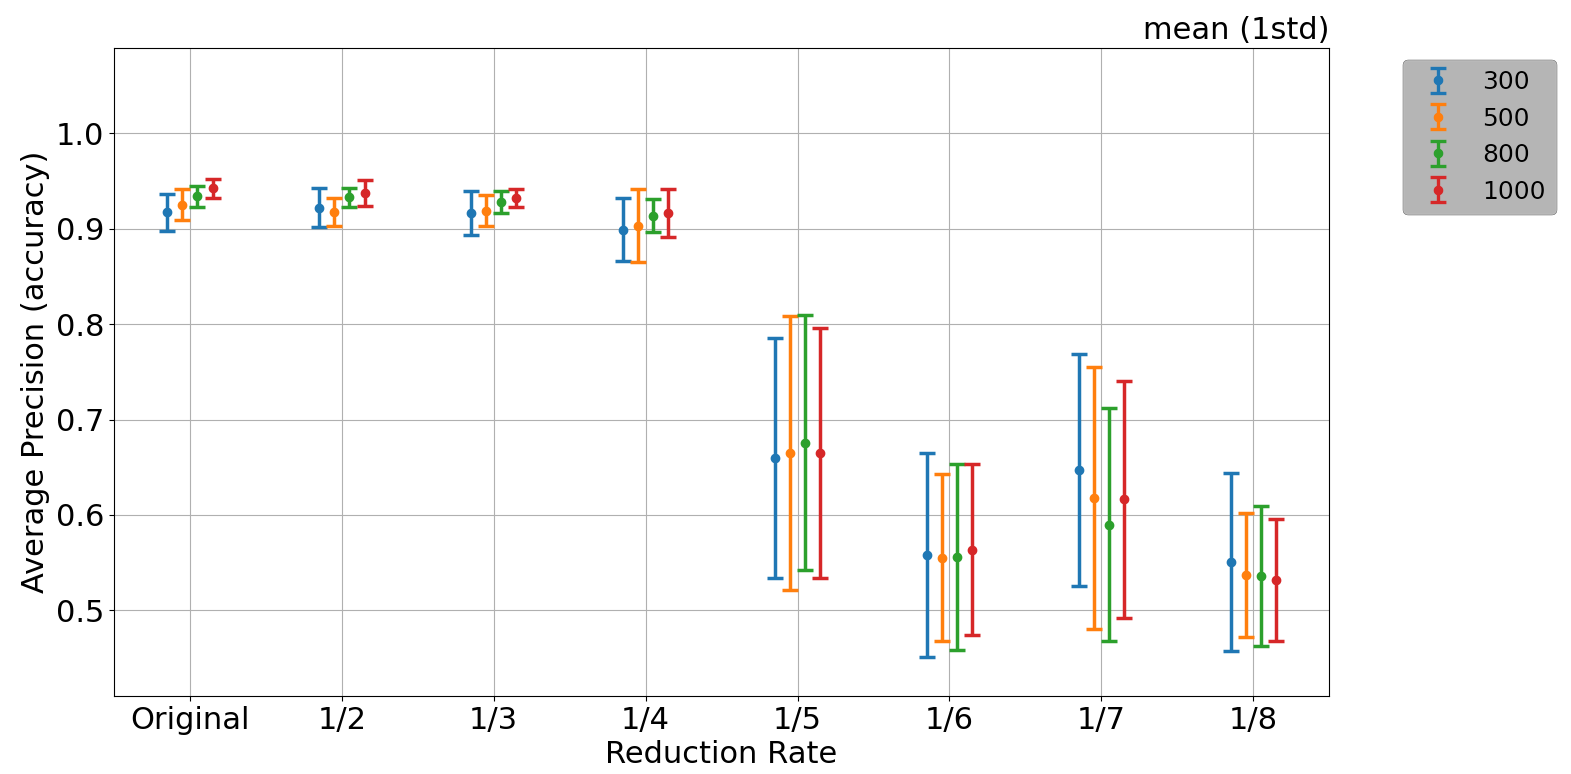
\includegraphics[width=1.0\hsize, keepaspectratio]{images/5syou/print_errorbar/cubic/acc_with_errorbar_syuron5_cubic_900epoch_30run_num_of_gal_comparison_acc_max_std1sigma.png}
  \caption{バイキュービック補間によって内挿された,縮小データに対するモデルの予測結果(1std)}
  \label{fig:cubic_num_of_gal_comparison_1std}
\end{figure}

\subsubsection{結果}
\subsubsection{使用天体数増加によるaccuracyの変化}
使用天体数を増やすことで補間方法によらず,縮小倍率が1/2倍から1/4倍の縮小画像データに対する予測のaccuracyの平均値が上昇し,また標準偏差の値も小さくなった.特に使用枚数が300枚と1000枚の結果を比較すると,標準偏差の値がおよそ半減していることが図\ref{fig:nearest_num_of_gal_comparison_1std}から図\ref{fig:cubic_num_of_gal_comparison_1std}より読み取れる.

また縮小倍率が1/5倍から1/8倍に対する予測のaccuracyについては,内挿方法によりaccuracyの挙動に差が出た.これについては\textbf{内挿方法間での比較}にて詳述する.


\subsubsection{内挿方法間での比較}
内挿方法の間で,銀河種ごとの天体使用数を増加させた際に見受けられる,テストデータに対するaccuracyの細かい挙動を比較する.なお,縮小倍率1/2倍から1/4倍のデータに対する予測結果は前段落である\textbf{使用天体数増加によるaccuracyの変化}で述べたので,ここからは縮小倍率が1/5倍以上のデータに対する結果を比較する.

最近傍補間によってテストデータの内挿を行った場合,銀河種ごとの天体使用数を増加させることで,縮小倍率1/5倍のデータに対する予測のaccuracyの平均値上昇,および標準偏差の減少が見受けられる.しかしながら,標準偏差の減少量は1/2倍から1/4倍の縮小倍率データに対する予測と比べるとそれほど大きくないことが分かる.

バイリニア補間によってテストデータの内挿を行った場合,銀河種ごとの天体使用数を1000天体まで増やしても,1/5倍から1/8倍の縮小倍率データに対する予測のaccuracyが0.9を超えず,高精度分類を行えなかった.しかしながら,銀河種ごとの天体使用数を増加させることで,縮小倍率が1/5倍から1/7倍のテストデータに対する予測のaccuracyの精度改善が見込めた.
\\なお1/8倍の縮小倍率に対する形態分類は,銀河種ごとの天体使用数および内挿方法を問わずaccuracy0.5付近を記録した.このため,学習データとテストデータとの間の解像度差が1/8倍である場合,深層学習モデルによる形態予測が行えないのではないかと思われる.

バイキュービック補間によってテストデータの内挿を行った場合,銀河種ごとの天体使用数を1000天体まで増やしても,1/5倍から1/8倍の縮小倍率データに対する予測のaccuracyが0.9を超えず,またaccuracyの平均値および標準偏差に改善が見られなかった.

\subsubsection{使用可能なデータセット間の解像度差について}
図\ref{fig:nearest_num_of_gal_comparison_1std}から図\ref{fig:cubic_num_of_gal_comparison_1std}より,内挿方法を問わず,銀河種ごとの天体使用数が何天体であっても,縮小倍率が1/4倍までの縮小データに対する予測のaccuracyが,Originalの結果(学習データとテストデータの解像度が揃っている状況での予測結果)と同程度かつaccuracyが0.9付近を記録することが読み取れる.このことから,内挿方法・銀河種ごとの使用天体数によらず,学習データとテストデータの解像度差が1/4までならば使用可能であることが分かった.
\\また\textbf{内挿方法間での比較}にて,縮小倍率が1/4倍までの縮小データに対する予測では,銀河種ごとの天体使用数を増加させることで内挿方法によらず予測精度が向上することが分かった.このことから,学習データとテストデータの解像度差が1/2倍から1/4倍ほどである2値銀河形態分類は,モデルの学習の上振れを期待せずとも,高精度の形態予測を期待できる分類問題であると思われる.

次に,学習データとテストデータの解像度差が1/5倍より大きい場合について述べる.最近傍補間によってテストデータを内挿する場合,解像度差が1/5倍のとき,銀河種ごとの天体使用数を増やすことで誤差区間が減少する.しかし,最も多い天体数である使用天体数1000天体においても,1標準偏差区間の上位25\%しかaccuracyが0.9を超えず,このことから,モデルの学習が上振れることを期待する必要があるため使用不可な解像度差であると判断した.
\\また,図\ref{fig:linear_num_of_gal_comparison_1std},図\ref{fig:cubic_num_of_gal_comparison_1std}より,バイリニア補間,およびバイキュービック補間においては,Originalの結果と同程度かつaccuracyが0.9付近を記録しないことが読み取れる.

したがって,学習データとの解像度差が1/5倍より大きいテストデータは使用不可であることがわかった.
\section{5章全体の議論・結論}
\subsubsection{どの補間フィルタを用いるべきか}
第5章では学習データに高解像度,テストデータに低解像度の画像データを使用していた.深層学習モデルに入力する画像データは全て同じサイズである必要があるため,今回の実験ではテストデータである低解像度画像を拡大を行った.\\ここで,今回の画像拡大に用いた3手法(最近傍補間・バイリニア補間・バイキュービック補間)のうち,どれを使うべきかを考察する.

まず,第5章にて''使用可能''と定義した,学習データとテストデータとの間の解像度差が1/2倍から1/4倍の状況でモデルの学習・それによる予測を行う場合について考察する.図\ref{fig:nearest_num_of_gal_comparison_1std}から図\ref{fig:cubic_num_of_gal_comparison_1std}より,どの天体使用数においても,3つの拡大手法でのaccuracyは同程度の挙動,なおかつ0.9付近のスコアを記録している.このことから,学習データとテストデータとの間の解像度差が1/2倍から1/4倍の状況でモデルの学習・それによる予測を行う場合,これら3手法のどれを使用しても高精度の予測が行えると考えられる.
\\ただし図\ref{fig:cubic_num_of_gal_comparison_1std}より,バイキュービック補間は使用天体数を増やした際のaccuracy平均値向上・誤差低下の恩恵を受けづらいことが読み取れる.

次に,第5章にて''使用不可''と定義した,学習データとテストデータとの間の解像度差が1/5倍から1/8倍の状況でモデルの学習・それによる予測を行う場合について考察する.この場合,5.3.2の結果における\textbf{内挿方法間での比較}より,使用天体数を増加させた際のaccuracy平均値向上・誤差低下が最も見込めるバイリニア補間が適していると思われる.

最後に,3つの拡大手法の処理にかかる時間を考える.時間計測を行うため,SDSSから取得した銀河切り出し画像を1/8倍に縮小した縮小画像を,GZの分類ラベルにてラベル付けされた渦巻銀河50天体・楕円銀河50天体について拡大処理を実行した.拡大処理は各手法にてそれぞれ10000回ずつを7周実行し,拡大にかかった時間の平均値および1標準偏差を導出した.
\\表\ref{tb:calc_cost_by_interpolation}に3つの拡大手法の処理にかかる時間を示す.表より,最近傍補間が最も処理が軽く,バイリニア補間が2番目,バイキュービック補間が3番目に処理に時間がかかることが読み取れる.

上で述べた3つを総合的に考慮すると,モデルの学習・テストにおける処理を最も軽くしたい場合は最近傍補間が望ましいと考えられる.
\\また処理が少し重くてもよく,使用天体数を多くした際のaccuracyに対する恩恵を受けたい場合はバイリニア補間による内挿がよいと思われる.
\\バイキュービック補間は,使用天体数を増加させた際のaccuracyに対する恩恵を最も受けづらく,また拡大処理における処理の重さを考えると,3手法の中では使用する意味が最も薄いと考えられる.

\begin{table}[htbp]
  \centering
	\caption{各補間フィルタによる拡大の計算コスト(平均値(1標準偏差))}
  \begin{tabular}{|c|c|}
		\hline
    最近傍補間 & $247\mu s \pm 2.25\mu s$ \\ \hline
    バイリニア補間 & $378\mu s \pm 5.37\mu s$ \\ \hline
    バイキュービック補間 & $1.48ms \pm 7.74\mu s$ \\ \hline
  \end{tabular}
  \label{tb:calc_cost_by_interpolation}
\end{table}

\subsubsection{学習データとテストデータとの間の解像度差が1/6および1/7の際の,テストデータに対する予測accuracyの挙動}
第5章にて使用天体数・内挿方法を問わず共通の傾向であった,「縮小倍率が1/7倍の縮小データに対する予測精度が,縮小倍率1/6倍の予測精度より高い」事に対し,考察を行う.

一般的に,テストデータの解像度が低ければ低いほど,分類モデルによる予測精度は低くなると考えられる.図\ref{fig:nearest_num_of_gal_comparison_1std}から図\ref{fig:cubic_num_of_gal_comparison_1std}においても,縮小倍率が1/2倍から1/6倍においては上記の傾向が見受けられる.しかしながら,1/7倍の縮小倍率に対する予測精度は,1/2倍から1/6倍にて見受けられた傾向から逸脱している.この傾向に対し,考察を行う.

1/6倍, 1/7倍の縮小画像に対する画像拡大例を図\ref{fig:1_6and1_7}に示す.図\ref{fig:1_6and1_7}より,拡大手法によって生成される画像が,見かけではかなり異なることが分かる.しかし,図\ref{fig:nearest_num_of_gal_comparison_1std},図\ref{fig:linear_num_of_gal_comparison_1std}を比較すると,拡大手法によって縮小倍率1/6倍と縮小倍率1/7倍のaccuracyの挙動に大きな差はないことが分かる.ここで,1/6倍,1/7倍の縮小画像(図\ref{fig:1_6and1_7}の左下)を見ると,画像内の最も明るいピクセルが存在する場所に差があることが分かる.1/6倍の縮小画像では中央より右下,1/7倍の縮小画像では中央が一番明るいピクセルであることが読み取れる.このことから,平均画素法による縮小の際,何らかの形で銀河の形態的特徴が損失している可能性がある.そしてこの形態的特徴損失により,学習データとテストデータとの間の解像度差が1/6および1/7の際の,テストデータに対する予測accuracyの挙動に影響を及ぼしていると思われる.

\begin{figure}[htbp]
 \centering
 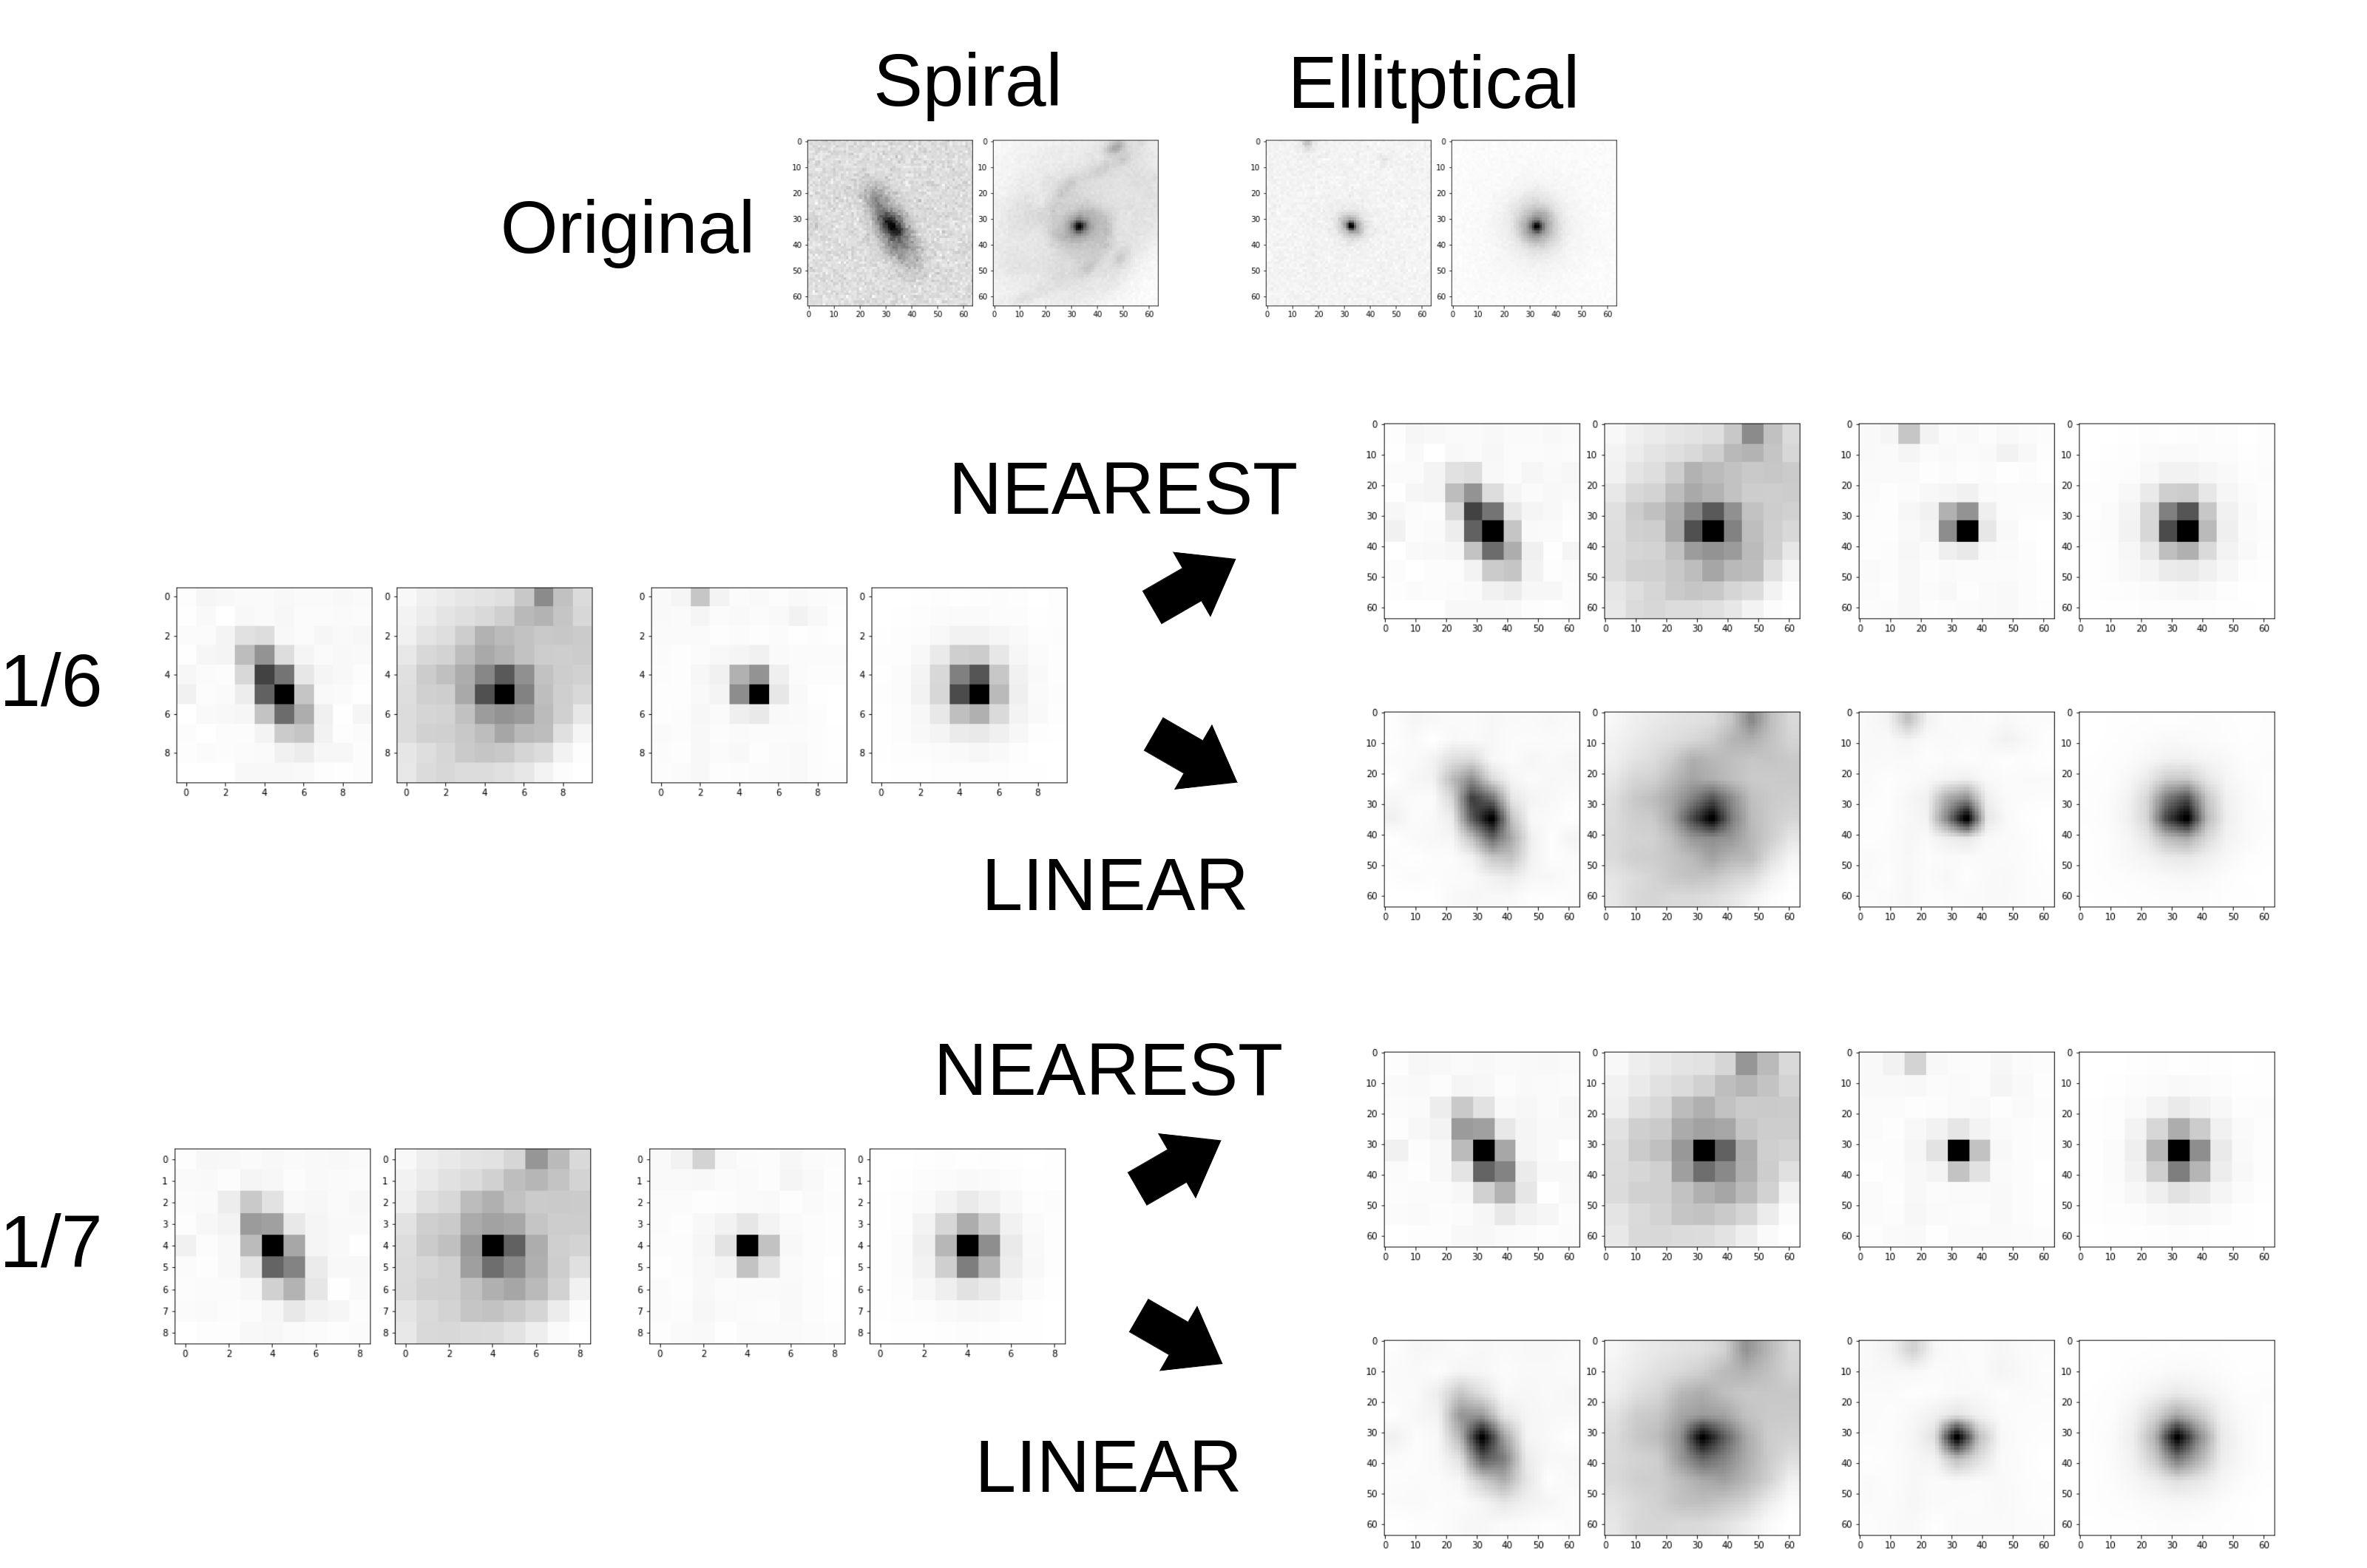
\includegraphics[width=1.0\hsize, keepaspectratio]{images/5syou/syuron_5syou_kakudai/ver1/5syou_giron_1_6and1_7.png}
 \caption{1/6倍, 1/7倍の縮小画像に対する画像拡大例(最近傍補間・バイリニア補間)}
 \label{fig:1_6and1_7}
\end{figure}


\subsubsection{使用枚数が何枚までならば高精度を保てるか}
最後に,モデルの学習・テストに用いる銀河種ごとの天体使用数について,形態分類の精度を高く保ったまま,どのくらいの使用天体数の少なさなら''使用可能''かについて議論を行う.なお,第5章全体を通して''使用可能''と定義している学習データとテストデータとの間の解像度差が1/2倍から1/4倍の状況に限定して,使用天体数の議論を行う.

図\ref{fig:nearest_num_of_gal_comparison_1std}から図\ref{fig:nearest_num_of_gal_comparison_1std}より,使用する天体数は何天体でもよいと思われる.これは,内挿方法を問わず,''Original''と同程度の予測精度,すなわちaccuracyが0.9程度をスコアするからである.ここでテストデータに対する予測のaccuracyを0.9以上にしたい場合だが,図\ref{fig:nearest_num_of_gal_comparison_1std}から図\ref{fig:nearest_num_of_gal_comparison_1std}より,これは銀河種ごとの天体使用数を800天体以上にすることが望ましいと考えられる.

この章では,「学習データとテストデータとの間の解像度差がある状況において,分類モデルの学習が行えるか」の検証を行うため,2つの実験を行った.

学習データとテストデータとの間の解像度差が1/4までならば,内挿方法によらず使用可能,すなわち学習データとテストデータの解像度が揃っている状況での予測結果である”Original” と同程度の高精度な分類,すなわちaccuracy が0.9 付近を記録する結果となった.

銀河種ごとの使用天体数を増加させた際,テストデータに対する予測のaccuracyの挙動は内挿方法によって差が生じた.最近傍補間による内挿では,1/2倍から1/5倍までの縮小倍率画像に対し精度改善が見込めた.バイリニア補間に関しては,1/2倍から1/7倍までの縮小倍率画像に対し精度改善が見込めた.バイキュービック補間は1/2倍から1/4倍までの縮小倍率ならば精度改善が見込めたが,他2手法よりもその恩恵は小さく,更に1/5倍より大きい縮小倍率画像に対する予測精度は改善が見込めなかった.

内挿方法によってテストデータに対する予測精度が異なる挙動を見せることから,モデルへの内挿方法を模索することで,更なる精度改善,および本研究では使用不可と判断した学習データとテストデータとの間の解像度差においても,高精度分類が行える可能性がある.

\newpage
\chapter{議論}
\section{本研究のまとめ}
本研究の将来展望は,高空間分解能観測装置データを用いてモデル学習を行うことで,既存の低空間分解能データセットに対し更なる高精度形態分類を提供するというものである.この将来展望が実現できる可能性を検証するため,本研究では第4章,第5章にて将来展望の前段階となる実験群を行った.その結果,深層学習による銀河形態分類の主に渦巻銀河・楕円銀河に分類する2値分類問題において,学習データとテストデータとの間に1/4倍の画像解像度差が生じていても,テストデータに対しaccuracyが0.9付近となる高精度分類が提供できることが分かった.このことから,将来展望である「異なる観測装置データの組み合わせを行い,深層学習による銀河形態分類」を実現できる可能性が示された.

一方で,SDSS DR7とGZ1を組み合わせた深層学習による形態分類の更なる精度向上など,多くの将来課題が残されている.6.2節ではそれらについて言及を行う.

\section{将来課題}
\subsubsection{深層学習モデルの分類精度向上}
\textbf{この節で見せたい実験結果(SDSSを1/8倍に縮小した画像にてモデル学習,それをSDSS1/8倍縮小画像にてテスト)について,この実験結果を見せたい場合,モデル学習・テストを30回実行した結果ではなく1回だけ実行した結果を見せることになる.この1回実行の結果をもとにここの議論を行うか,ここだけ30回実行した結果を見せるか,火曜日の議論時に相談させていただければと思います.}

本研究にて扱ったSDSSとGZを用いた深層学習分類モデルについて,これは更なる分類精度の向上が望めると考えられる.例として,当論文第4章では渦巻銀河および楕円銀河と分類する2値分類問題を約93\%のAccuracyで分類した.
ここで,Dieleman et al.(2015)\cite{Dieleman2015}ではSDSSの天体画像とGalaxy Zoo 2の銀河形態分類ラベルを学習データに用いて深層学習銀河形態分類モデルを学習し,GZ2の形態分類を約99\%のAccuracyで再現した.Dieleman et al.と本研究は用いる銀河画像データは同じSDSSであるが,再現する形態分類は本研究が2値分類であるのに対しDieleman et al.は37値分類であり,Dieleman et al.の方がより難しい分類問題を解いているといえる.
本研究はDieleman et al.より難易度の低い分類問題を扱っているが,分類精度はそれに劣っていることから,本研究における深層学習分類モデルは,更なる分類精度向上を行う余地があると考えられる.

深層学習分類モデルの精度向上法としては,まず用いる天体画像データを単色ではなく複数色用いることが可能性の一つとして考えられる.Dieleman et al.にて,グレースケール天体画像を用いた場合とカラー天体画像を用いた場合とでは,後者の方が予測精度が大幅に向上することが報告されている.また,データ拡張などの過学習対策を行うことで分類精度を向上させられる可能性がある.本研究と同じ渦巻銀河と楕円銀河を見分ける2値分類問題を扱うCheng et al.では,過学習対策として2,103個の渦巻銀河,759個の楕円銀河をデータ拡張により約10万個まで増加させ,分類モデルの学習・テストに用いており,結果として99\%のAccuracyで分類を行っている.

\subsubsection{未知天体データセットへの予測適用方法}
\textbf{この節は,本研究を用いたい人(形態ラベル付が行われていないデータセットに対し,本研究の手法を適用したい人)向けの節でしたが,将来展望ではなく,話が纏まらないのではないかと思ったので削除しました.}

\subsubsection{GZ1の不確かを,深層学習でどう扱うか}
本研究で用いた銀河形態分類カタログであるGZには,Galaxy Zoo 1とGalaxy Zoo 2の2種類のプロジェクトが存在する.両者の大きな差異として,銀河形態分類の詳細性と調査が行われた天体数が候補としてあげられる.Galaxy Zoo 1では銀河を6つのカテゴリに,Galaxy Zoo 2では37つのカテゴリへと分類し,このことから銀河形態分類の詳細性はGalaxy Zoo 2の方が高い.しかし,Galaxy Zoo 1で形態分類が行われた天体は約90万天体,Galaxy Zoo 2においては約30万天体であり,よって調査が行われた天体数はGalaxy Zoo 1の方が多い.これら2つを考慮した際,Galaxy Zoo 1において形態分類の正確性を向上すれば,より多数の天体に対し形態分類ラベルが適用できる為有用であると考えられる.


\section{将来展望}
本研究にて異なる観測装置データの組み合わせによる深層学習形態分類の可能性が示された.そこで,ここからは実際に異なる観測装置データの組み合わせを行った結果を示す.本実験では,学習データに高空間分解能観測装置から取得した天体画像,テストデータに低空間分解能観測装置から取得した天体画像を使用し,天体を渦巻銀河および楕円銀河に分類する2値分類モデルの学習およびテストを行った.そして学習を行った当該モデルの分類結果を,学習データとテストデータに同じ観測装置の天体画像データを用いた分類結果と比較した.

まず,学習データに用いた各種データについて説明を行う.
学習データに用いる高空間分解能観測装置から取得した天体画像データには,Hyper Suprime-Cam Subaru Strategic Program(HSC-SSP)\cite{Tampo2020}から取得した銀河切り出し画像を用いた.HSC-SSPとはすばる望遠鏡に装着された巨大CCDカメラであるHyper Suprime-Cam(HSC)を用いて行われている宇宙撮像サーベイである.HSC-SSPは調査領域および対応する深さをもつ3つのフィルターを使い分け,天体物理学上の様々な疑問を解決することを目的としている.また,学習データのうち低空間分解能観測装置から取得した天体画像データには,当論文の第4,5章にて用いたSDSSより取得した銀河切り出し画像を使用した.ここで,HSCの空間分解能が0.168''/pix,SDSSの空間分解能は0.369''/pixであり,これらの空間分解能の差は2.3571...倍である.この空間分解能の差は,第5章にて結論付けた''使用可能''である解像度差の範囲内である.また,HSC-SSPから取得した画像とSDSSから取得した画像において,銀河切り出し画像内の物理スケールを揃えるため,HSC-SSPの銀河切り出し画像のサイズは2つのデータセットの空間分解能差を参考に定めた.SDSSの銀河切り出し画像のサイズは64x64ピクセルであり,2つのデータセットの空間解像度差は2.3571...倍であるため,HSC-SSPの銀河切り出し画像のサイズは$(64,64) * 2.3571... \approx (150,150)$とした.

学習データのうち銀河形態ラベルについて,HSC-SSPの銀河画像に対し人間の目による分類を行った形態分類カタログが存在しなかった.そのため,GZ1による分類ラベルを流用した.具体的な使用方法として,GZによって形態分類が行われた天体と同じ天体をHSC-SSPにて検索し,HSC-SSPに存在した場合は銀河画像を取得した.

次に,その他の実験条件について述べる.モデルの学習およびテストの際に用いる天体数は1000天体とした.学習データとテストデータの比率は当論文4,5章と同じく7:3とした.また,学習データとテストデータにおける渦巻銀河と楕円銀河の比率は等しくなるようにした.分類モデルの形状は,4,5章と同じものを採用した.ここで,使用する画像データにHSC-SSPのものが含まれている場合,モデルへの入力のサイズは(150,150)とした.また,学習データとテストデータに異なる観測装置データを用いている場合は,テストデータである低解像度データを最近傍補間を用いて拡大し,データセット内のサイズを揃えた.モデルの評価は4,5章とほぼ同じ方法を採用した.具体的には,各条件におけるモデルの学習およびテストの実行回数は,第4,5章より多い実行回数である100回とした.モデルの学習およびテストを100回実行し,評価指標であるAccuracyの平均値と標準偏差を導出した.

以下に実験の結果を掲載する.テストデータに対するAccuracyの平均値と1標準偏差を導出した結果を図\ref{fig:6syou_zikkenn}に示す.図\ref{fig:6syou_zikkenn}において,横軸には3つの実験条件が示されており,左から順番に,学習データとテストデータにSDSS画像を用いた場合,学習データにHSC-SSP画像・テストデータにSDSS画像を用いた場合,学習データとテストデータにSDSS画像を用いた場合の結果である.また縦軸にはAccuracyが示されており,図中にはAccuracy平均値および1標準偏差が描画されている.なお,図\ref{fig:6syou_zikkenn}には,モデル学習およびテストを100回実行した後,テストデータに対する分類精度の平均値が最も高いepochのAccuracyを記載している.
図\ref{fig:6syou_zikkenn}より,異なる観測装置データの組み合わせによって学習されたモデルは,他2つと1標準偏差において有意な差が見受けられる.HSC-SSPとSDSSの解像度差は第5章で報告した''使用可能''の範囲内であるにもかかわらず,実際に異なる観測装置データの組み合わせで学習したモデルは学習データとテストデータに同じ観測装置データを用いたモデルの予測結果に有意差が見受けられるほど劣っていることが分かった.また,図\ref{fig:6syou_zikkenn}において,SDSSの画像データのみを使用した実験結果である左端とHSC-SSPの画像データのみを使用した実験結果である右端を比較すると,これらの結果の間に1標準偏差において有意差が見受けられないことが分かる.一般的に学習に用いる画像データの解像度は高いほど,分類精度は高くなると思われる.しかし今回の実験結果では画像の解像度による分類精度の有意差は見られない.したがって,HSC-SSPを学習データに用いた分類モデルの更なる分類性能の向上が望まれる.

SDSSの画像データのみを使用した分類モデルの分類精度とHSC-SSPの画像データのみを使用した分類モデルの分類精度に有意差が見られない理由について,これは2つの可能性が考えられる.
1つ目は,GZの形態分類が間違っていることにより,分類モデルの汎化性能が低下することである.例として,実際は渦巻銀河である天体に対しGZにて楕円銀河というラベル付けが為された状況を考える.この状況は,SDSSの空間解像度では渦巻銀河の腕がぼやけており楕円銀河に見えるものの,HSCはSDSSより高い空間分解能を有するためHSC-SSPから取得した画像では渦巻銀河に見えることが考えられる.
この場合,分類モデルがHSC-SSPの天体画像を用いて当該天体に対する学習を行った際,渦巻銀河の特徴をもつ天体を楕円銀河として学習する.このような学習が頻発した場合,学習データに対するAccuracyはepochを重ねるほどに上昇していくが,テストデータに対するAccuracyは下がってしまう.このことが,HSC-SSPの画像データのみを使用した分類モデルの分類精度が向上しない原因である可能性がある.

2つ目は,HSC-SSPの画像データを用いてモデル学習を行う場合,使用する天体数が少ないことが考えられる.深層学習モデルにおいて,全結合層のパラメータ数は入力データのサイズにより増減する.例として,入力データのサイズが大きくなると,全結合層のパラメータ数は増加する.このことは,学習データにSDSSの画像データを使用したモデルとHSC-SSPの画像データを使用したモデルでは,後者の方がパラメータ数が多いことを説明する要素である.ここで,今回行った実験において使用した天体の数は全て等しいため,学習データにSDSSの画像データを使用したモデルでは使用した天体の数が十分であったものの,学習データにHSC-SSPの画像データを使用したモデルにおいては天体数が十分でなく,モデル内のパラメータ更新回数が不十分であった可能性がある.このことが,テストデータに対するAccuracyが低いことに繋がっている可能性が考えられる.

\begin{figure}[H]
  \centering
  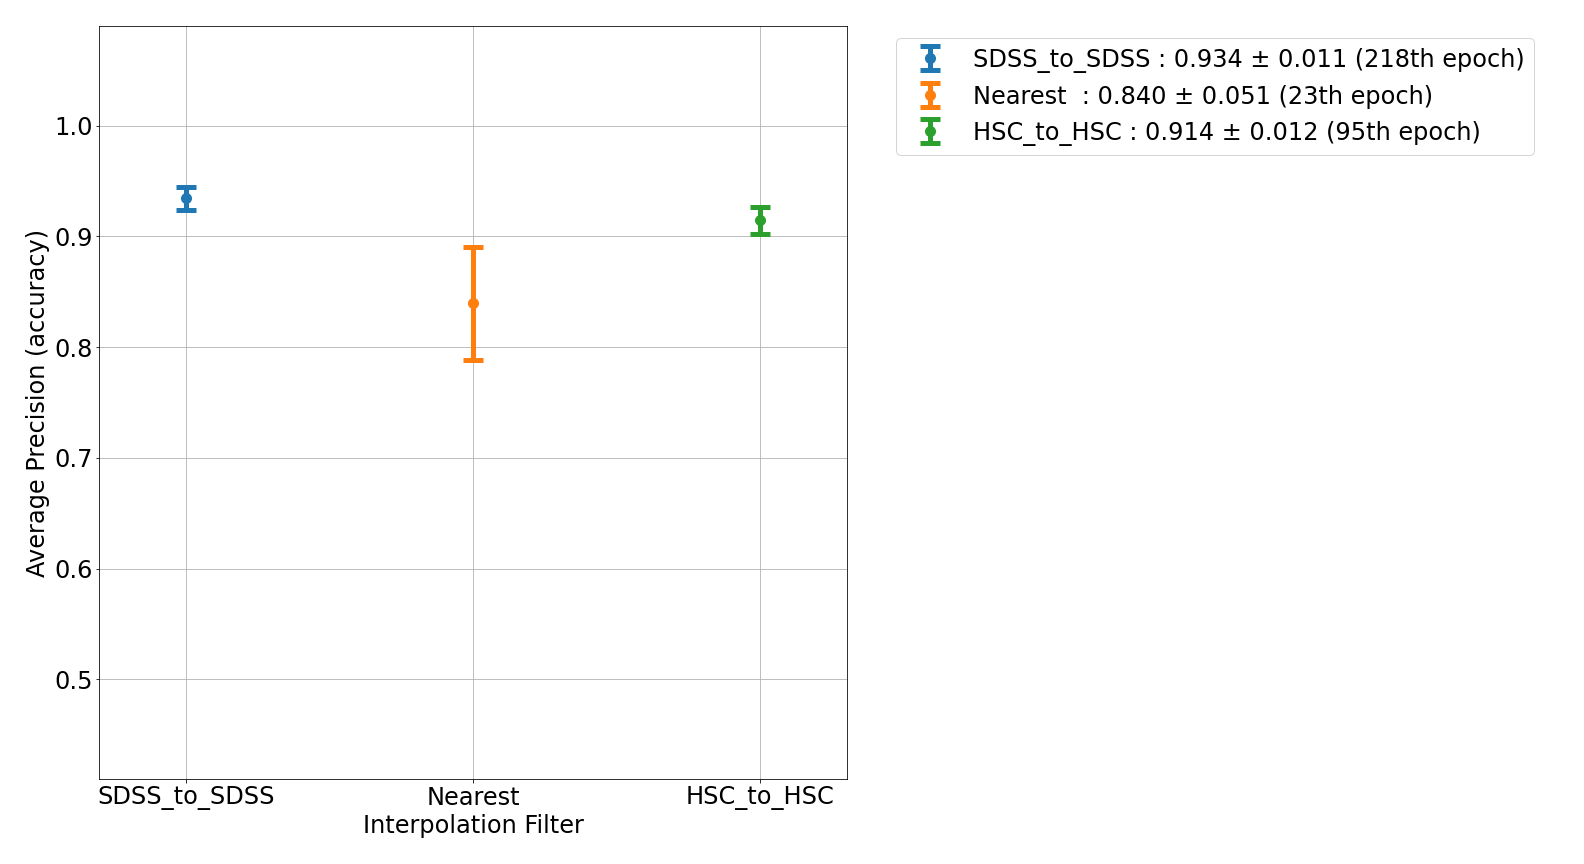
\includegraphics[width=1.0\hsize, keepaspectratio]{images/6syou/acc_with_errorbar_auto_epoch.png}
  \caption{3つの条件の分類モデルにおける,テストデータに対するAccuracy(1標準偏差)}
  \label{fig:6syou_zikkenn}
\end{figure}


\newpage
\chapter{おわりに}
本研究では,深層学習による銀河形態分類問題にて,異なる観測装置データを組み合わせて高精度な分類モデルが開発できるかを検証した.具体的には,SDSSから取得した切り出し画像とそれを縮小した縮小画像を用意した.そして異なる観測装置データの組み合わせを念頭に置き,用意した2種類のデータを組み合わせたデータセットにて分類モデルを学習させ,テストデータへの予測が成立するか,また学習データとテストデータとの間の解像度差がどれほどまでならば高精度な予測が行えるかを検証した.その結果,学習データとテストデータとの間に1/4倍の画像解像度差が生じていても,テストデータに対しaccuracy0.9程の高精度分類を行うことができた.このことから,異なる観測装置データを組み合わせて高精度な分類モデルが開発出来る可能性が示された.

今後の課題として,
\begin{inparaenum}[(1)]
 \item SDSSとGZを用いた深層学習銀河形態分類モデルの更なる精度向上
 \item 高空間解像度画像データ(HSC画像データ)を用いた深層学習モデルにおけるモデル改善
\end{inparaenum}
を目指す.
% END:本編----------------------------------------

% START:参考文献----------------------------------
%% ベタ打ちの場合
% \begin{thebibliography}{1}
% \bibitem{key1}サイト名\\ \url{http://google.com} (yyyy年mm月dd日アクセス) % ウェブサイトの場合
% \bibitem{key2}著者,書籍タイトル,出版                                      % 書籍,論文の場合
% \end{thebibliography}


%% bibtexを使用する場合
\newpage
\bibliography{Master_thesis_bib}         % .bibファイルから拡張子を外した名前 ex)ref.bib
\bibliographystyle{junsrt} % 参考文献出力スタイル
% \nocite{*}                 % 参照していない項目も出力する
% END:参考文献------------------------------------


\newpage
\chapter*{謝辞}
本研究を進めるにあたり,ご指導を頂いた新潟大学の飯田佑輔准教授,および東京理科大学の大井渚様,そしてデータセット作成や宇宙関連知識取得に際し多大な助力をいただいた同研究室の津田様に,厚く感謝申し上げます.\\
また,日常の議論を通じて多くの知識や示唆を頂いた飯田佑輔研究室の皆様に感謝いたします.

SDSSおよびSDSS-IIの資金はアルフレッド・P・スローン財団から提供され,また参加機関は米国科学財団,米国エネルギー省,米国航空宇宙局,日本の文部科学省,マックスプランク協会,英国高等教育基金協会です.SDSSのWebサイトは,http://www.sdss.org/ です. 

SDSSは参加機関のための天体物理学研究コンソーシアムによって運営されています.参加機関は,アメリカ自然史博物館,ポツダム天体物理学研究所,バーゼル大学,ケンブリッジ大学,ケース・ウェスタン・リザーブ大学,シカゴ大学,ドレクセル大学,フェルミラボ社,高等研究所,日本参加グループ,ジョンズ・ホプキンス大学,原子核宇宙物理学合同研究所,カブリ粒子宇宙物理学研究所,韓国科学者グループ,中国科学者グループ,中国科学者グループ,韓国科学者グループ 韓国科学者グループ,中国科学院(LAMOST),ロスアラモス国立研究所,マックスプランク天文学研究所,マックスプランク天体物理学研究所,ニューメキシコ州立大学,オハイオ州立大学,ピッツバーグ大学,ポーツマス大学,プリンストン大学,米国海軍天文台,ワシントン大学です.

\end{document}
%------------------------------------------------
